\section{Standard Model Background Estimation} \label{sec::BGestimation}
Due to the enormously large cross-section of SM processes with respect to the signal,
it is a fate for new physics searches to keep exploring the phase space with tight event selections.
The consequence is the highly untypical kinematics for the remained SM backgrounds, and the modeling is usually challenging since the standard MC simulation is not necessarily reliable as we will see in Sec. \ref{sec::BGestimation::dataMC}. \\

This is why (semi-)data-driven approach is remarkably motivated in search analyses. 
The most commonly done practice over the past analyses is to apply an in-situ correction to MC using the data events around signal region (``control region''). The prediction in signal regions is the given by the corrected MC, assuming the modeling on the phase space between the control region and the signal region is correct. We refer this semi-data driven method as \textbf{``kinematical extrapolation method''}. The advantage of the kinematical extrapolation method is that the prediction does not suffer from statistical fluctuation leading to relatively smaller total uncertainty. However the drawback is that it has to still rely on MC in the extrapolation from control regions to signal regions, which uncertainty is rather difficult to capture and quantify. \\

Since statistical error often dominates the uncertainty in the signal regions,
it has no point in competing on a few percent precision in the estimation.
Instead, it is more sensible to pursue the robustness avoiding risk to introducing unknown systematic effects, even if it will result in larger estimation uncertainty.
A nearly fully data-driven method (\textbf{``object replacement method''}) is meant to that purpose,
estimating particular background components by a simplified extrapolaton in which the use of MC is minimized.
We promise to use this method as much as possible, and cover the rest of all by the kinematical extrapolation method. \\
%
%searchものでは最終的にSRにeventが少なくsystが効くことがほぼないので紙面上の数パーセントのsystを争う意味は皆無である。それよりは考えてなかった, もしくはunknownなeffectによって爆発的な間違いを犯すリスクを下げる方が方針として有能である。
%その後kinematical exp./obj rep.についてそれぞれdetailし、最後にvalidation regionにおけるestimationのvalidationを行う.

This section will go through the overall backgrounds estimation procedure for the analysis. After reviewing the breakdown in the signal regions and how they evade the event selection, both estimation methods will be detailed. Finally, we demonstrate the performance by comparing the estimation and the observed data, using the a set of validation regions.

% BG estm はsearch で一番大事
% robustな結果を出すためにかなりhigh levelなdedicated data-driven approachを採用した

%%%%%%%%%%%%%%%%%%%%%%%%%%%%%%%%%%%
\subsection{Background Breakdown in the Signal Regions} \label{sec::BGcomposition}
The breakdown of physics processes in the signal regions are shown in Figurere \ref{fig::BGestimation::BGcomposition_splitLv2}. $\wjets$ and $\ttbar$ dominate over the b-tagged and b-vetoed regions respectively in general, while dibosons and single-top (mostly $Wt$-channel) are sub-dominant. 
%Since the kinematics are similar between $\ttbar$ and single-top, they are merged as ``top backgrounds'' in the rest of the discussion.
The \textbf{3B} towers are completely dominated by $\ttbar$, where 60 $\%$ of them are with heavy flavor jets via radiative gluon splitting ($\ttbar+cc/bb$) while the rest are with one light flavor jet or hadronicaaying $\tau$ faking into b-tagged jet ($\ttbar+b_{\mathrm{fake}}$).  \\

Backgrounds also follow the categorization depending on the mechanism they pass the selection as listed in Table \ref{tab::BGestimation::BGclass}, based on which the estimation method is decided.

\tab{|c|c|c|c|c|}{
  \hline
  \multicolumn{2}{|c|}{ Category }    & Origin                                                  &  Main physics process   & Estimation method \\
  \hline
  \multicolumn{2}{|c|}{``Semi-leptonic''}        & On-shell W with diluted $\mt$ & ($W$, $\ttbar$, $VV$) $\ra \ell \nu$ + jets   & Kine. extp. / MC  \\
  \multicolumn{2}{|c|}{}              & / High-mass Drell-Yan                                    &                         &                  \\
  \hline
  ``Di-leptonic'' & $\ell\ell_{\mathrm{mis.}}$ & "Out Acc."       & ($\ttbar$, $Wt$, $WW$) $\ra \ell \nu \ell \nu$ + jets          & Kine. extp.       \\
         &                            & "Mis. Reco."     &                                                                & Obj. rep.         \\
         &                            & "Mis. ID"        &                                                                & Obj. rep.         \\
         &                            & "Mis. OR"        &                                                                & Kine. extp.       \\
  \cline{2-5}
         & $\ell\tau_{\mathrm{h}}$    & 1 real-lepton + $\tau_h$ & $\ttbar$, $Wt$, $WW$ $\ra \ell \nu \tau \nu$ + jets            & Obj. rep.         \\
  \hline
  \multicolumn{2}{|c|}{``Fake''}        & 0 real-lepton + 1 fake-lepton.  & $W\ra\tau\nu$, $Z\ra\nu\nu$          & MC                \\
  \hline
}
{Background classification in terms of the origin.}
{tab::BGestimation::BGclass}
%

The \textbf{``semi-leptonic''} category is defined by events with exactly one real light flavor lepton ($e,\mu$). In the SM, these are uniquely provided by processes with leptonically decaying W-boson, such as from $\wjets$ and $\ttbar$. This is by far the dominant component at 1-lepton preselection level, however is drastically suppressed after a tight $\mt$ cut since the they are largely truncated at $m_{W}$. After the $\mt$ cut, the remnant events are typically either: 1) Drell-Yan process with virtual heavy intermediate W boson, or 2) events with badly measured MET leaidng to prolonged tail in $\mt$. The former contribution is typically larger although the latter addresses more with increasing jet activity, as shown in Figurere \ref{fig::BGestimation::Wmassline}. The dominant processes $\wjets$ and $\ttbar+Wt$ are estimated by a semi-data driven approach referred as ``kinematical extrapolation method'' as detailed in following sub-section, while the other processes are taken from pure MC prediction since they are minor. \\
%%%%%%%%%%
\begin{figure}[h]
  \centering
    \subfigure[]{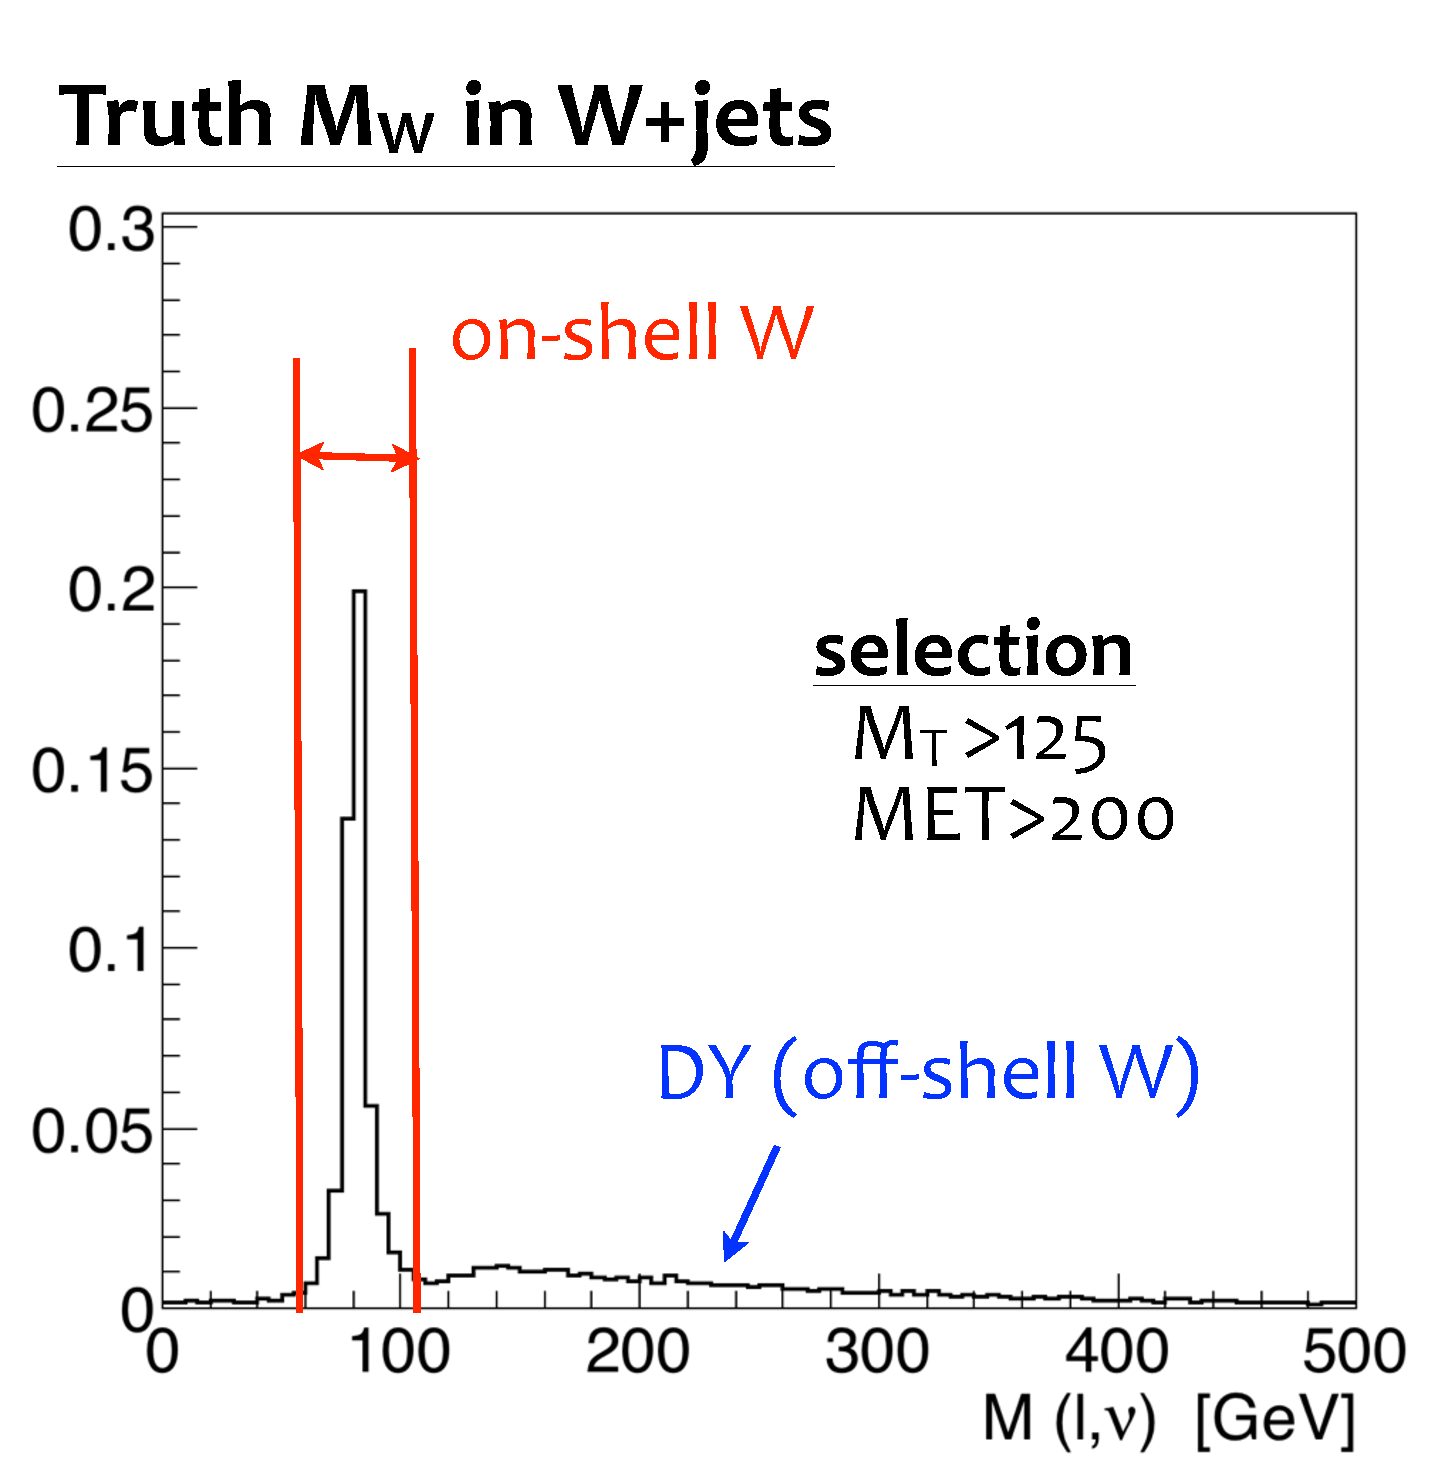
\includegraphics[width=0.415\textwidth]{figures/BGestimation/BGcomponent/Wmassline_mt125.pdf}}
    \subfigure[]{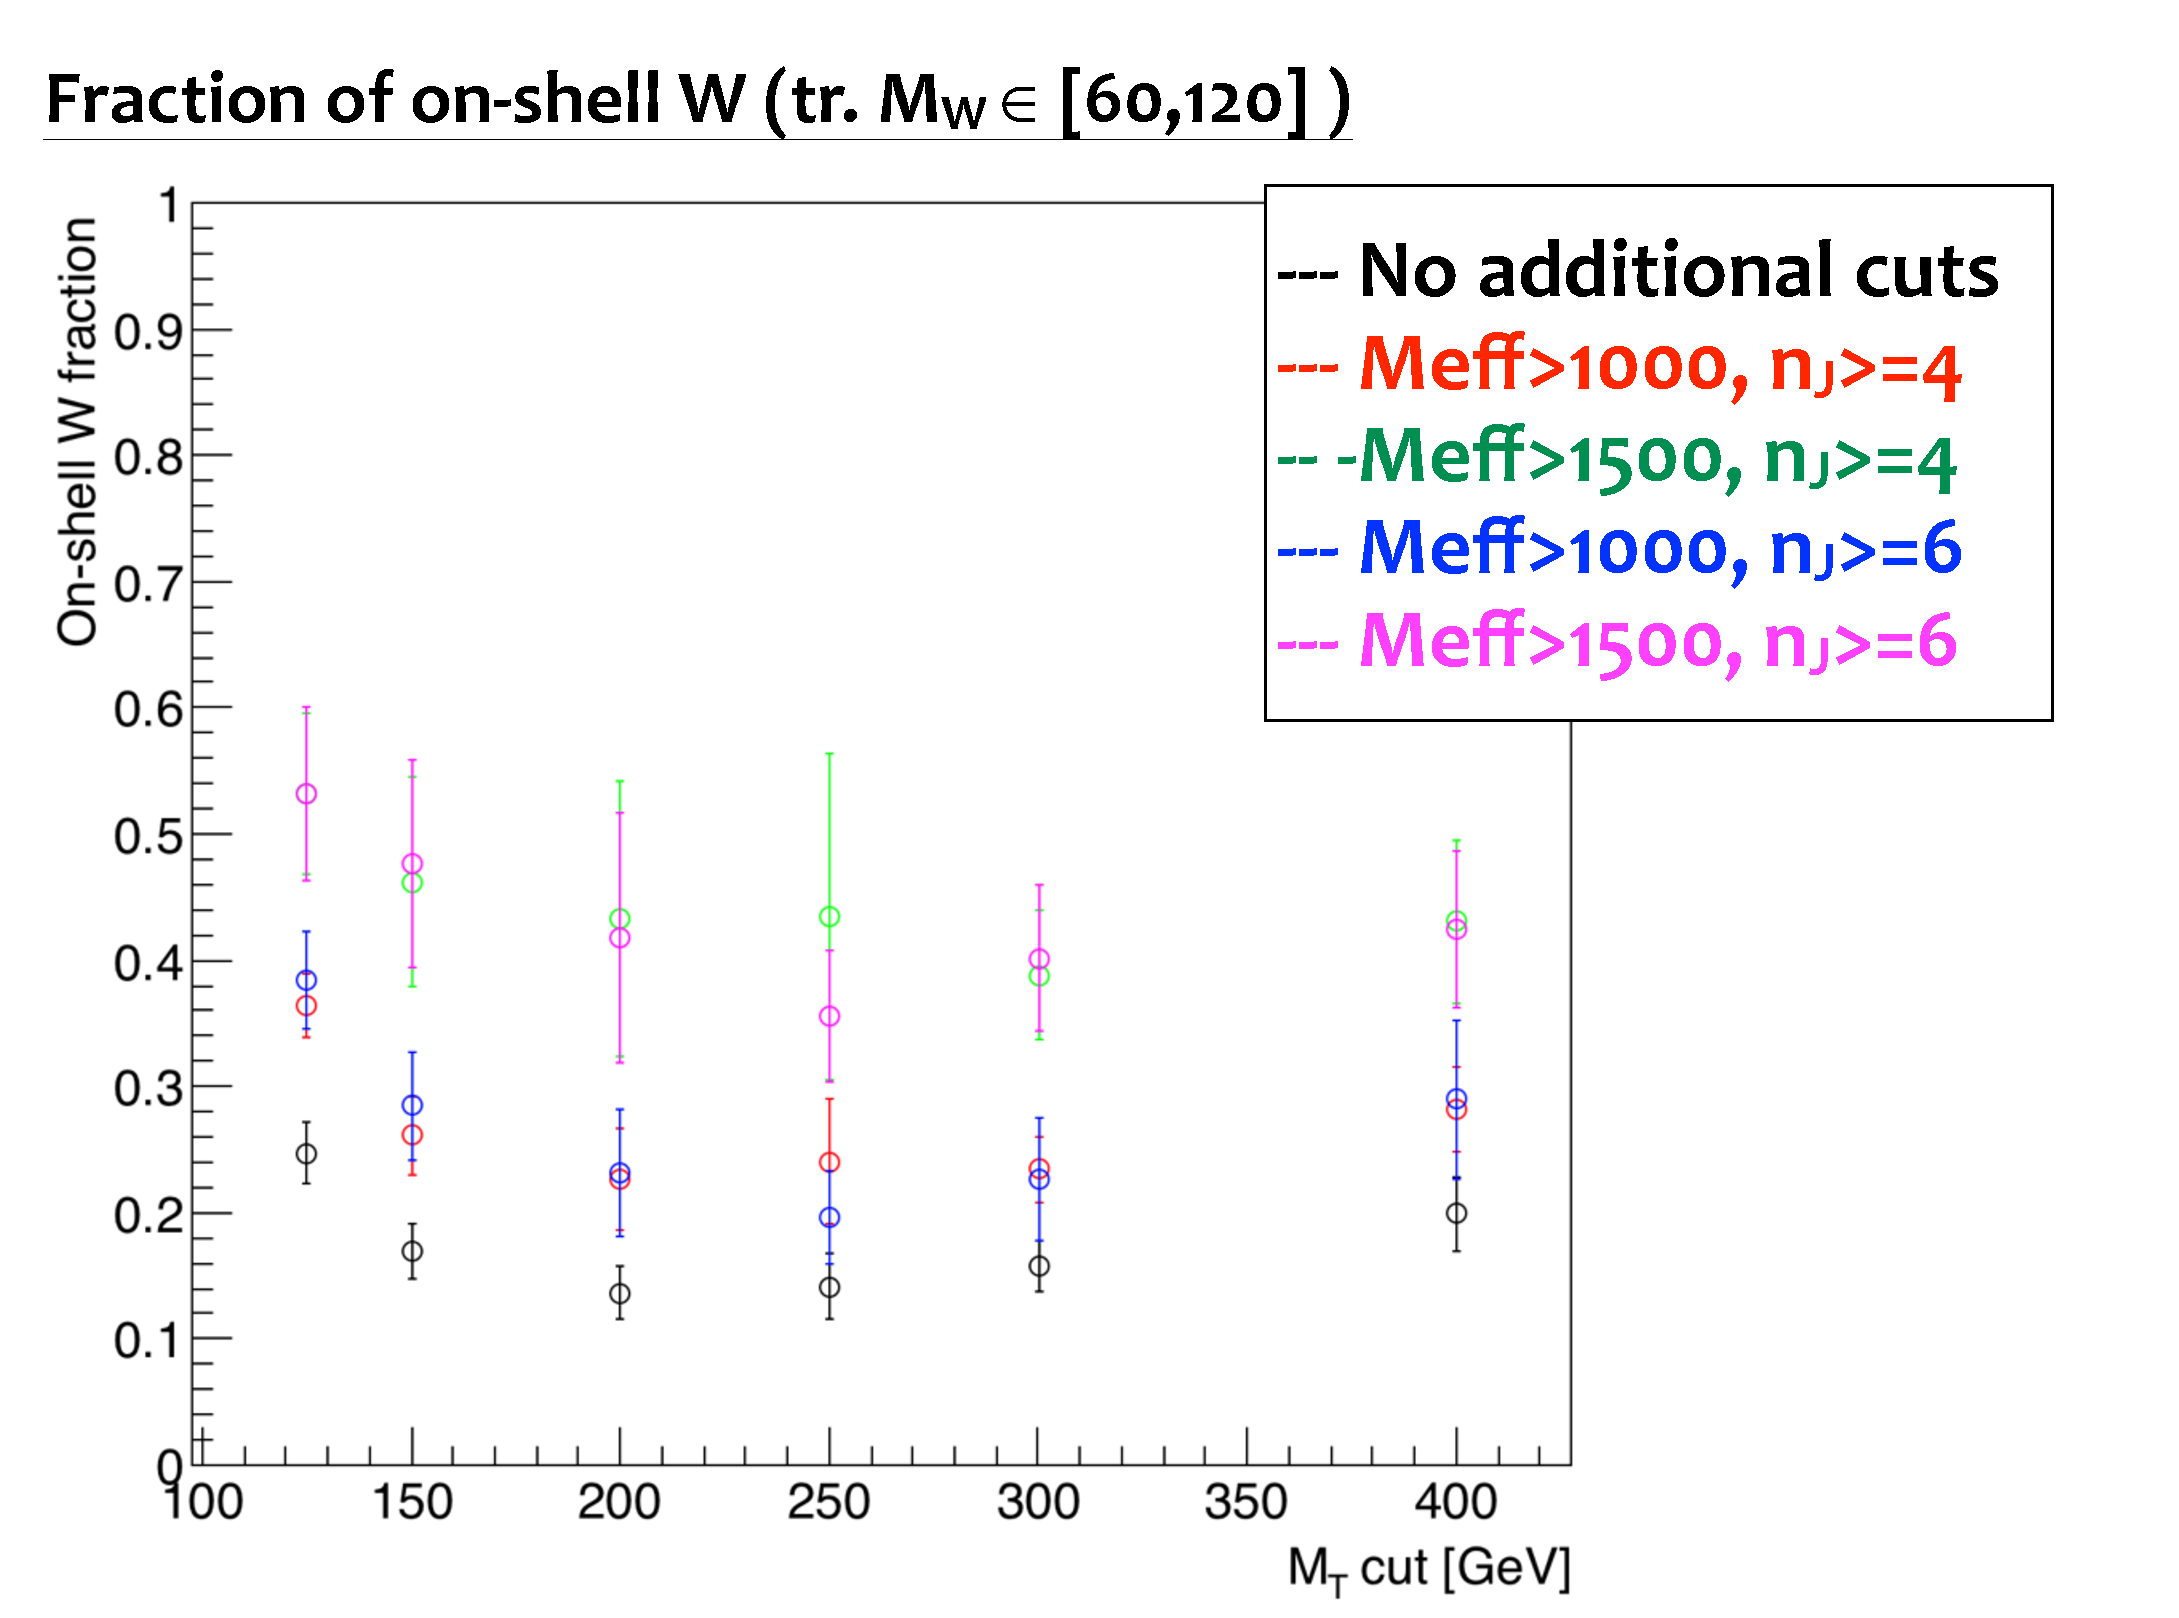
\includegraphics[width=0.575\textwidth]{figures/BGestimation/BGcomponent/Wjets_onshellFrac_highMT.pdf}}
    \caption{ (a) Truth invariance mass $m(\ell,\nu)$ of high-$\mt$ $\wjets$ events. Ideally there are only high-mass Drell-Yan type of events, however due to the finite detector resolution, a fraction of on-shell W events with badly measured MET sneak into regions with $\mt>m_W$. (b) The fraction of on-shell events defined by $m(\ell,\nu) \in [60,125]$, as a function of the $\mt$ cut. It is generally below 50 $\%$, however increases with higher jet activity in the event. \label{fig::BGestimation::Wmassline} }
\end{figure}
%%%%%%%%%%

The \textbf{``di-leptonic''} category consists of processes with real two leptons including $\tau$, mainly from di-leptonic decaying $\ttbar$, $Wt$ and $WW$. The presence becomes highly significant with respect to the ``semi-leptonic'' after the $\mt$ cut, since the source of missing transverse momentum is multiple thus they have no reason to cut-off at $m_{W}$.  \\
They fall into 1-lepton regions through two channels, namely ``$\ell\ell_{\mathrm{mis.}}$'': events with two real light flavor leptons and one of them fails the ``baseline'' requirement ("missing lepton"), and ``$\ell\tau_{\mathrm{h}}$'': events with a real light flavor lepton and a hadronically decaying tau lepton. \\
%
The origin of ``missing lepton'' is further four-fold and symbolized as follow: 
\begin{description}
\item [``Out Acc.''] \mbox{} \\
 Leptons going outside the acceptance of ``baseline'' requirement i.e. $p_{\mathrm{T}}>7(6)\gev, |\eta|<2.47(2.5)$ for electrons (muons).
\item [``Mis. Reco''] \mbox{} \\
 Leptons within the $\pt-\eta$ acceptance but failing the reconstruction i.e a truth lepton that can not be associated with any of reconstructed electrons/muons in the xAOD container.
\item [``Mis. ID''] \mbox{} \\
 Reconstructed leptons within the $\pt-\eta$ acceptance but failing the electron/muon ID for the ``baseline'' requirement.
\item [``Mis. OR''] \mbox{} \\
 Reconstructed leptons within the $\pt-\eta$ acceptance passing the ID for "baseline" requirement, but killed in the overlap removal (Sec. \ref{sec::objDef::OR}). 
%Technically, here it is defined as an identified lepton with the nearest non-b-tagged jet closer than $\Delta<0.4$.
\end{description}

One nice thing about this \textbf{``di-leptonic''} components is that 2-lepton regions are available for control regions in the estimation. Since no signal regions are set there, exactly the same phase space with respect to SRs can be exploited. This is performed by the ``object replacement method'' as detailed in the following sub-section, although ``Out Acc.'' and ``Mis. OR'' are challenging for some technical reasons thus are estimated altogether with the  \textbf{``semi-leptonic''} events. \\
%

The third category \textbf{``fake''} involves events with a fake lepton, which is negligible except regions dealing with soft leptons (\textbf{``2J''} and \textbf{``Low-x''}). Dominant contribution is from $W\ra\tau\nu$ and $Z\ra\nu\nu$ which accompanies a large MET from neutrinos. While the contribution from the multi-jets process is supposed to be negligible, it is dedicatedly cross-checked since the impact could be hazardous due to the huge cross-section. This is done using a series of validation regions referred as VRs-QCD, shown in Appendix \ref{sec::BGestimation::VRQCD}. \\
%(footnote) for definition of ``fake'' please refer Sec. \ref{sec::fakeLepton}.  

The relative popularity over the sub-categories in the signal regions are summarized in Figurere \ref{fig::BGestimation::BGcomposition_objRep} illustrates, where \textbf{``semi-leptonic''} and \textbf{``di-leptonic''} (particularly ``$\ell\tau_h$'') are overwhelmingly dominant in BV and BT signal regions respectively.


\clearpage
\begin{figure}[h]
  \centering
    \subfigure[]{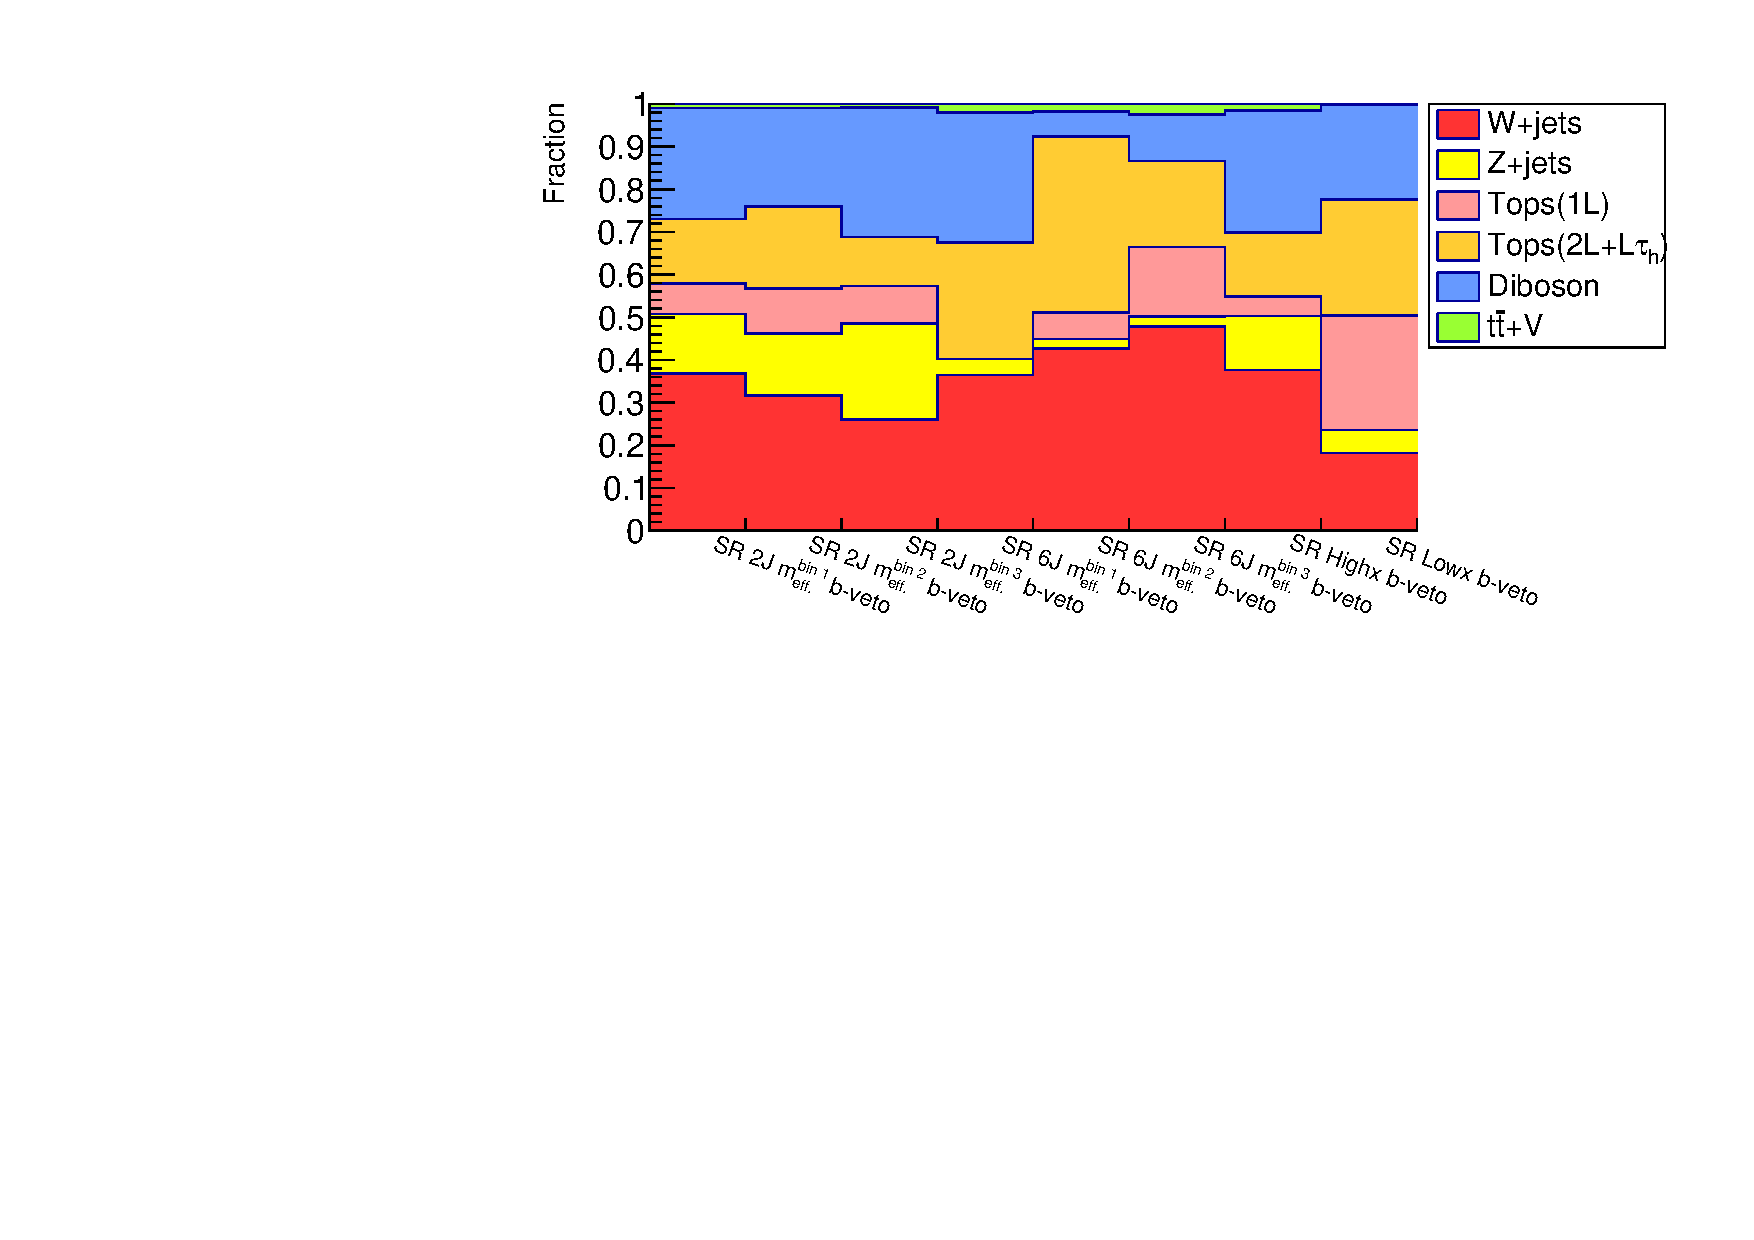
\includegraphics[width=0.97\textwidth]{figures/BGestimation/BGcomponent/prod-01-825-03/BGcomp_splitLv2_SRBV_norm.pdf}}
%    \subfigure[]{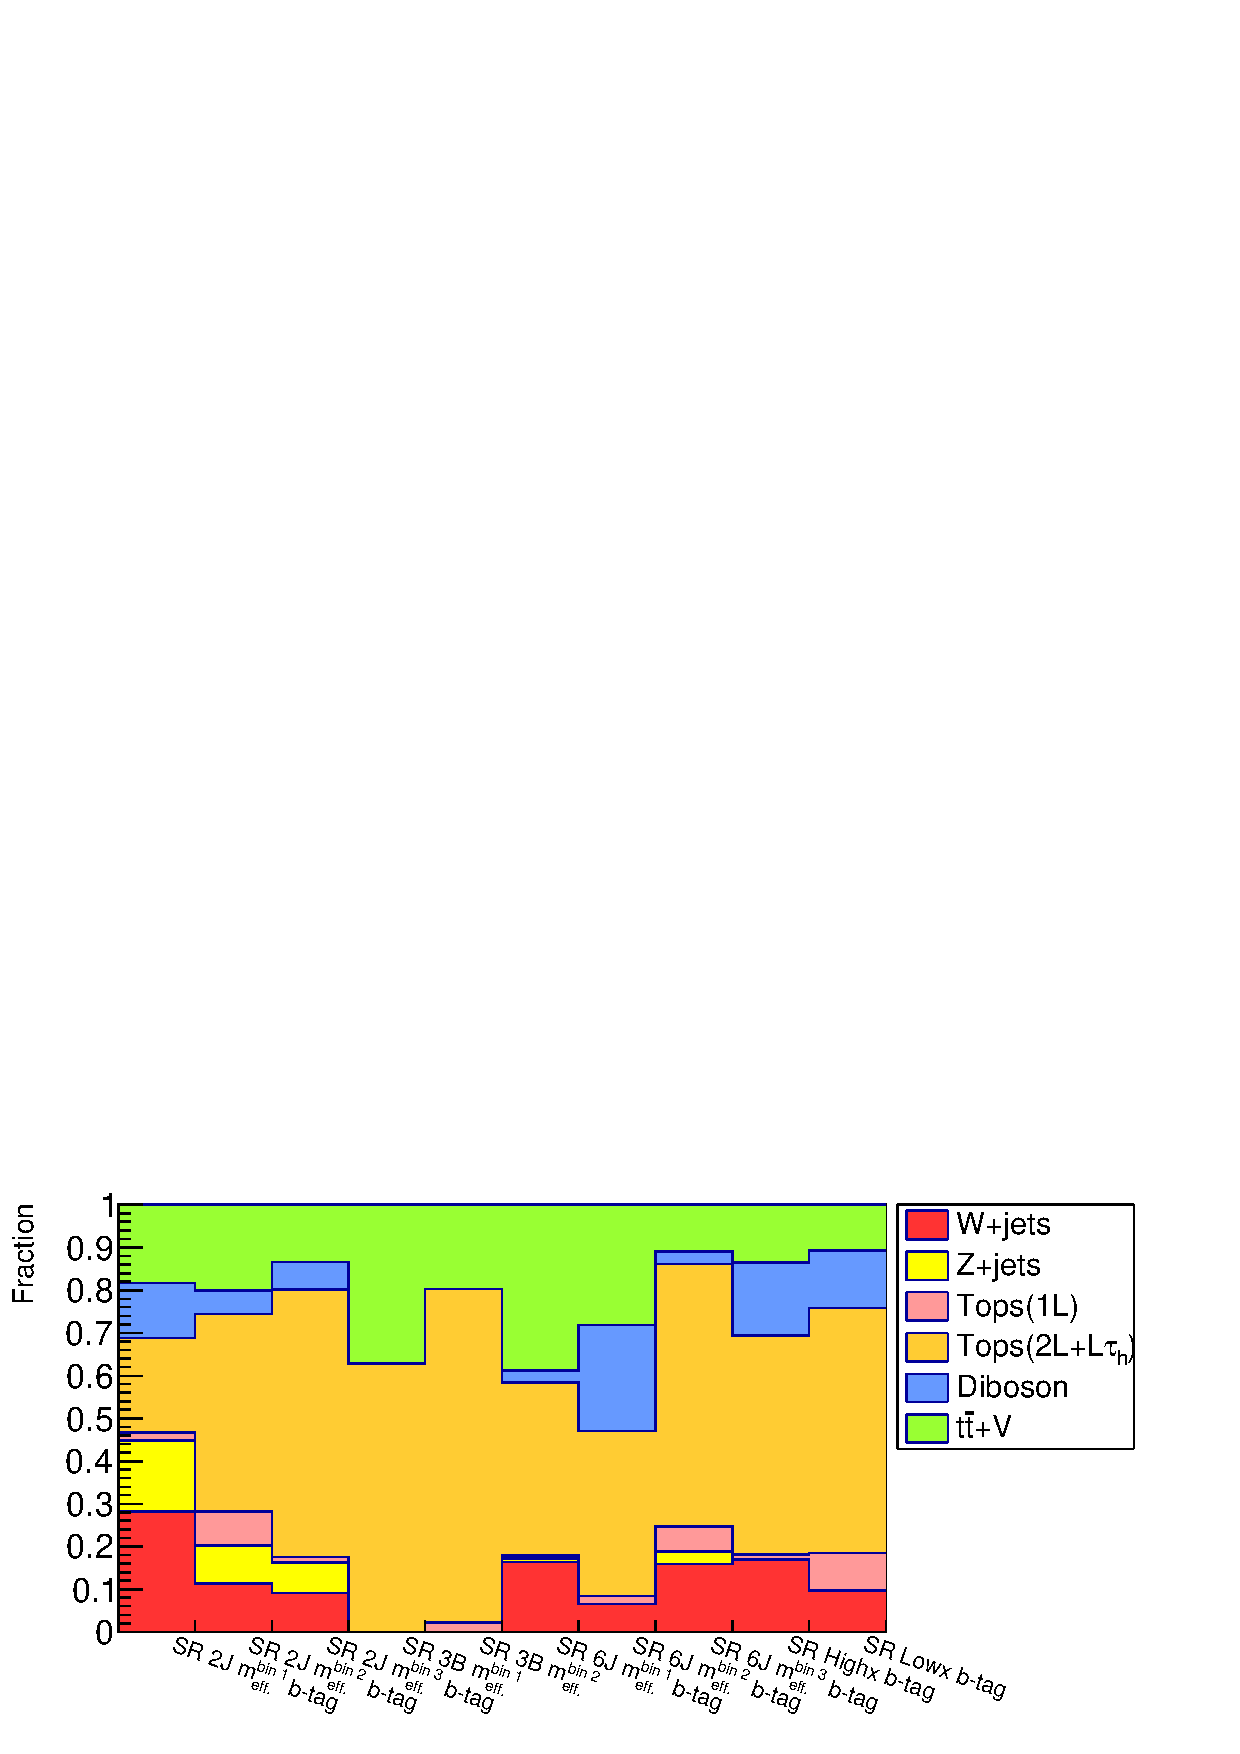
\includegraphics[width=0.97\textwidth]{figures/BGestimation/BGcomponent/prod-01-825-03/BGcomp_splitLv2_SRBT_norm.pdf}}
    \subfigure[]{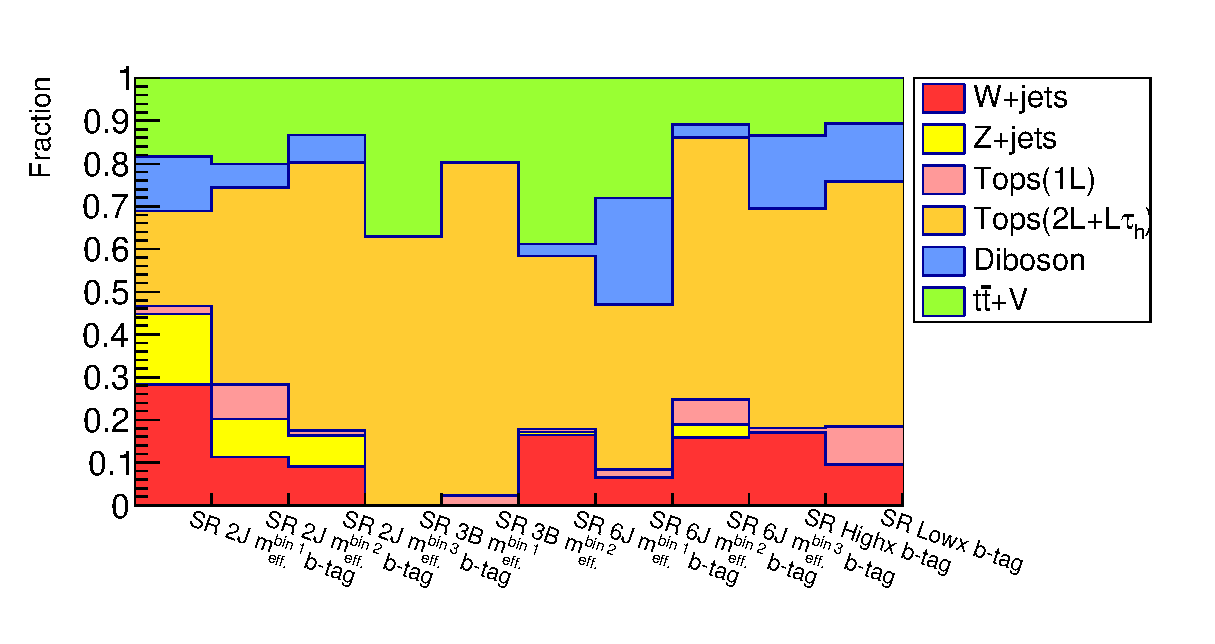
\includegraphics[width=0.97\textwidth]{figures/BGestimation/BGcomponent/prod-01-825-03/BGcomp_splitLv2_SRBT_norm.eps}}
    \caption{ Background composition in terms of physics processes in the (a) BV, and (b) BT/3B signal regions. $\ttbar$ and single-top are merged as ``Tops'', and the semi-leptonic and di-leptonic components are respectively labeled as ``semi-leptonic'' and ``$2L+L\tau_h$''. \label{fig::BGestimation::BGcomposition_splitLv2} }
\end{figure}

\clearpage
\begin{figure}[h]
  \centering
    \subfigure[]{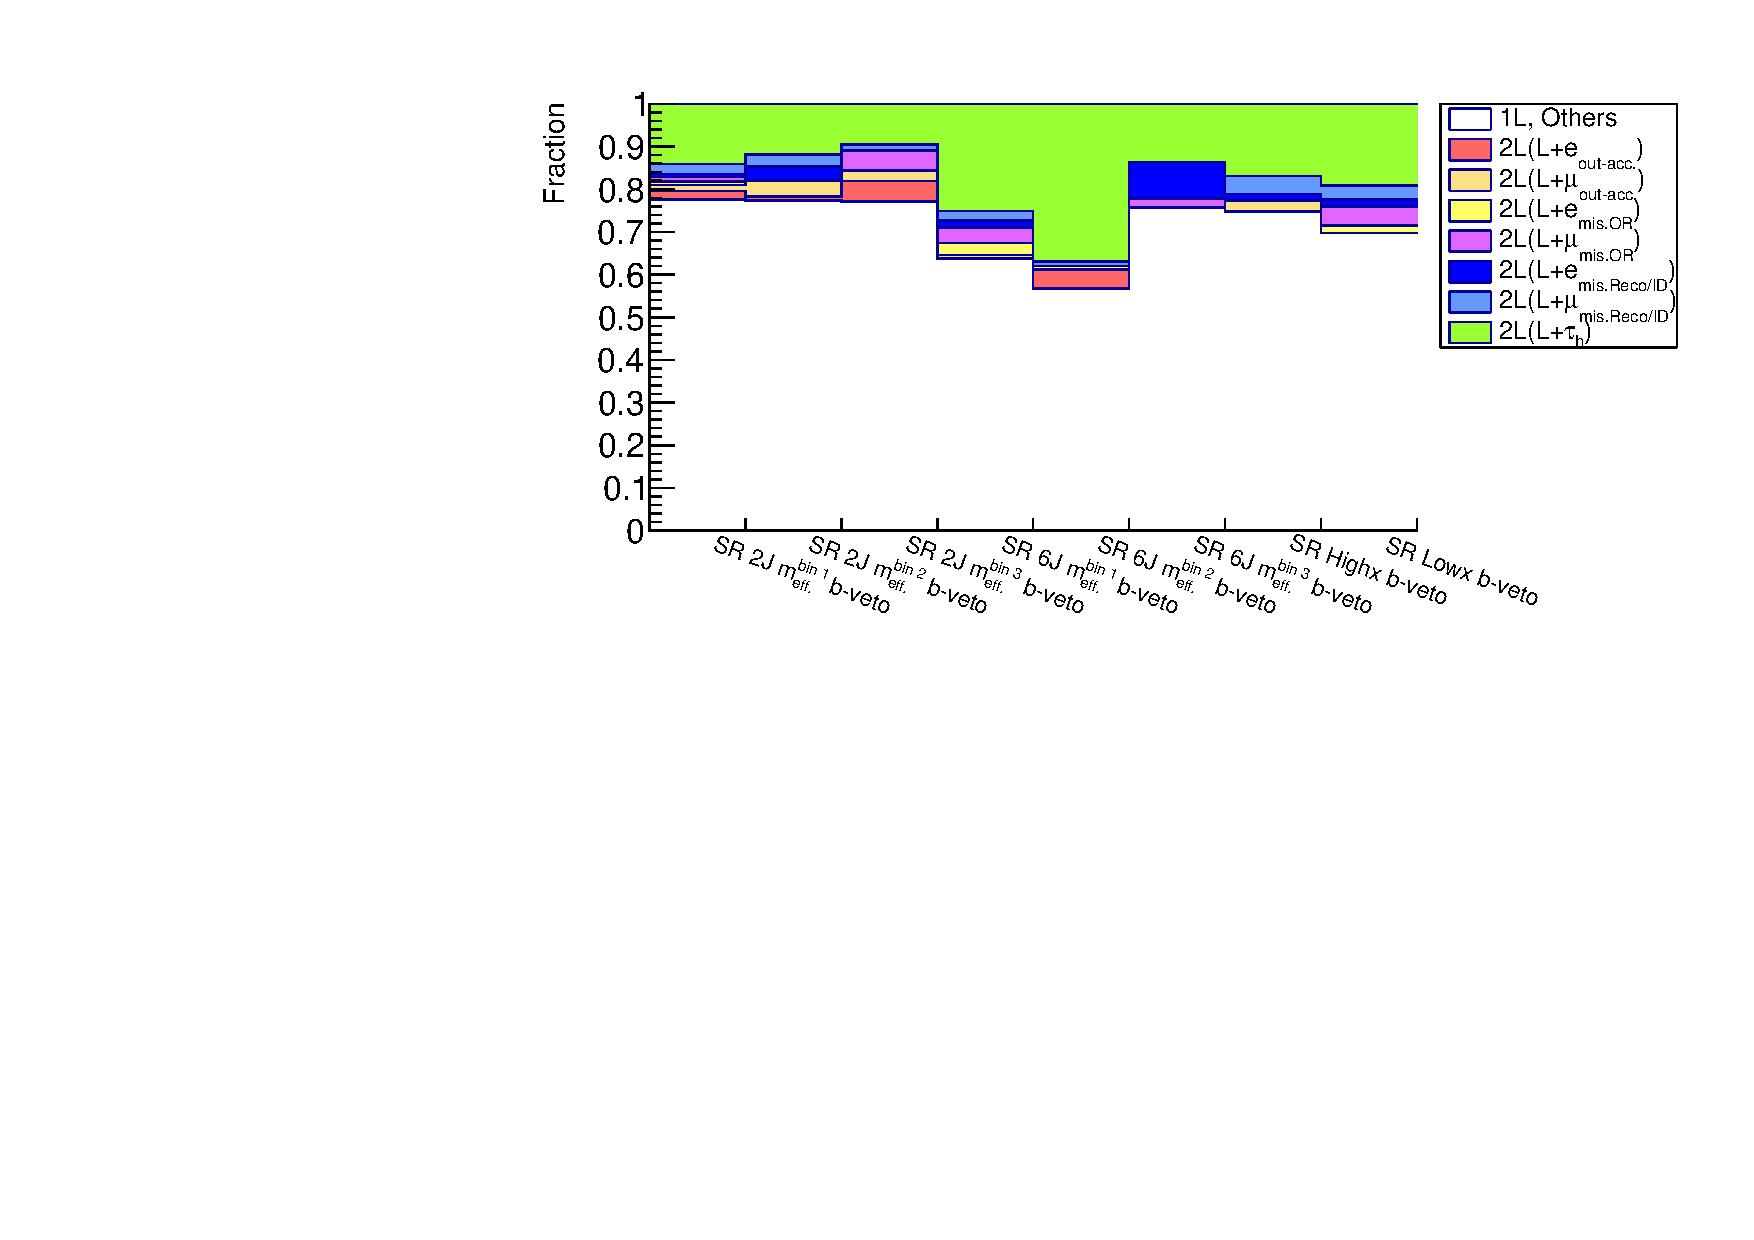
\includegraphics[width=0.97\textwidth]{figures/BGestimation/BGcomponent/prod-01-825-03/BGcomp_objRep_SRBV_norm.pdf}}
%    \subfigure[]{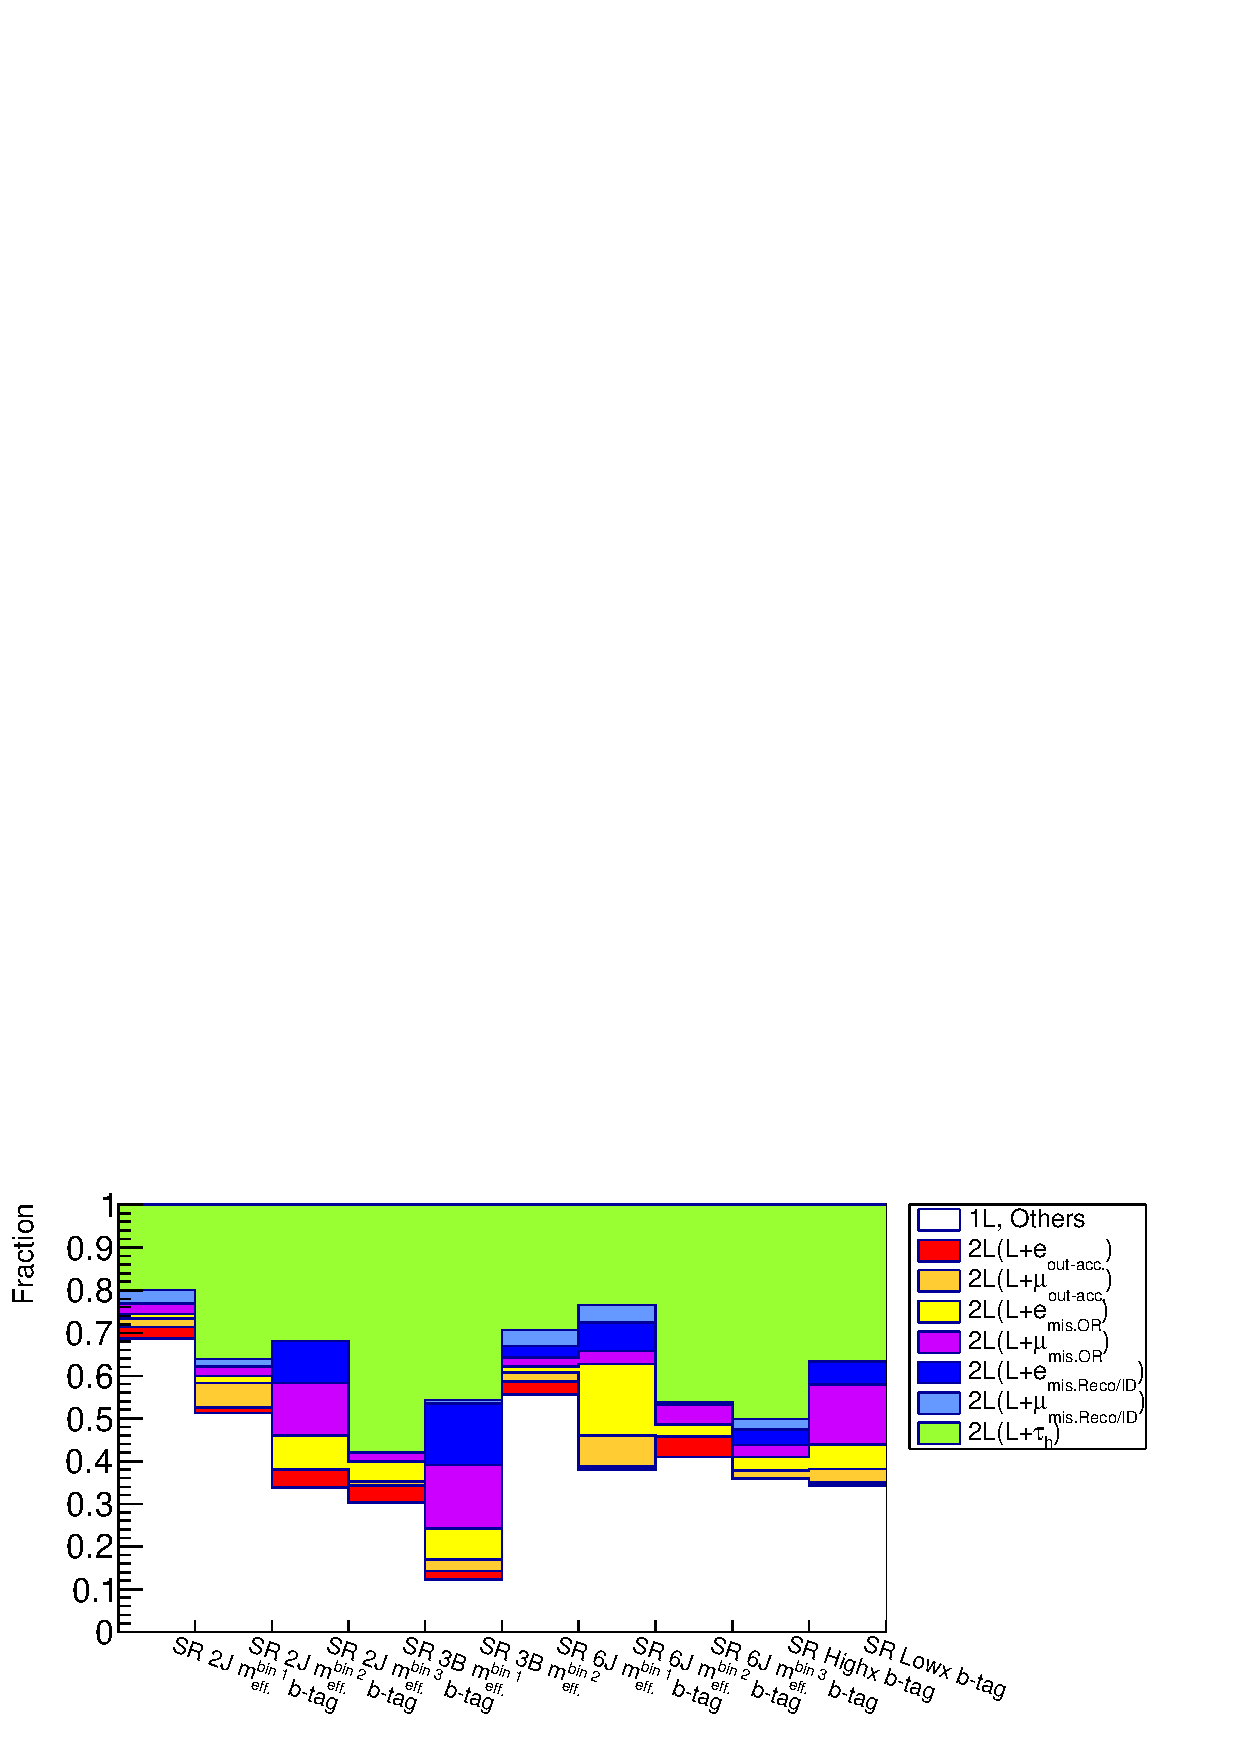
\includegraphics[width=0.97\textwidth]{figures/BGestimation/BGcomponent/prod-01-825-03/BGcomp_objRep_SRBT_norm.pdf}}
    \subfigure[]{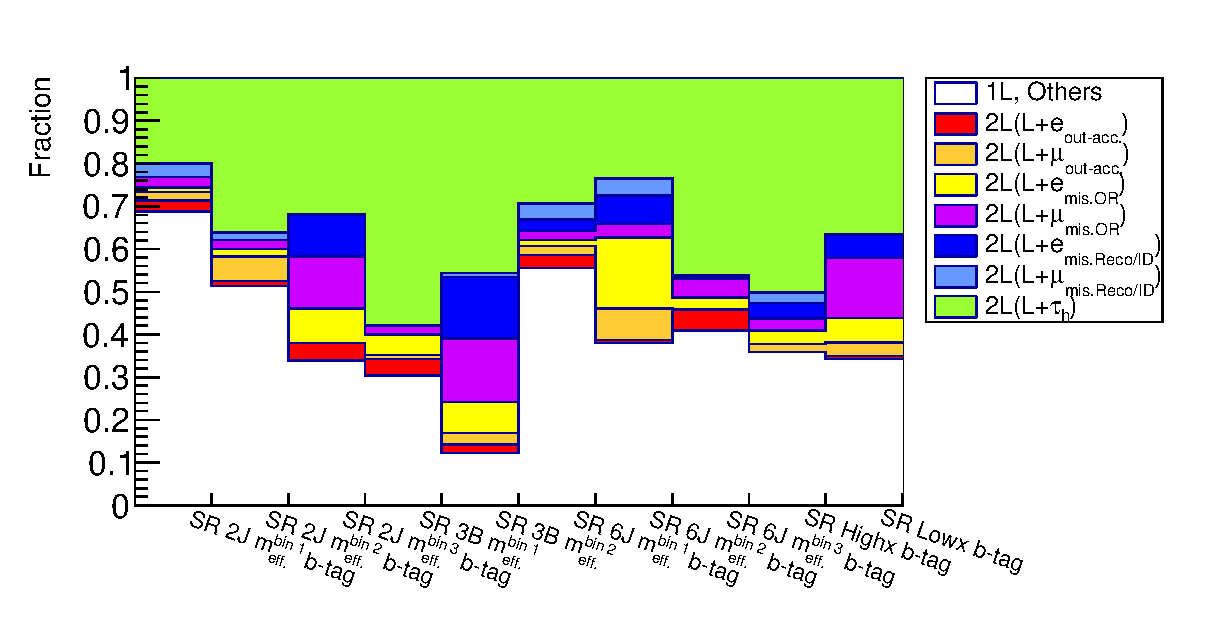
\includegraphics[width=0.97\textwidth]{figures/BGestimation/BGcomponent/prod-01-825-03/BGcomp_objRep_SRBT_norm.eps}}
    \caption{ Background breakdown in the (a) BV, and (b) BT/3B signal regions based on the classification in Table \ref{tab::BGestimation::BGclass}. While the BV signal regions are dominated by the ``semi-leptonic'' category, BT/3B signal regions are mainly with ``di-leptonic'' especially the ``$\ltauh$'' component.
 \label{fig::BGestimation::BGcomposition_objRep} }
\end{figure}


%%%%%%%%%%%%%%%%%%%%%%%%%%%%%%%%%%%
\clearpage


%%%%%%%%%%%%%%%%%%%%%%%%%%%%%%%%%%%
\subsection{The Kinematical Extrapolation Method} \label{sec::BGestimation::kineExtp}
The design of kinematical extrapolation method begins with control region definition.
It is basically a procedure where one specifies kinematical variables well-modeled by MC that are suitable for the extrapolation from control region (CR) to signal region (SR), and tuning the selection in those variables under a couple of rules and considerations. These are discussed in Sec. \ref{sec::BGestimation::dataMC} and Sec. \ref{sec::BGestimation::CRdef} respectively. While MC is normalized to data in the determied CRs, the most imporant thing is that the behavior (or the cause) of the MC mis-modeling is more or less understood. 
%What one should avoid is to have multiple sources of mis-modeling that contribute oppositely, leading to underestimation of mis-modeling.
Therefore, an extensive investigation in the MC mis-modeling modeling is simultaneously done in Sec. \ref{sec::BGestimation::dataMC}.  \\


\subsubsection{MC vs Data Comparison and the MC mis-modeling} \label{sec::BGestimation::dataMC}
The MC modeling of dominant background processes ($\wjets$ and $\ttbar$) is examined in pre-selection regions defined in Table\ref{tab::BGestimation::preselectionDef}. Each pre-selection region is intended to be dominated by the process being tested. 

\tab{c|c|c|c|c|c}{
  \hline
  Region name            & $\nLepbase$ & $\nLepsignal$ & $\lepOnePt$ [GeV]     & $\nBJet$  & Tested processes   \\
  \hline
  \hline
%  1L   (hardLep/softLep) & 1           & 1             & $>35$ / $[7(6),35]$ for $e$ ($\mu$) & -        & $\wjets$, $\ttbar$ \\
  1LBV (hardLep/softLep) & 1           & 1             & $>35$ / $[7(6),35]$ for $e$ ($\mu$) & $0$      & $\wjets$           \\
  1LBT (hardLep/softLep) & 1           & 1             & $>35$ / $[7(6),35]$ for $e$ ($\mu$) & $[1,2]$  & $\ttbar$           \\
  2LBT                   & 2           & 2             & -                     & $[1,2]$  & $\ttbar$           \\ 
  1L3B                   & 1           & 1             & $>15$                 & $\geq 3$ & $\ttbar+cc/bb$, $\ttbarFakeB$ \\
  \hline
}
{Definition of pre-selection regions and corresponding tested physics processes. MET trigger requirement, event cleaning described Sec. \ref{sec::SRdefinition::eventCleaning}, $\nJetNoGev \geq 2$ and $\met>250$ are applied as common selection.}
{tab::BGestimation::preselectionDef}

\paragraph{$\bf{\wjets}$}
Figurere \ref{fig::BGestimation::DataMCPreselHardBV1} - \ref{fig::BGestimation::DataMCPreselHardBV2} show the kinematic distribution of the pre-selection region \textbf{1LBV hardLep} where $\wjets$ is enriched. While the bulk phase space is well-described by MC, there are a strking tendency of overestimation by MC in the tail. Discrepancy is mainly observed in distributions related to the jet activity, particularly in jet multiplicity when it is above 3. Considering that they here are all from ISRs or FSRs, and that the jet multiplicity in the event roughly corresponds to the number of QCD-order of the processes, this directly implies the mis-modeling in higher order effects beyond next-to-next-to-leading order (NNLO) level. This might not be surprising giving that the MC sample (Sherpa 2.2.1 generator) does not include loop diagrams beyond NLO and neither diagrams with more than 5 partons in the final state, due to computational limitation. \\

Therefore, an order-by-order cross-section correction should be helpful as the first aid. In fact, a simple MC reweighting in terms of jet multiplicity turns to work quite nicely. The reweighting function is derived by fitting linearly the observed data/MC in Figurere \ref{fig::BGestimation::DataMCPreselHardBV1} (a):
\begin{equation}
w = 1 - 0.1 \times (\nJetNoGev-2) \label{eq::BGestimation::rwgt_nJ},
\end{equation}
where $\nJetNoGev$ is the number of jets with transverse momenta greater than $30\gev$. While the jet multiplicity distribution is fully corrected by construction, the other discrepancies can be resolved almost perfectly as well, as shown in \ref{fig::BGestimation::DataMCPreselHardBV_rwgt1}. \\

Anthoer observed aspect of the mis-modeling is that it is more striking in terms of soft radiations rather than the hard ones. For example, the average jet transverse momentum distribution (Figurere \ref{fig::BGestimation::DataMCPreselHardBV_rwgt1} (c)) is well-modeled above $\sim 200 \gev$, while the slope of data over the MC for jet multiplicity distribution is rather persistent. This in fact backups that reweighting in other mis-modeled variables than jet multiplicity, such as $\meffInc$, actually does not work as successfully, since their tails are basically determined by hard jets. \\

Although this simple linear $\nJetNoGev$ reweighting demonstrated above seems qualitatively reasonable, it is not seriously used as correction due to the technical drawbacks that the optimum coefficients in Eq. \ref{eq::BGestimation::rwgt_nJ} has slight phase space dependence, and that it is difficult to validate them around signal regions since the data statistics is limited. However, it is still a good enough approximation as well as a useful reference expression to understand the behavior and correlation of mis-modeling between variables. The reweighting with Eq. \ref{eq::BGestimation::rwgt_nJ} is then used for emulating the mis-modeling when designing the data-driven background estimation as described in the following sub-sections. \\

Variables that do not scale with transverse momenta of outgoing particles, such as $\mt$ or $\apl$, keep relatively well-modeled up to the tails. Particularly, $\mt$ is by construction insensitive to most of the kinamtics since the tail is determied by the mass-line of $W$-boson and MET resolution. $\apl$ is also supposed to tbe robust by itself since it takes a form of ratio of jet momentum. Therefore, these variables are decided to be used for the extrapolation from control regions to signal regions. Note that the $\mt$ cut-off ($\mt \sim m_W$) is slightly mis-modeled typically when tigher selections are applied, presumably due to the simplified treatment of the mass-line in calculating diagrams with many additional partons. The effect becomes visible especially in CR (e.g. Figurere \ref{fig::BGestimation::CRpostFit::WRVarx}) and b-vetoed SRs.
%The effect becomes visible in validation regions and giving systematical upward pulls by about 1$\sigma$ (Figurere \ref{fig::BGestimation::VRPulls}). \\



\clearpage
%%%%%%%%%%%%%
\begin{figure}[h]
  \centering
    \subfig{0.46}{figures/BGestimation/DataMCComparison/Preselection_hardLepBV/nJet30__Preselection_hardLepBV.pdf}{Jet multiplicity}
    \subfig{0.46}{figures/BGestimation/DataMCComparison/Preselection_hardLepBV/jet1Pt__Preselection_hardLepBV.pdf}{$\pt$ of the leading jet}
    \subfig{0.46}{figures/BGestimation/DataMCComparison/Preselection_hardLepBV/averageJetPt__Preselection_hardLepBV.pdf}{Average $\pt$ of jets with $\pt>30\gev$}
    \subfig{0.46}{figures/BGestimation/DataMCComparison/Preselection_hardLepBV/meffInc30__Preselection_hardLepBV.pdf}{$\meffInc (\meffDef)$}
    \caption{ Kinematical distribution of data (black dots) and MC (colored stack) in the \textbf{1LBV} pre-selection region.  \label{fig::BGestimation::DataMCPreselHardBV1} }
\end{figure}

\begin{figure}[h]
  \centering
    \subfig{0.48}{figures/BGestimation/DataMCComparison/Preselection_hardLepBV/lep1Pt__Preselection_hardLepBV.pdf}{Lepton's $\pt$}
    \subfig{0.48}{figures/BGestimation/DataMCComparison/Preselection_hardLepBV/met__Preselection_hardLepBV.pdf}{$\met$}
    \subfig{0.48}{figures/BGestimation/DataMCComparison/Preselection_hardLepBV/mt__Preselection_hardLepBV.pdf}{$\mt$}
    \subfig{0.48}{figures/BGestimation/DataMCComparison/Preselection_hardLepBV/LepAplanarity__Preselection_hardLepBV.pdf}{$\Apl$}
    \caption{ Kinematical distribution of data (black dots) and MC (colored stack) in the \textbf{1LBV} pre-selection region.  \label{fig::BGestimation::DataMCPreselHardBV2} }
\end{figure}


%%%%%%%%%%%%%
\begin{figure}[h]
  \centering
    \subfigure[]{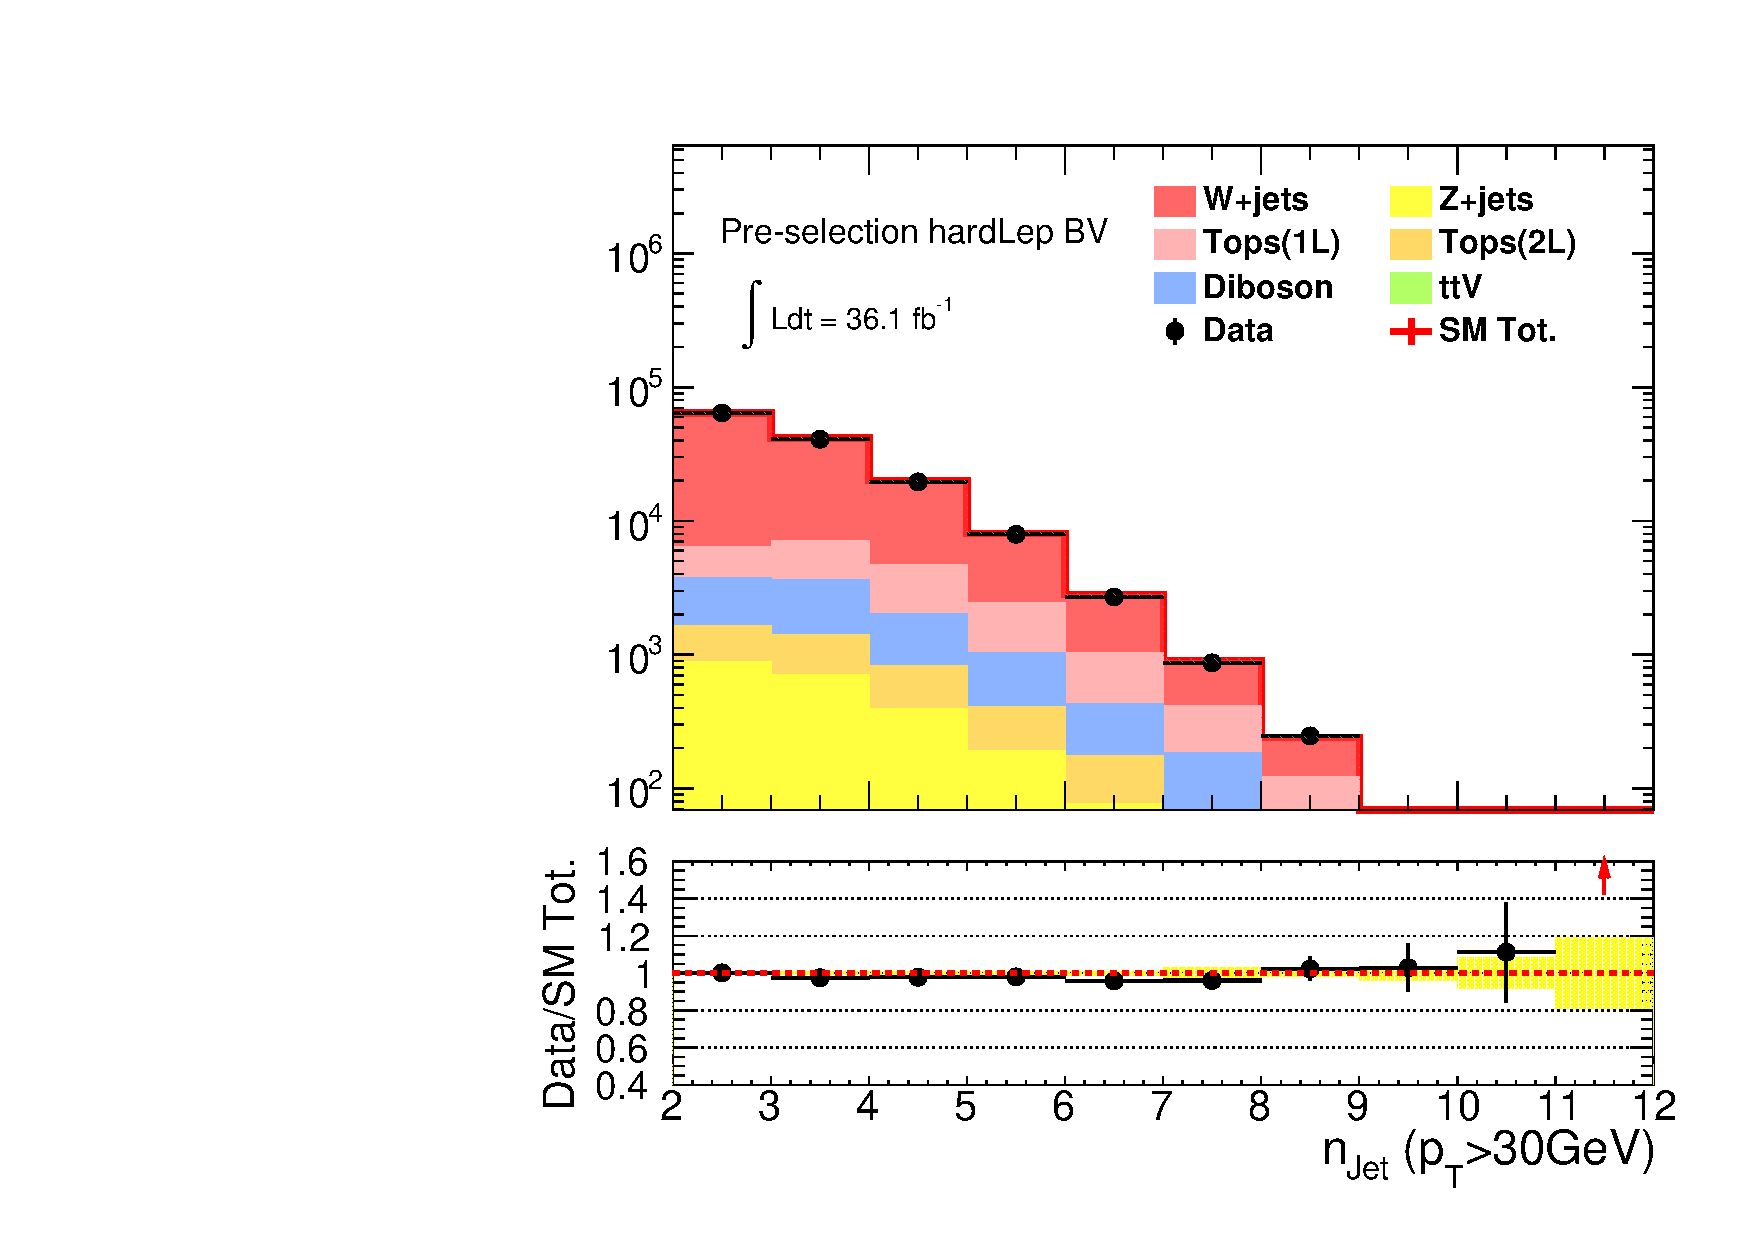
\includegraphics[width=0.48\textwidth]{figures/BGestimation/DataMCComparison/Preselection_hardLepBV/nJet30__Preselection_hardLepBV__rwgt_nJ007_ttPt007.pdf}}
    \subfigure[]{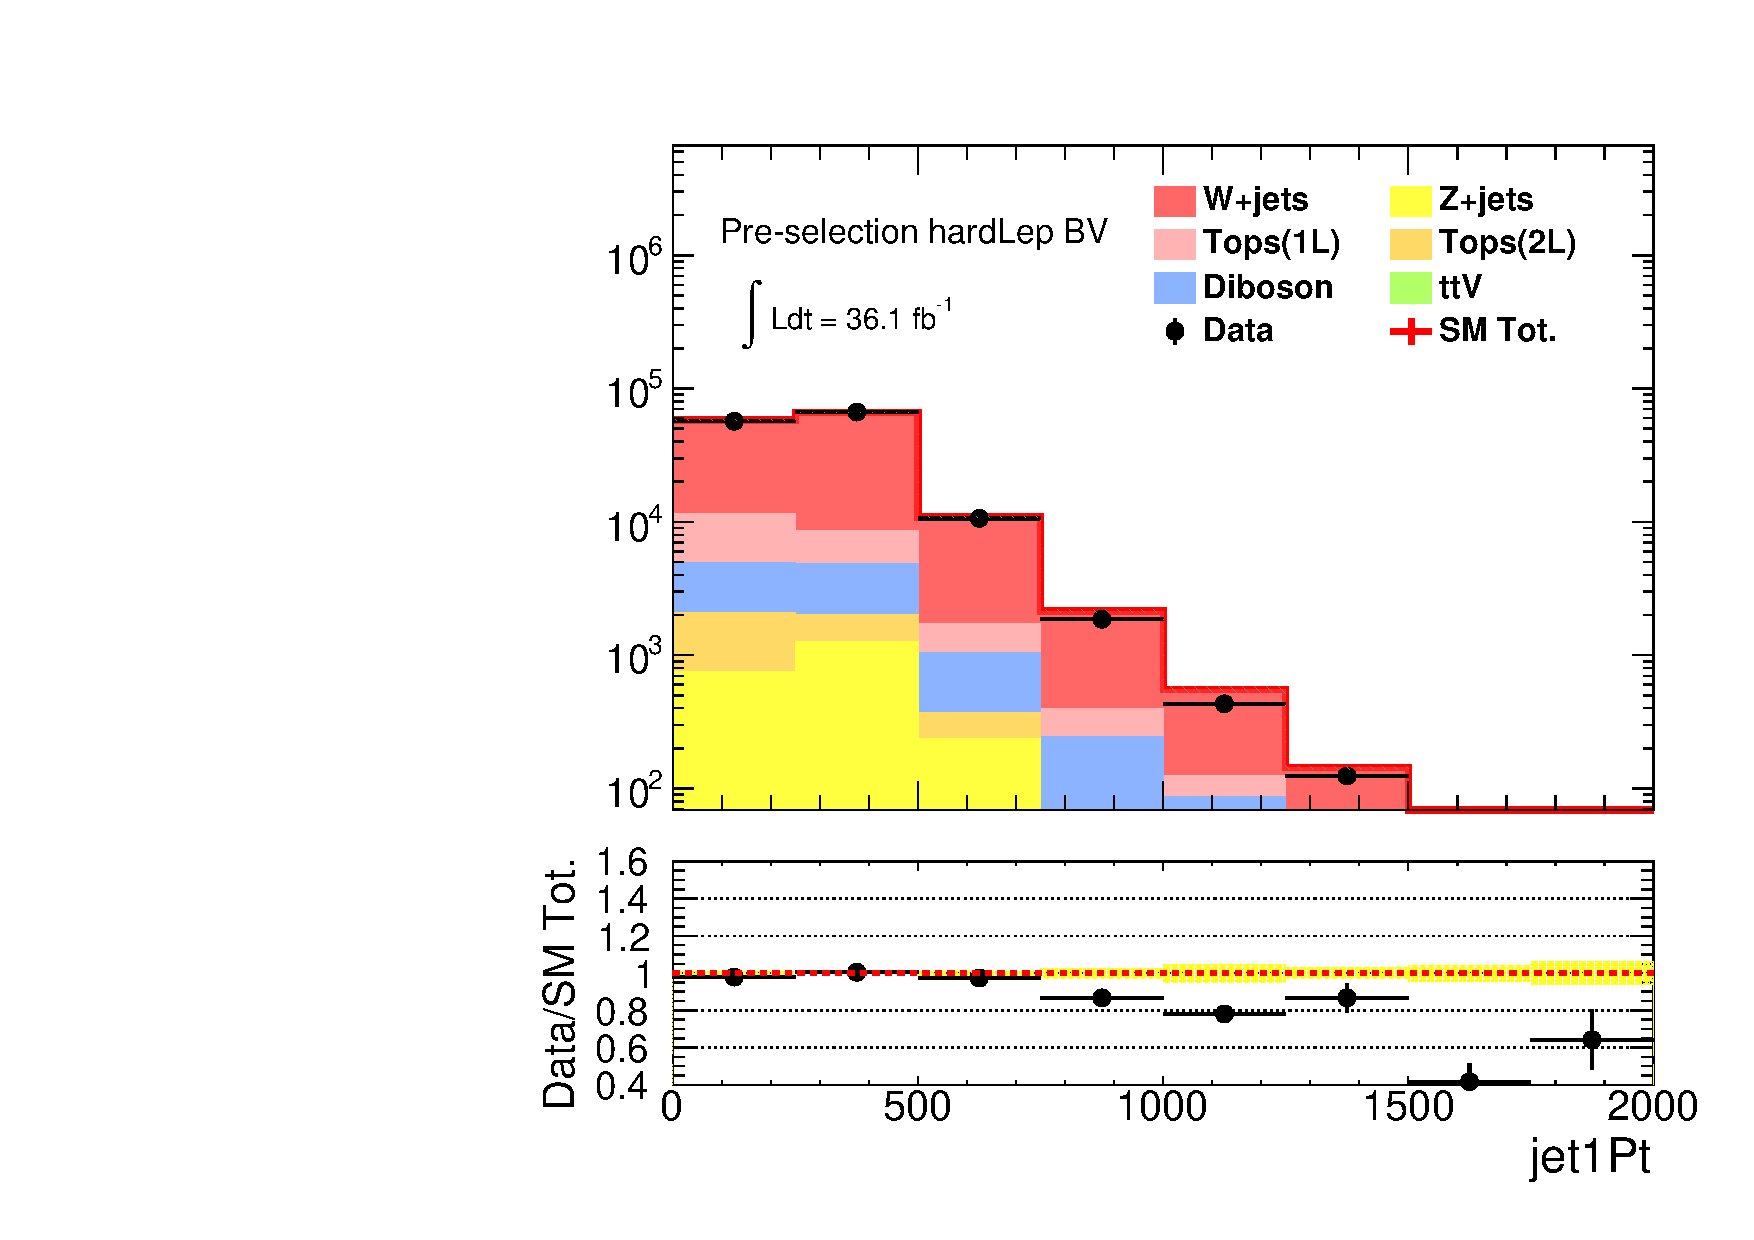
\includegraphics[width=0.48\textwidth]{figures/BGestimation/DataMCComparison/Preselection_hardLepBV/jet1Pt__Preselection_hardLepBV__rwgt_nJ007_ttPt007.pdf}}
    \subfigure[]{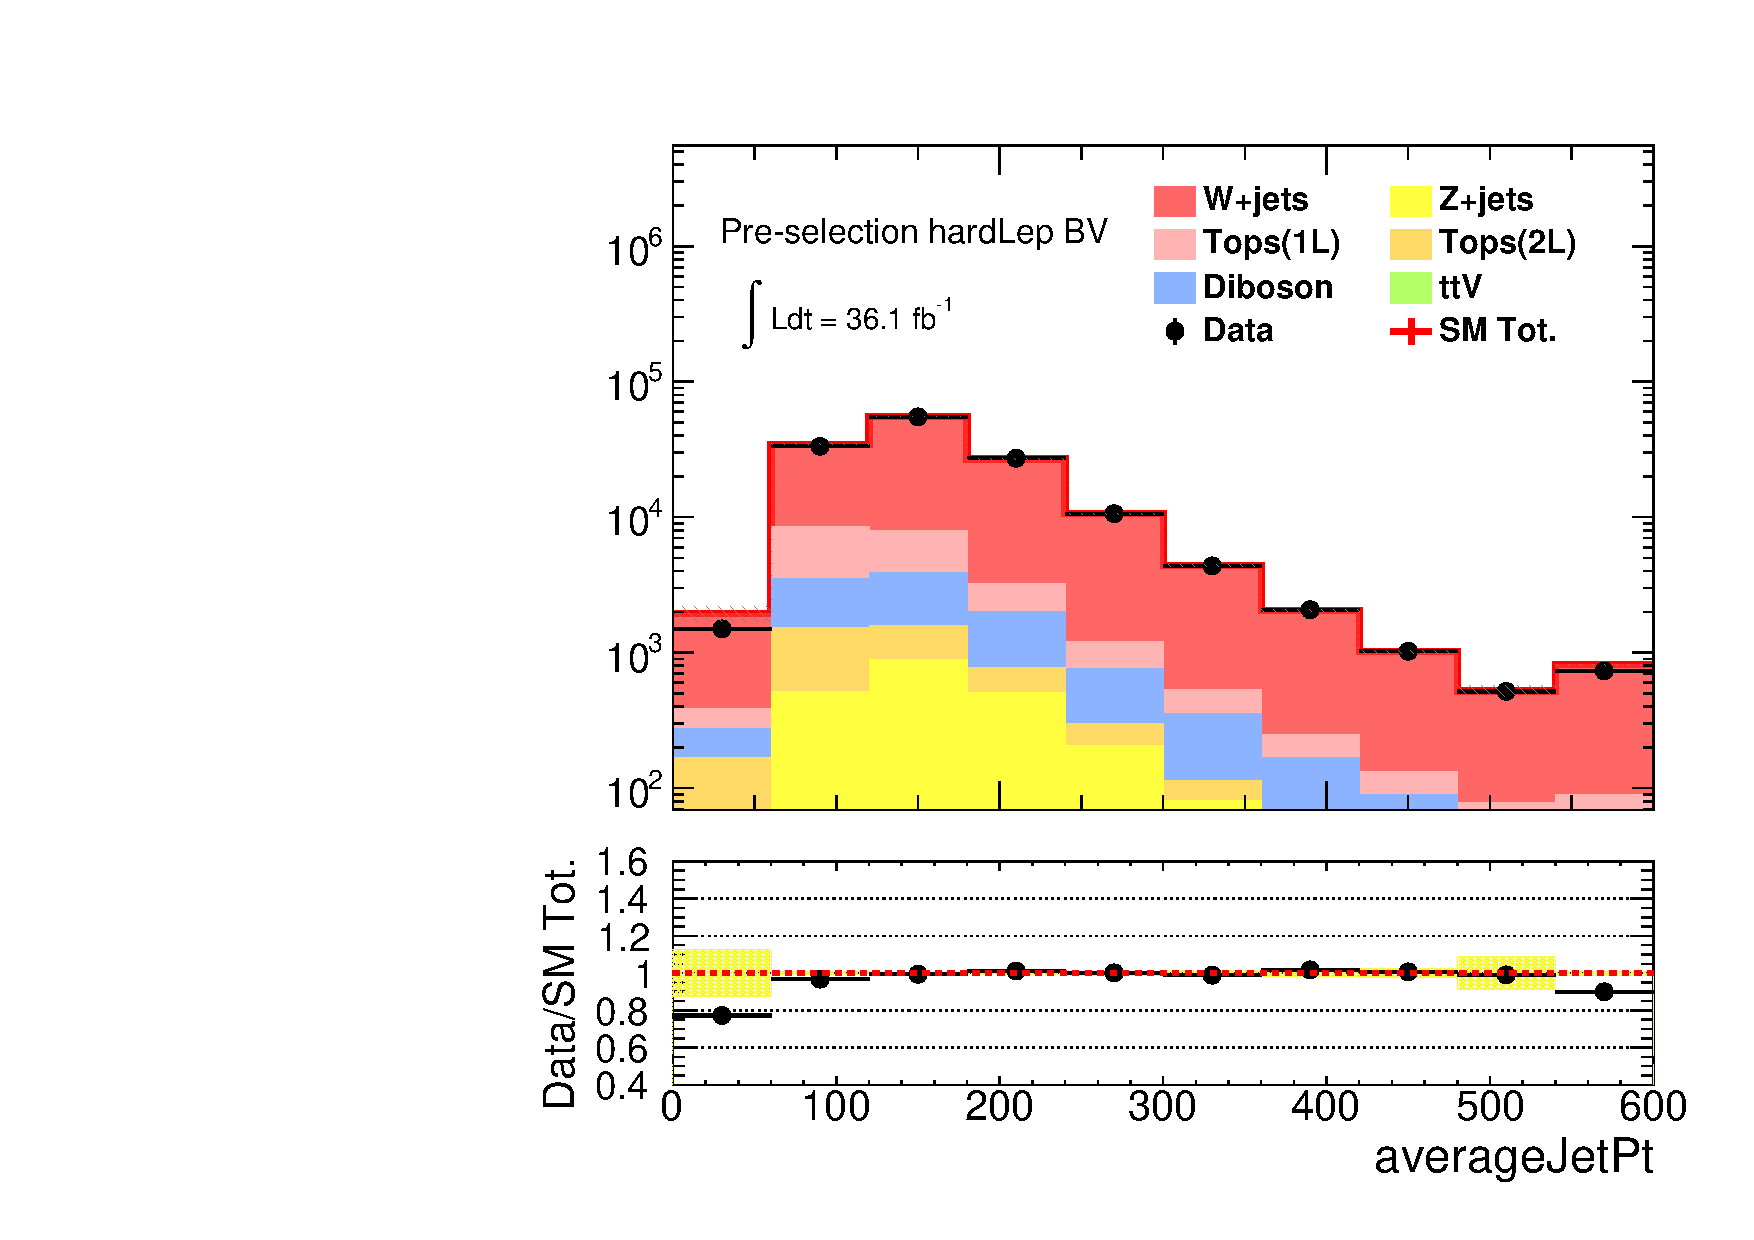
\includegraphics[width=0.48\textwidth]{figures/BGestimation/DataMCComparison/Preselection_hardLepBV/averageJetPt__Preselection_hardLepBV__rwgt_nJ007_ttPt007.pdf}}
    \subfigure[]{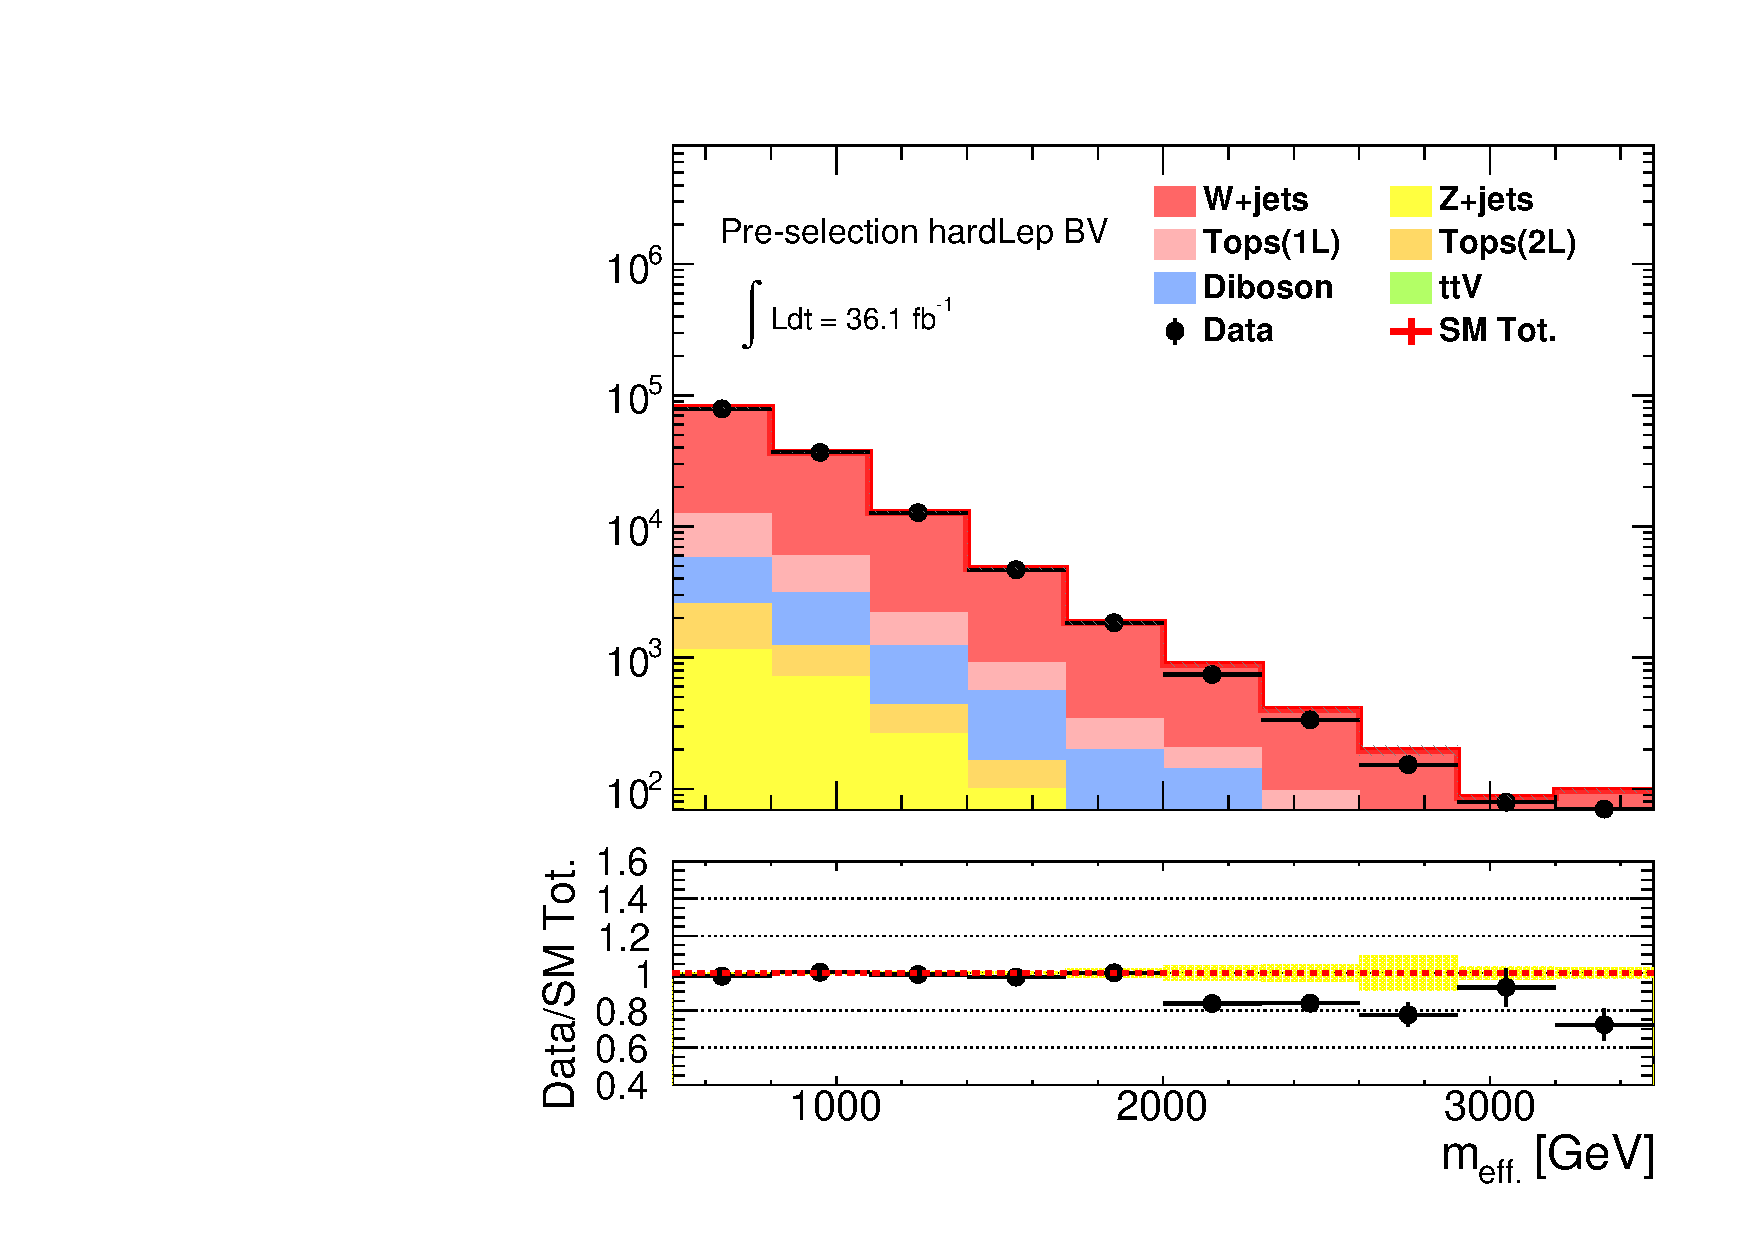
\includegraphics[width=0.48\textwidth]{figures/BGestimation/DataMCComparison/Preselection_hardLepBV/meffInc30__Preselection_hardLepBV__rwgt_nJ007_ttPt007.pdf}}
    \caption{ Kinematical distribution of (a) Jet multiplicity ($p_T>30\gev$) (b) leading-jet pt  (c) average jet pt ($p_T>30\gev$)  (d) $\meffInc$ in the hard lepton b-vetoed pre-selection region, with the reweighting $w = 1 - 0.1 \times (\nJetNoGev-2)$ (Eq.(\ref{eq::BGestimation::rwgt_nJ})) being applied for $\wjets$ MC. 
 \label{fig::BGestimation::DataMCPreselHardBV_rwgt1} }

\end{figure}

\begin{figure}[h]
  \centering
    \subfigure[]{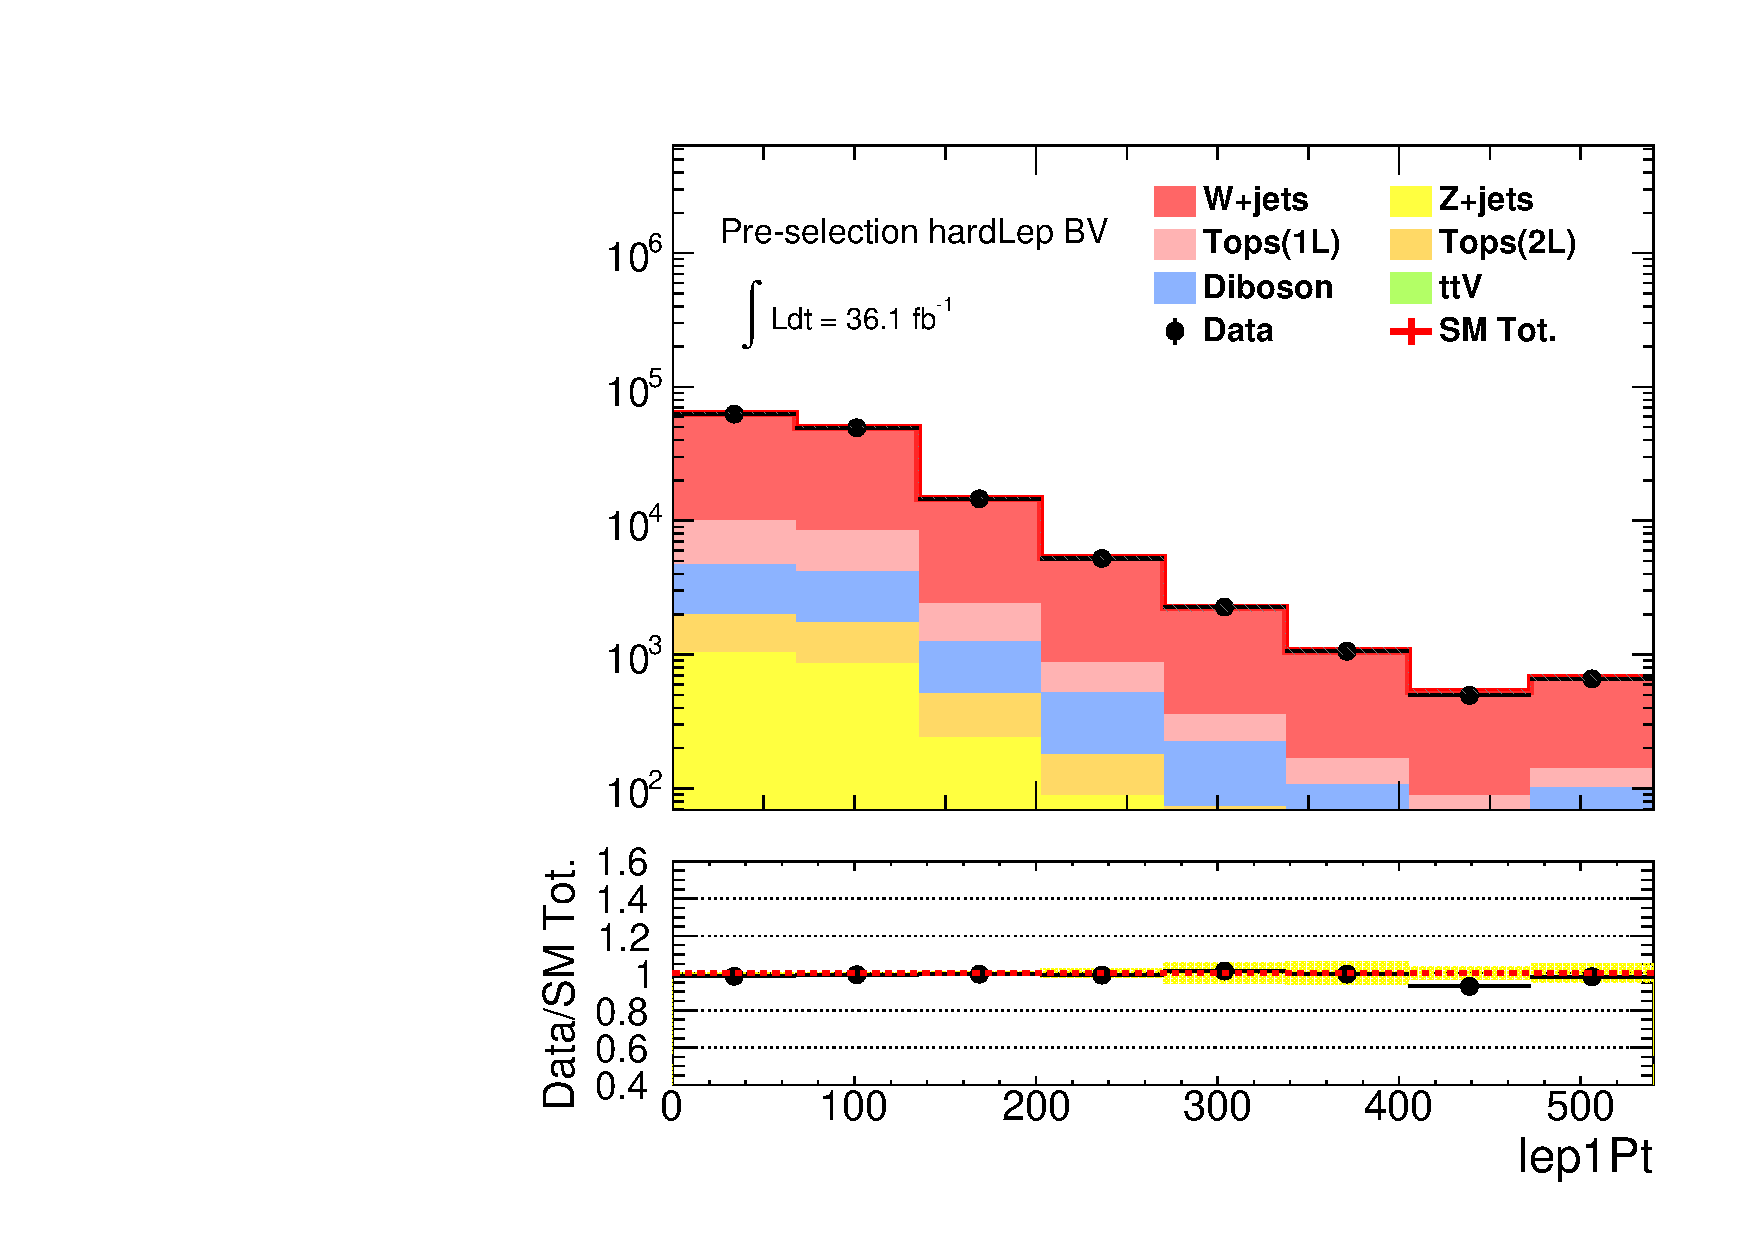
\includegraphics[width=0.48\textwidth]{figures/BGestimation/DataMCComparison/Preselection_hardLepBV/lep1Pt__Preselection_hardLepBV__rwgt_nJ007_ttPt007.pdf}}
    \subfigure[]{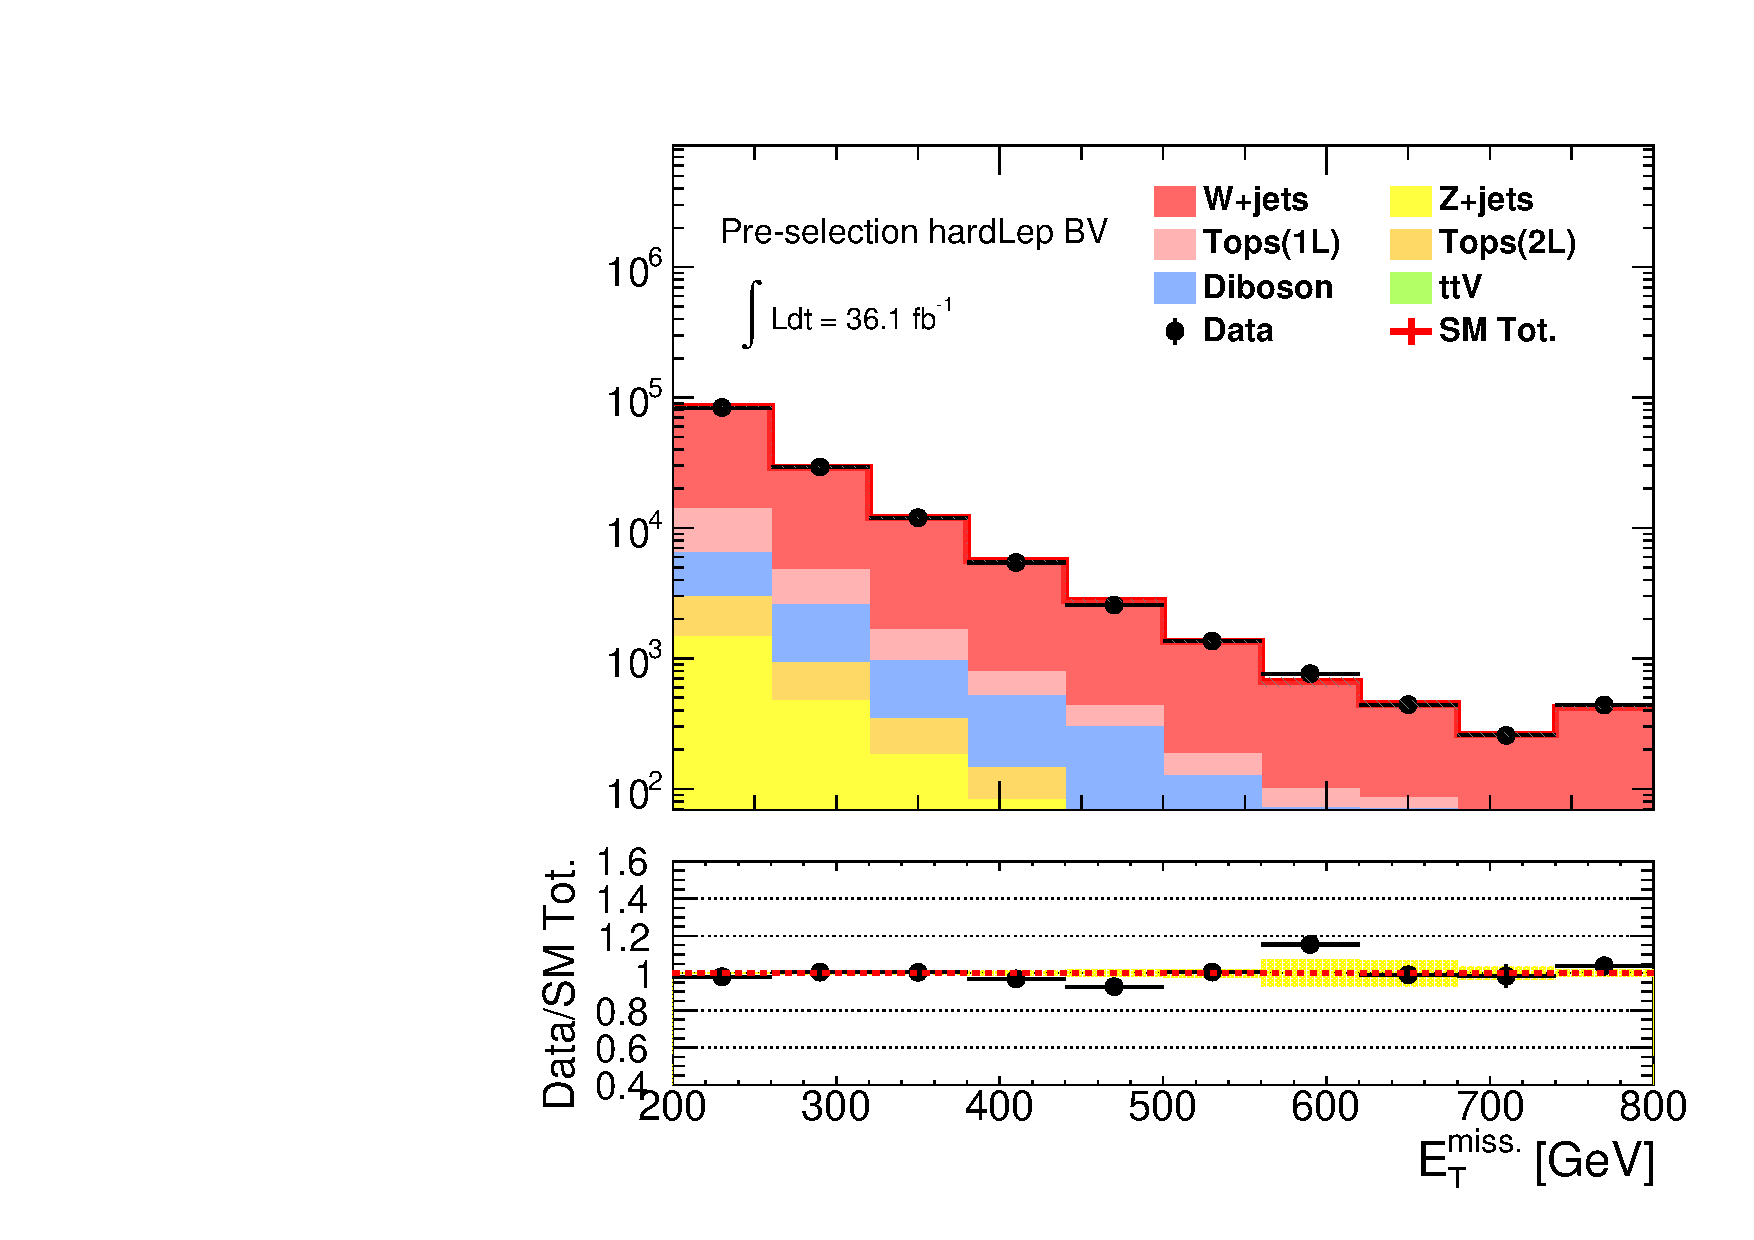
\includegraphics[width=0.48\textwidth]{figures/BGestimation/DataMCComparison/Preselection_hardLepBV/met__Preselection_hardLepBV__rwgt_nJ007_ttPt007.pdf}}
    \subfigure[]{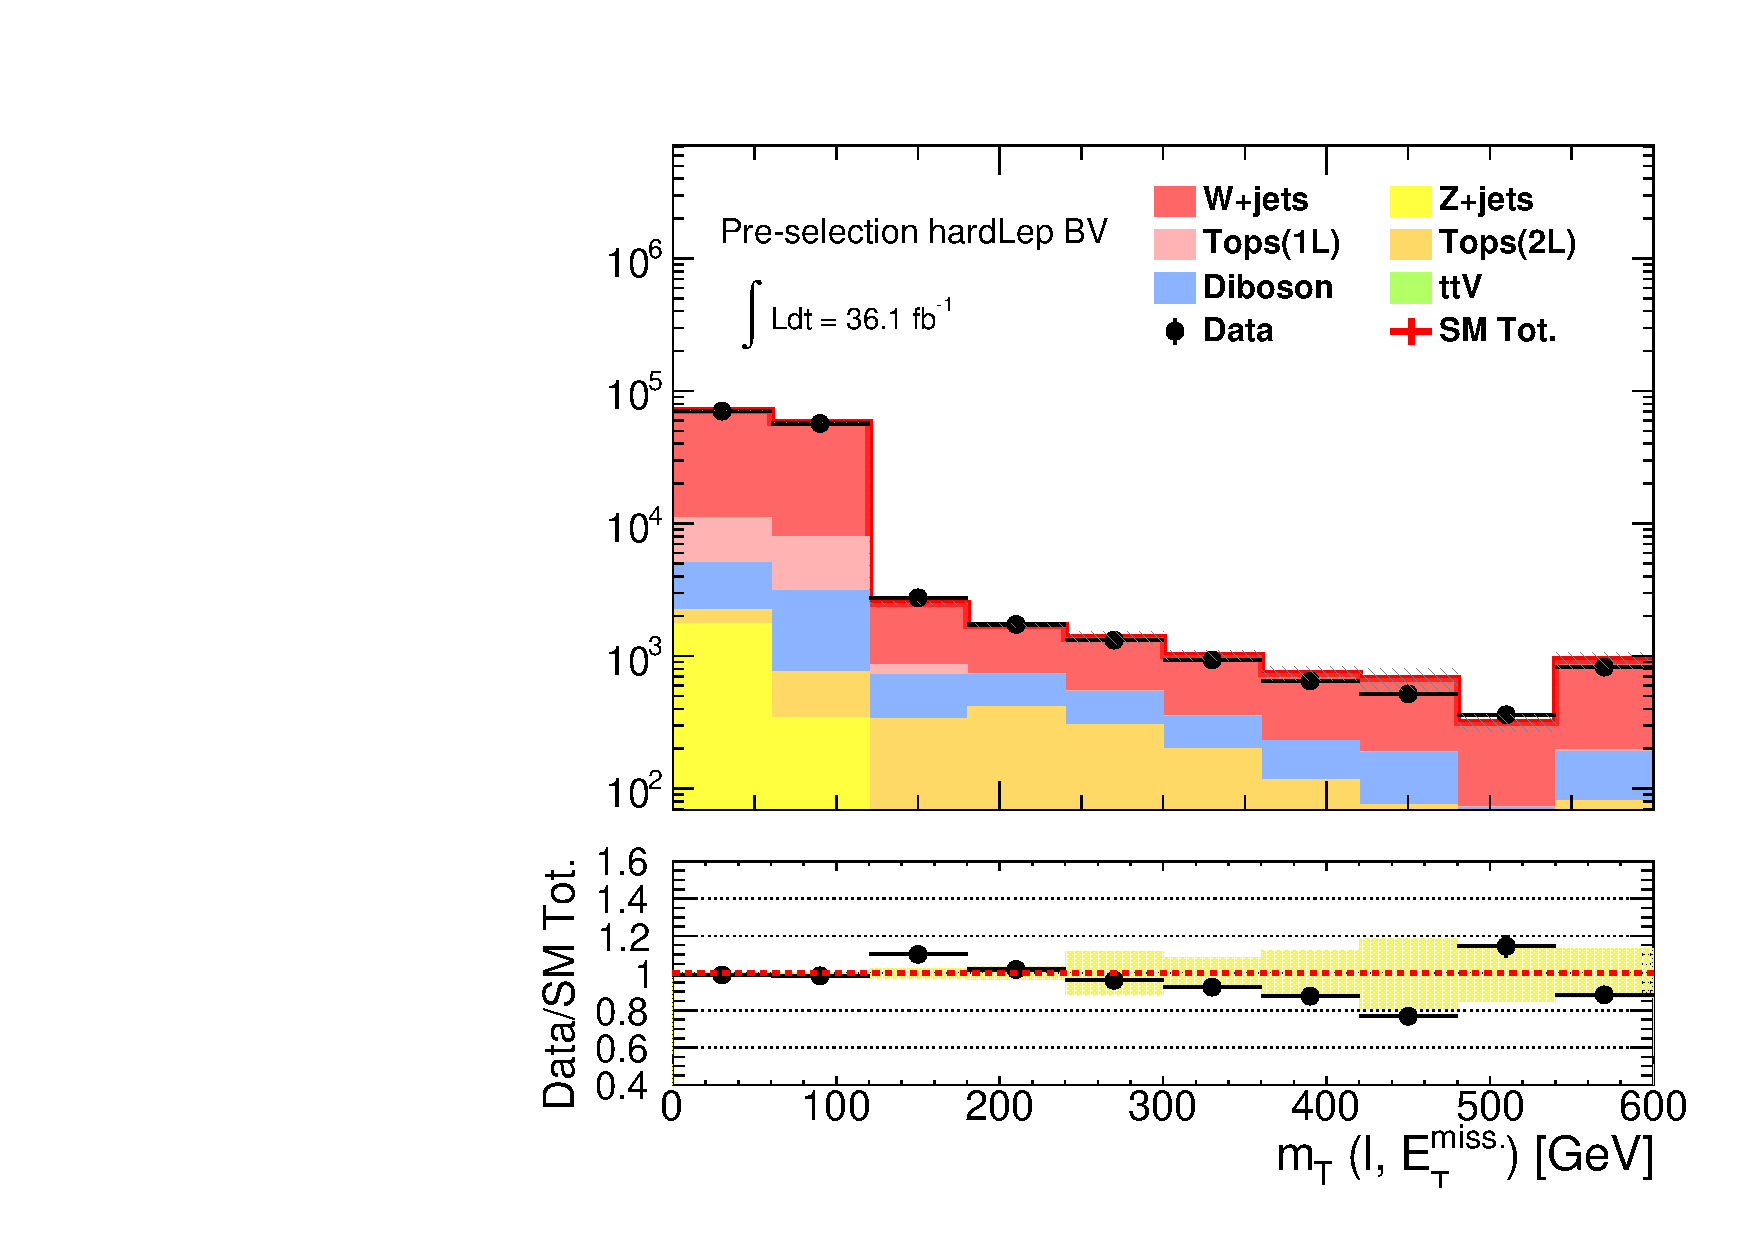
\includegraphics[width=0.48\textwidth]{figures/BGestimation/DataMCComparison/Preselection_hardLepBV/mt__Preselection_hardLepBV__rwgt_nJ007_ttPt007.pdf}}
    \subfigure[]{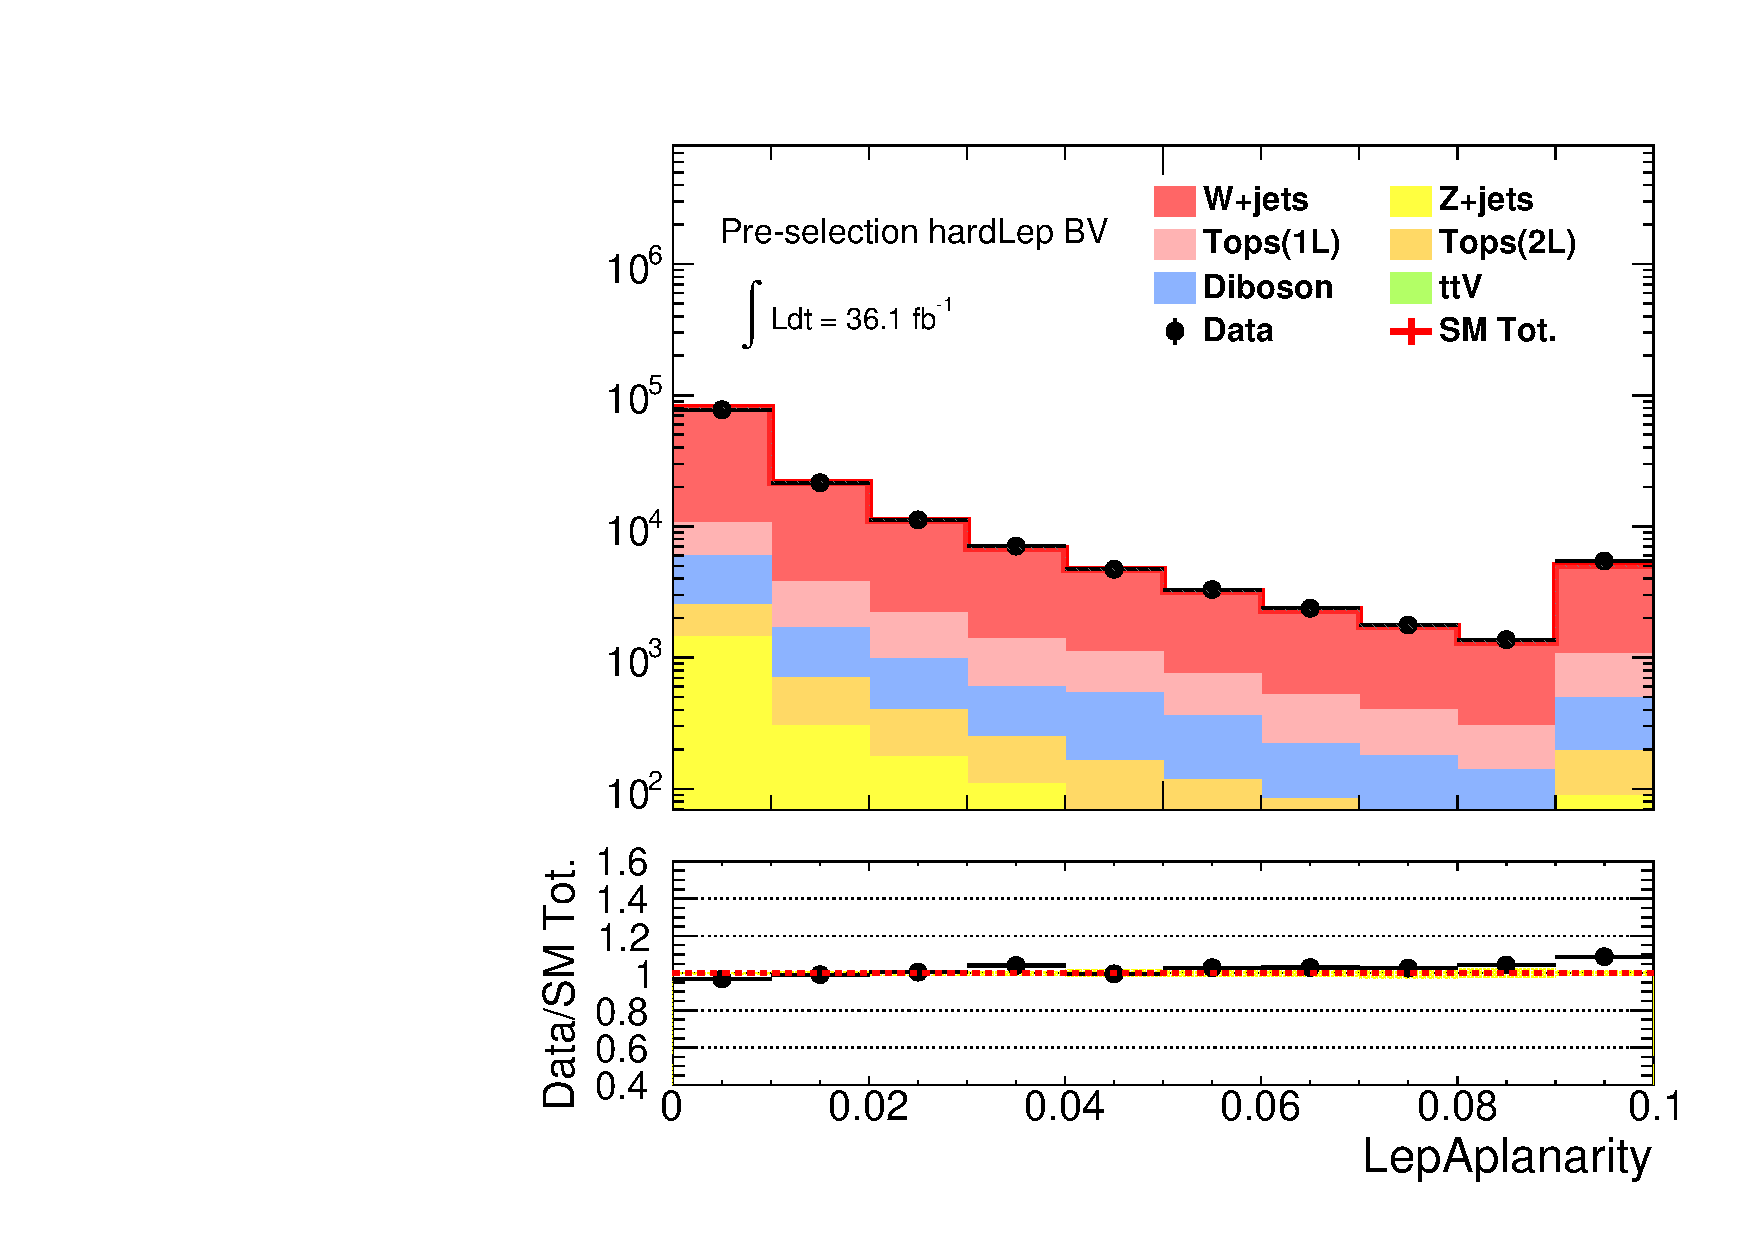
\includegraphics[width=0.48\textwidth]{figures/BGestimation/DataMCComparison/Preselection_hardLepBV/LepAplanarity__Preselection_hardLepBV__rwgt_nJ007_ttPt007.pdf}}
    \caption{ Kinematical distribution of (a) leading-lepton pt (b) $\met$  (c) $\mt$  (d) $\apl$ in the \textbf{hard lepton b-vetoed} pre-selection region, with the reweighting $w = 1 - 0.1 \times (\nJetNoGev-2)$ (Eq.(\ref{eq::BGestimation::rwgt_nJ})) being applied for $\wjets$ MC.  \label{fig::BGestimation::DataMCPreselHardBV_rwgt2} }
\end{figure}


%%%%%%%%%%%%%%
\begin{figure}[h]
  \centering
    \subfigure[]{\includegraphics[width=0.48\textwidth]{figures/BGestimation/DataMCComparison/Preselection_softLepBV/nJet30__Preselection_softLepBV.pdf}}
    \subfigure[]{\includegraphics[width=0.48\textwidth]{figures/BGestimation/DataMCComparison/Preselection_softLepBV/jet1Pt__Preselection_softLepBV.pdf}}
    \subfigure[]{\includegraphics[width=0.48\textwidth]{figures/BGestimation/DataMCComparison/Preselection_softLepBV/averageJetPt__Preselection_softLepBV.pdf}}
    \subfigure[]{\includegraphics[width=0.48\textwidth]{figures/BGestimation/DataMCComparison/Preselection_softLepBV/meffInc30__Preselection_softLepBV.pdf}}
    \caption{ Kinematical distribution of (a) Jet multiplicity ($p_T>30\gev$) (b) leading-jet pt  (c) average jet pt ($p_T>30\gev$)  (d) $\meffInc$ in the soft lepton b-vetoed pre-selection region.  \label{fig::BGestimation::DataMCPreselSoftBV1} }
\end{figure}

\begin{figure}[h]
  \centering
    \subfigure[]{\includegraphics[width=0.48\textwidth]{figures/BGestimation/DataMCComparison/Preselection_softLepBV/lep1Pt__Preselection_softLepBV.pdf}}
    \subfigure[]{\includegraphics[width=0.48\textwidth]{figures/BGestimation/DataMCComparison/Preselection_softLepBV/met__Preselection_softLepBV.pdf}}
    \subfigure[]{\includegraphics[width=0.48\textwidth]{figures/BGestimation/DataMCComparison/Preselection_softLepBV/mt__Preselection_softLepBV.pdf}}
    \subfigure[]{\includegraphics[width=0.48\textwidth]{figures/BGestimation/DataMCComparison/Preselection_softLepBV/LepAplanarity__Preselection_softLepBV.pdf}}
    \caption{ Kinematical distribution of (a) leading-lepton pt (b) $\met$  (c) $\mt$  (d) $\apl$ in the soft lepton b-vetoed pre-selection region.  \label{fig::BGestimation::DataMCPreselSoftBV2} }
\end{figure}

\clearpage
%%%%%%%%%%%%%


%%%%%%%%%%% VRZb
%\begin{figure}[h]
%  \centering
%    \subfigure[]{\includegraphics[width=0.48\textwidth]{figures/BGestimation/VRZb/mll__VRZb_log.pdf}}
%    \subfigure[]{\includegraphics[width=0.48\textwidth]{figures/BGestimation/VRZb/mll__VRZb__Zb130_log.pdf}}
%    \caption{ .  \label{fig::BGestimation::VRZb} }
%\end{figure}


%%%%%%%%%%%%%%%%%%%%%%%%%%%%%%%%%%%%%%%
\paragraph{Tops}
Figurere \ref{fig::BGestimation::DataMCPreselHardBV1} - \ref{fig::BGestimation::DataMCPreselHardBV2} are the kinematic distributions in the pre-selection region \textbf{1LBT hardLep} dominated by $\ttbar$.
It is seen that MC is overshooting the data with increasing transverse momenta of outgoing particles such as jets, lepton and MET. \\

In particular, the mis-modeling in $\meffInc$ distribution is significant. This is concerning given that the signal regions are designed to exploit its shape thereforewWe first try to understand the mis-modeling in $\meffInc$. The leading source of the mis-modeling is suspected to be in the description of ISR or FSR radiation. This is because hard jets ($\pt>200 \gev$) become more often non-$\ttbar$ origin in the tail of $\meffInc$, as demonstrated by Figurere \ref{fig::BGestimation::ISRFrac_ttbar}, although $\ttbar$ does have 2-4 jets in its tree-level decay. \\
This is in fact also supported by a series of MC reweighting studies shown in Figurere \ref{fig::BGestimation::slope_rwgt}  where linear reweighting in various top kinematic variables is attempted to correct the the slope of data/MC in $\meffInc$. It turns that $p_{T}(\ttbar)$ is the variable most sensitive to the mis-modeling, while reweighting in other variables can only change the normalization but the slope. This strongly indicates that the primary problem is in the radiation recoiling the $\ttbar$ rather than in the internal kinematics of the $\ttbar$ system. \\

%Therefore modeling of higher-order QCD/EW effects is again suspected as the cause of mis-modeling. \\
%Many explainatory higher-order effects have been proposed to account for the discrepancy, such as QCD-NNLO \cite{ttbar_NNLOQCD} or EW radiative correction \cite{ttbar_NLOEW}. \\
% top reweighiting の歴史

%%%%%%%%
\fig[100]{BGestimation/ISRFrac/ISRFrac_vs_meff.pdf}
{Fraction of ISR and FSR jets in the 4 leading jets with the largest transverse momenta, defined by $N_{\mathrm{events}}$($i$-th jets in the pt range that do not match either jets from ttbar decay by $\Delta R<0.2$)/$N_{\mathrm{events}}$(all $i$-th jets in the pt range).}
{fig::BGestimation::ISRFrac_ttbar}
%%%%%%%%

\begin{figure}[h]
  \centering
    \subfigure[]{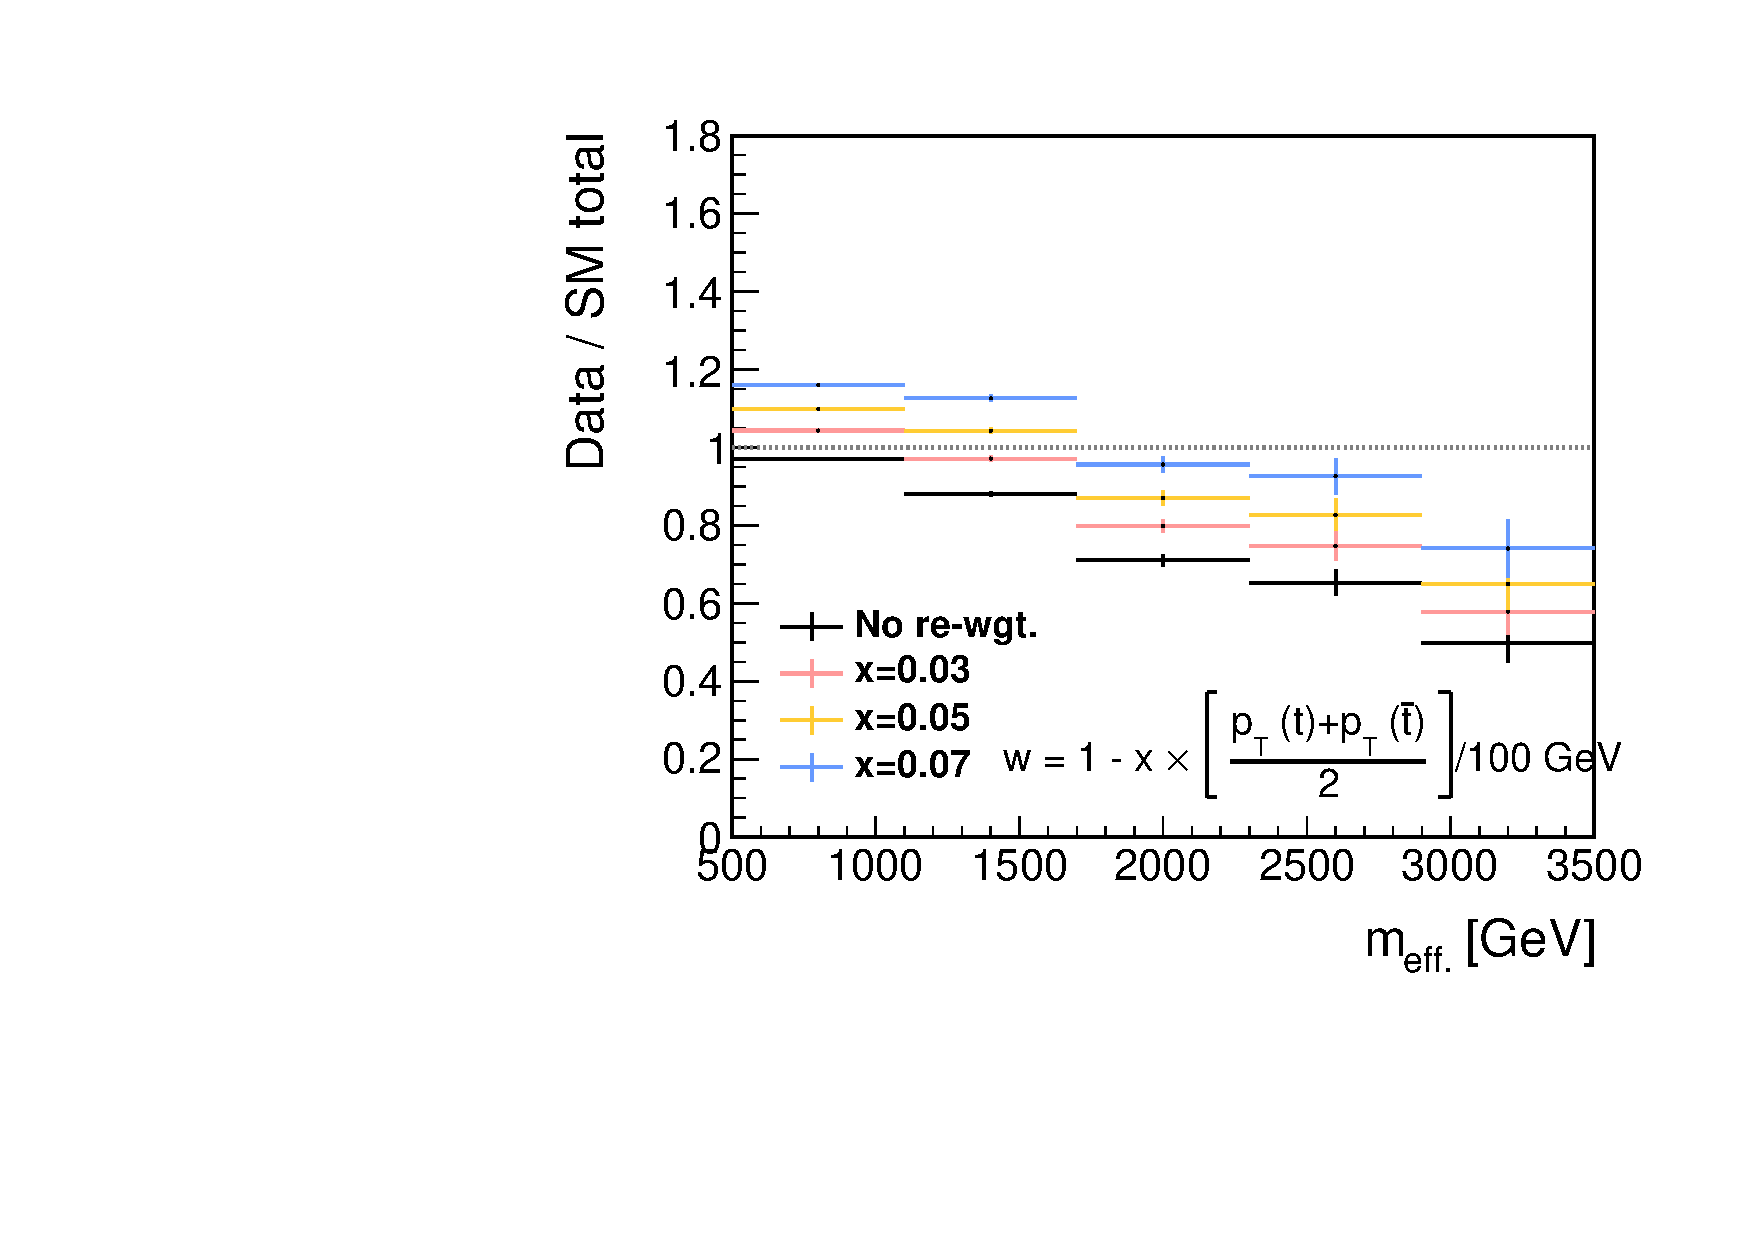
\includegraphics[width=0.48\textwidth]{figures/BGestimation/slope_rwgt/slopes_rwgt_topPt.pdf}}
    \subfigure[]{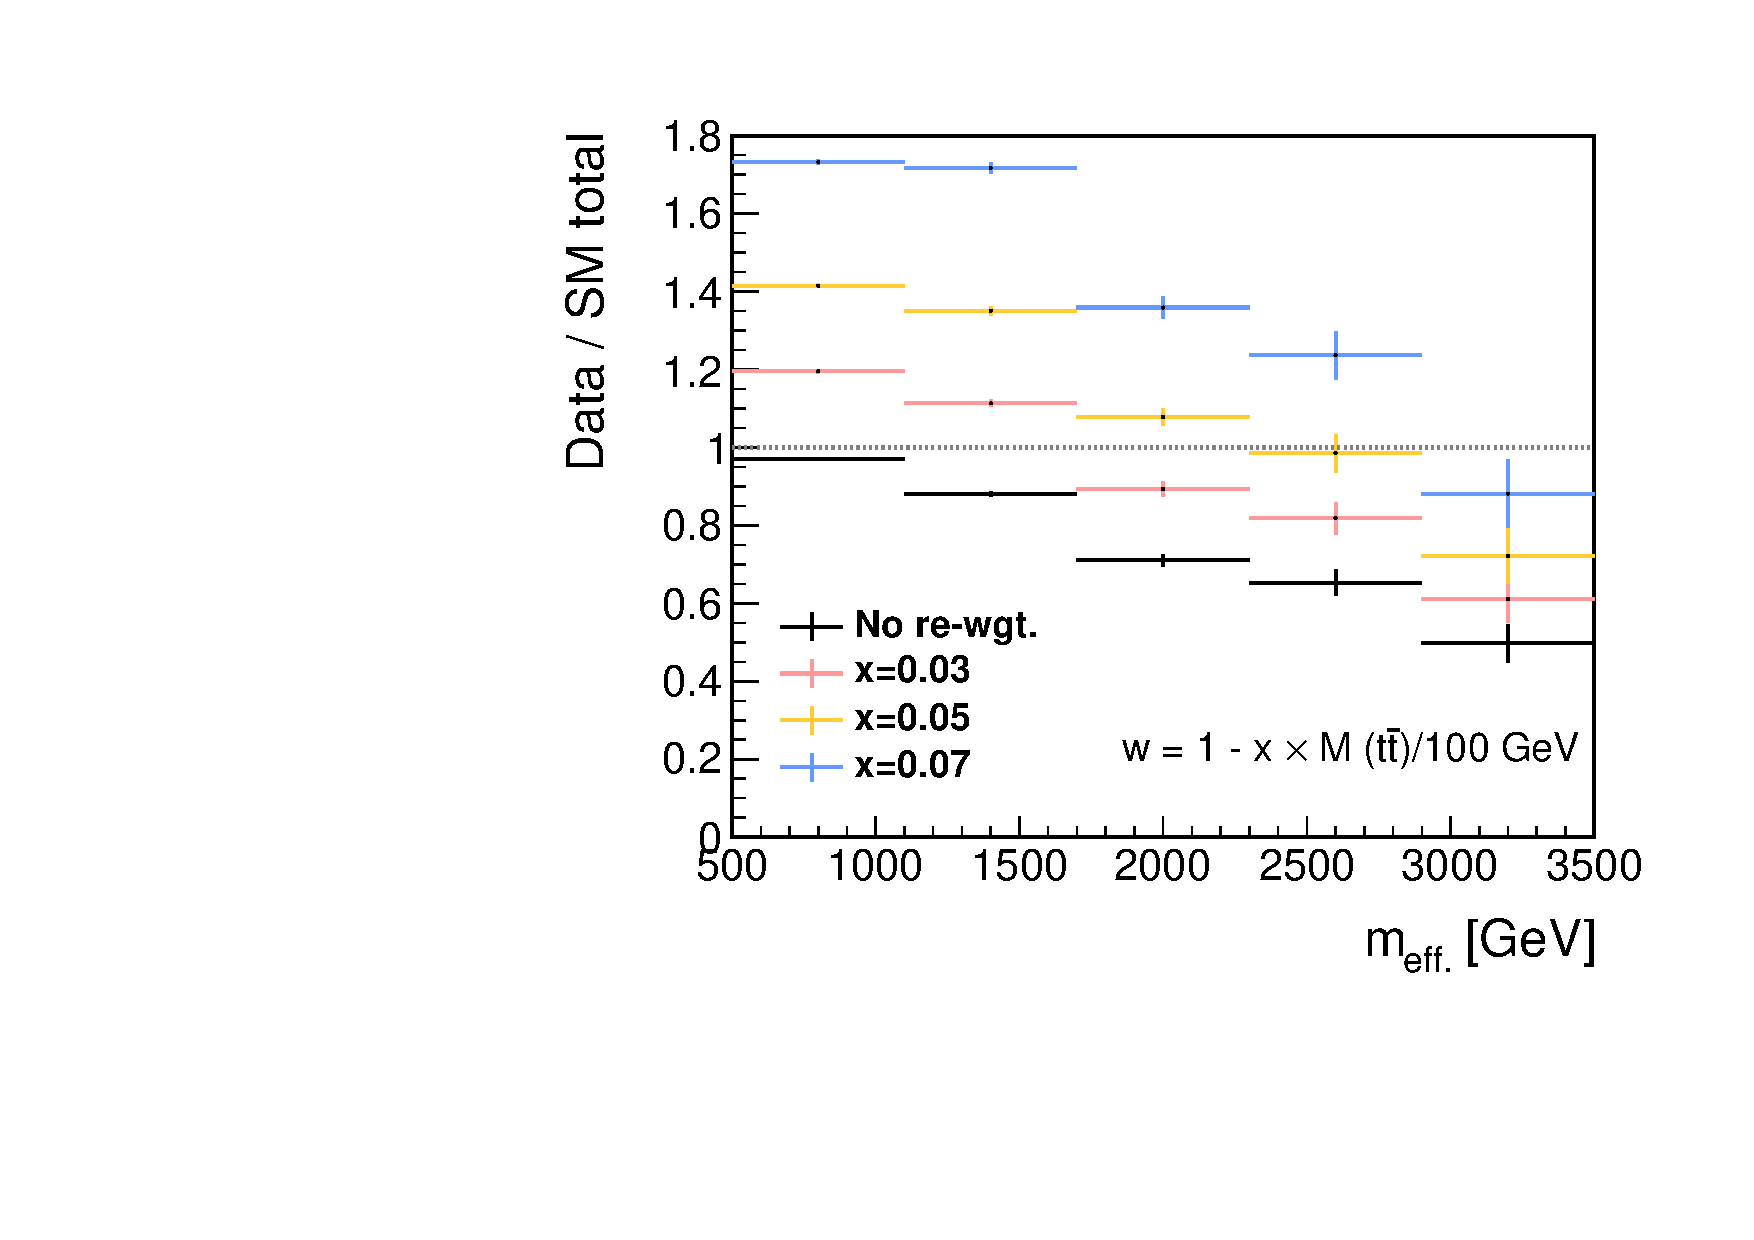
\includegraphics[width=0.48\textwidth]{figures/BGestimation/slope_rwgt/slopes_rwgt_ttM.pdf}}
    \subfigure[]{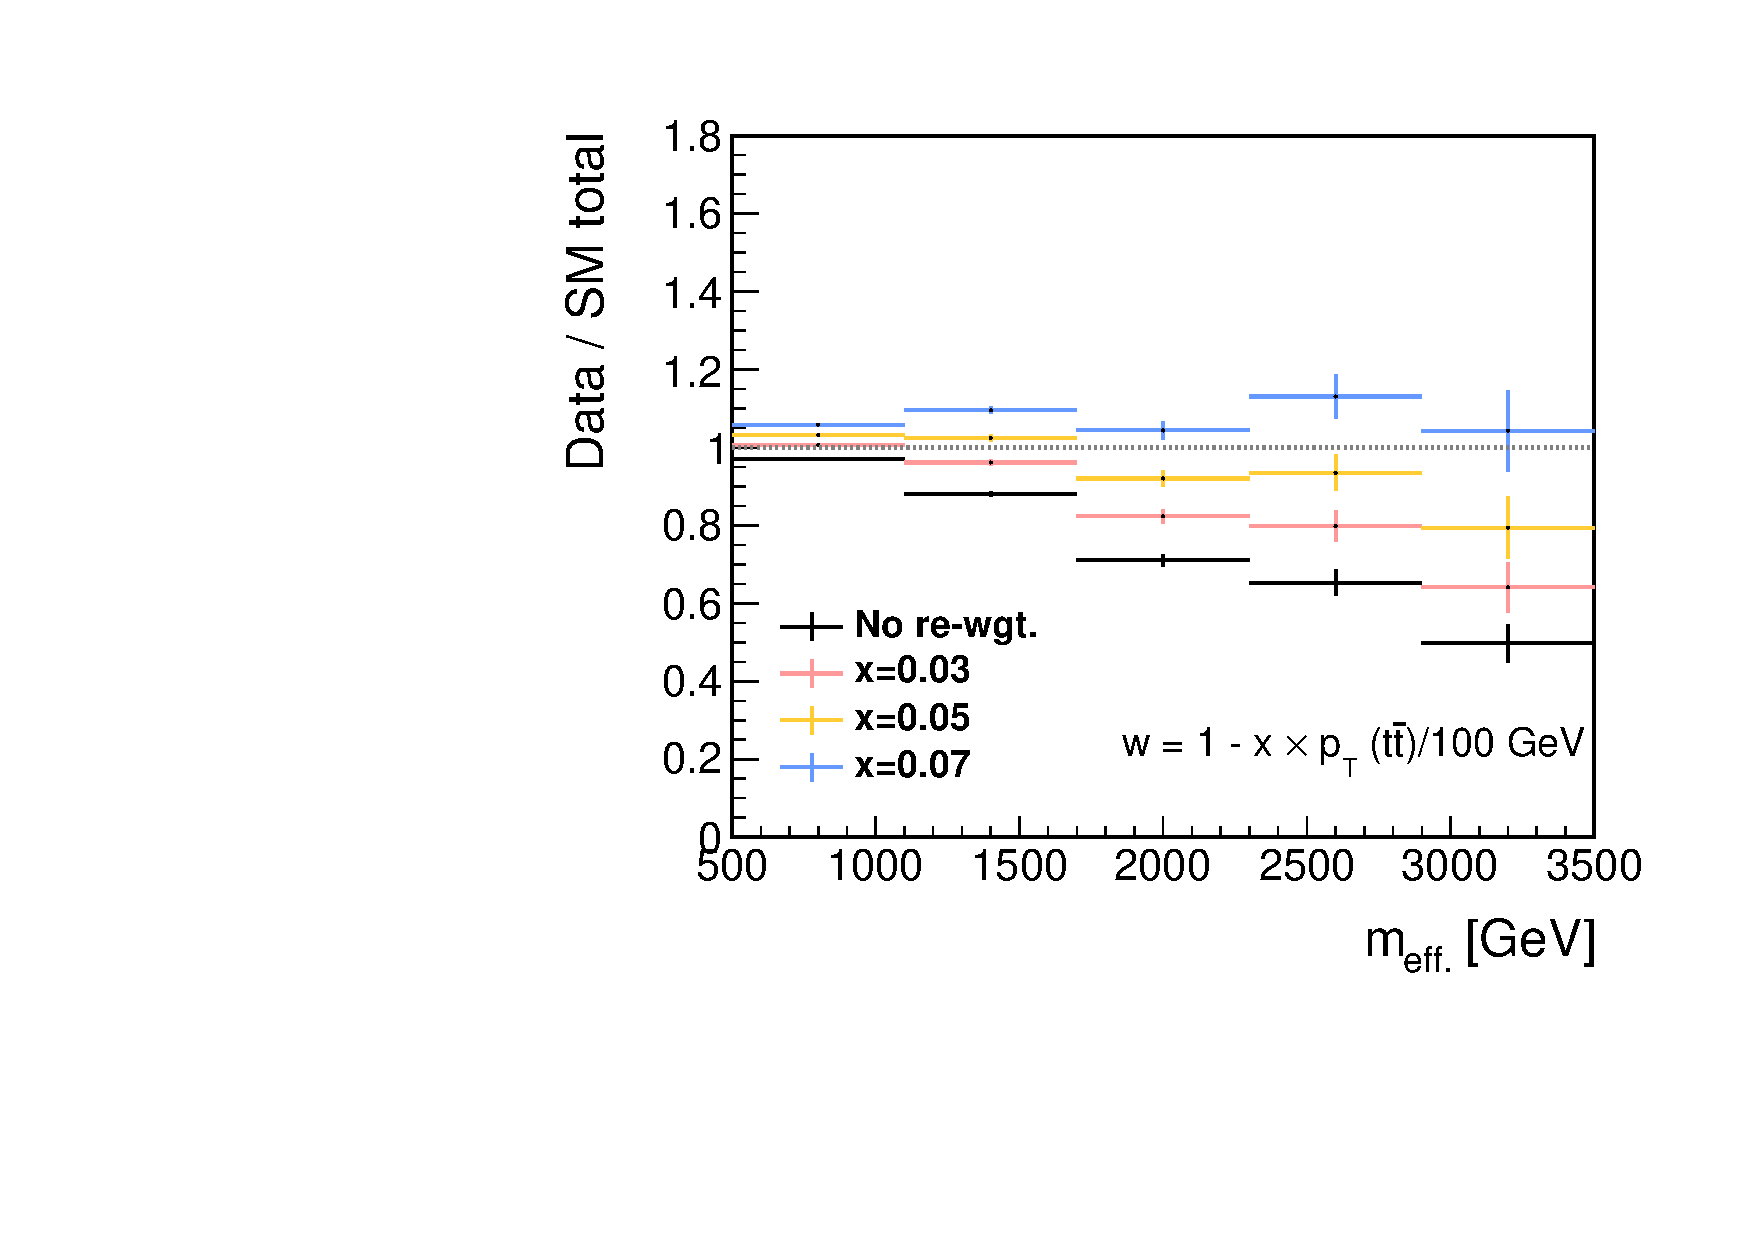
\includegraphics[width=0.48\textwidth]{figures/BGestimation/slope_rwgt/slopes_rwgt_ttPt.pdf}}
    \caption{ Response of data/MC in $\meffInc$ by reweighting $\ttbar$ events in terms of (a) average top transverse momentum
 ($(\pt(t)+\pt(\bar{t}))/2$), (b) invariant mass of $\ttbar$ system ($m_{\ttbar}$) and (c) transverse momentum of $\ttbar$ system ($\pt(\ttbar)$). $\pt(\ttbar)$ is found to be sensitive to the slope of $\meffInc$ and improve the data/MC discrepancy, while the other are only capable of shifting the normalization. 
\label{fig::BGestimation::slope_rwgt} }
\end{figure}


\clearpage
The $p_T(\ttbar)$-based reweighting is found also capable of restoring the discrepancy in other distribution other than $\meffInc$. Applying the reweighting function optimum for correcting the $\meffInc$:
\begin{align}
w = 1.05 \times \left[ 1 - 0.061 \,\times p_T(\ttbar) \right] \label{eq::BGestimation::rwgt_ttPt},
\end{align}
good data-MC agreement is seen in overall spectra regarding to jets and MET as shown in Figurere \ref{fig::BGestimation::DataMCPreselHardBT_rwgt1} - \ref{fig::BGestimation::DataMCPreselHardBT_rwgt2}. \\

The mis-modleing in lepton transverse momentum distribution seems to have the other origin, seen as the residual discrepancy . \\
%This ends up a small discrepancy in $\mt$ as well, 
%This is thought to be related to the modeling of top polarization which is difficult when higher order diagrams are significantly involved. This \\


\clearpage
\begin{figure}[h]
  \centering
    \subfigure[]{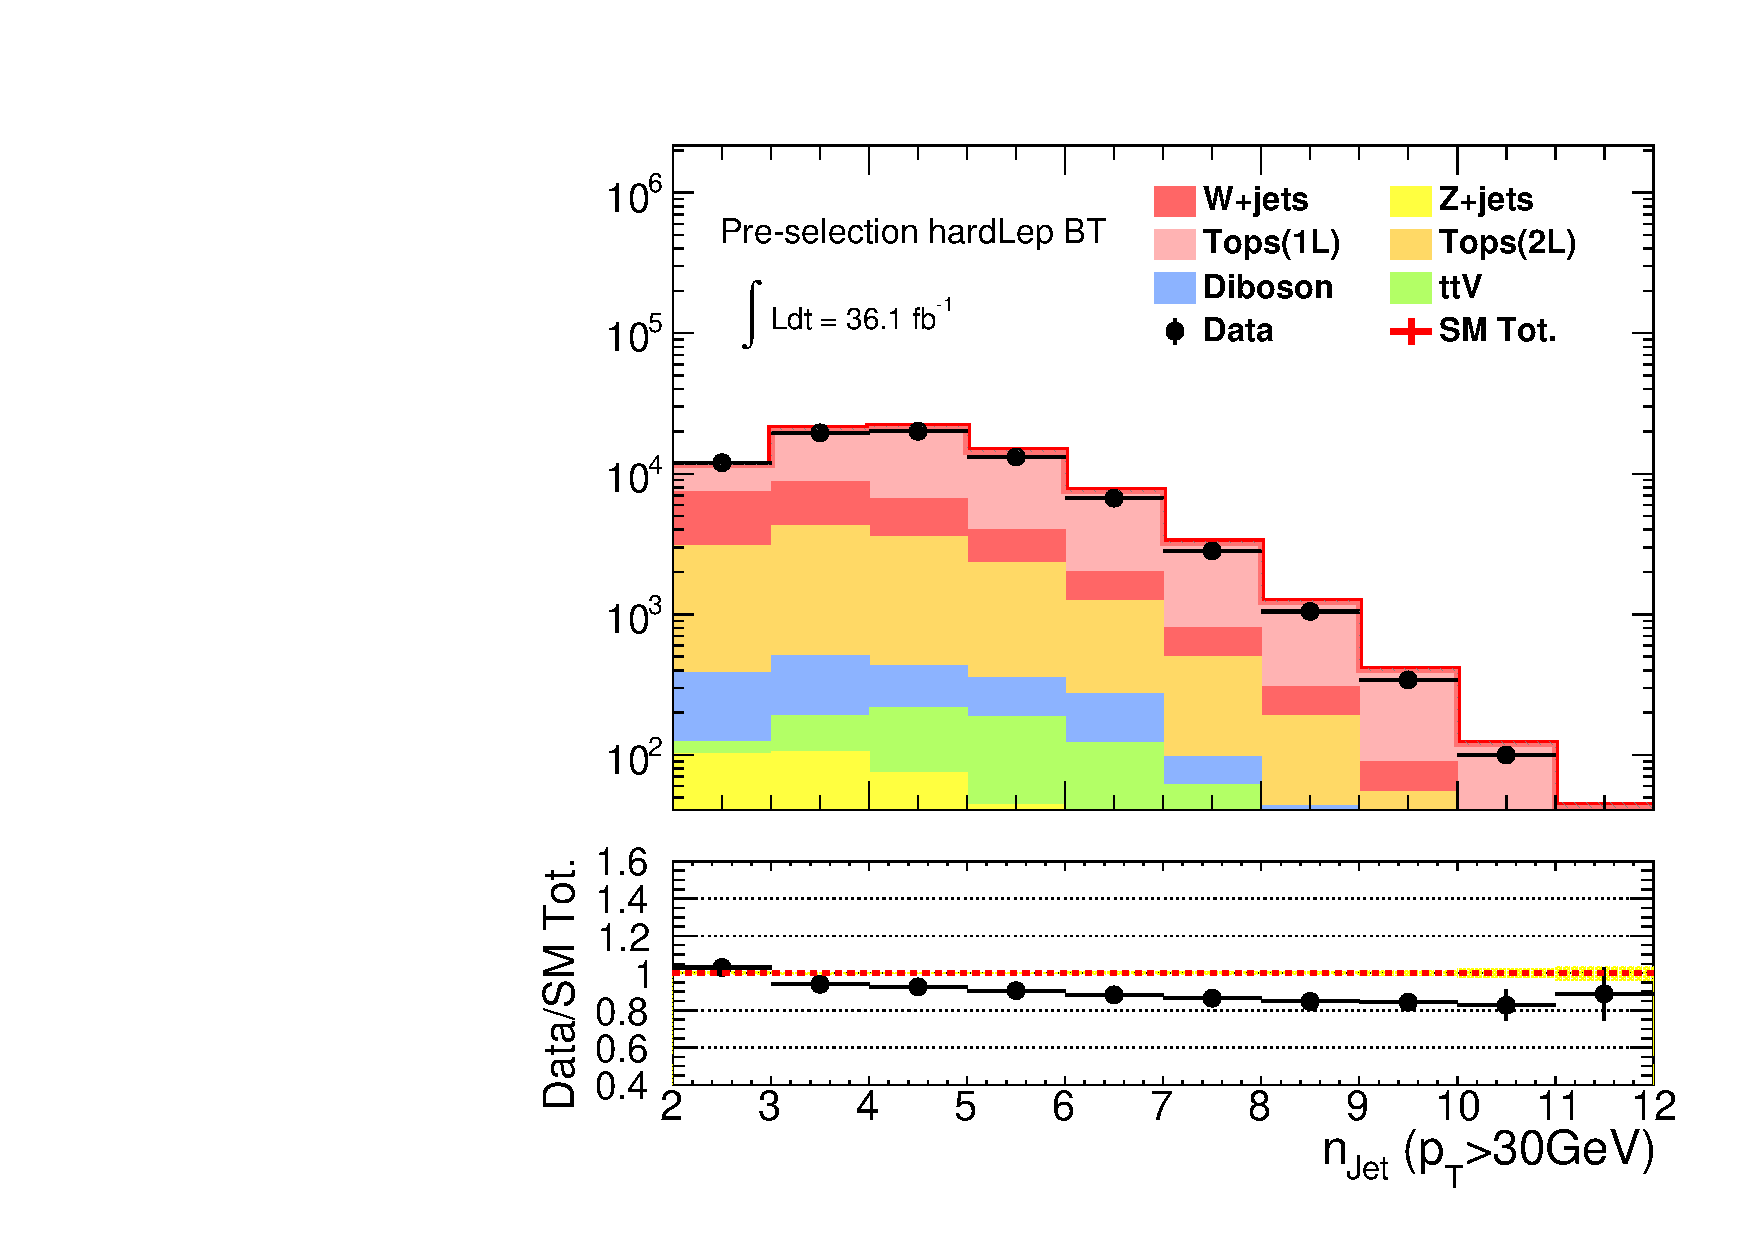
\includegraphics[width=0.48\textwidth]{figures/BGestimation/DataMCComparison/Preselection_hardLepBT/nJet30__Preselection_hardLepBT.pdf}}
    \subfigure[]{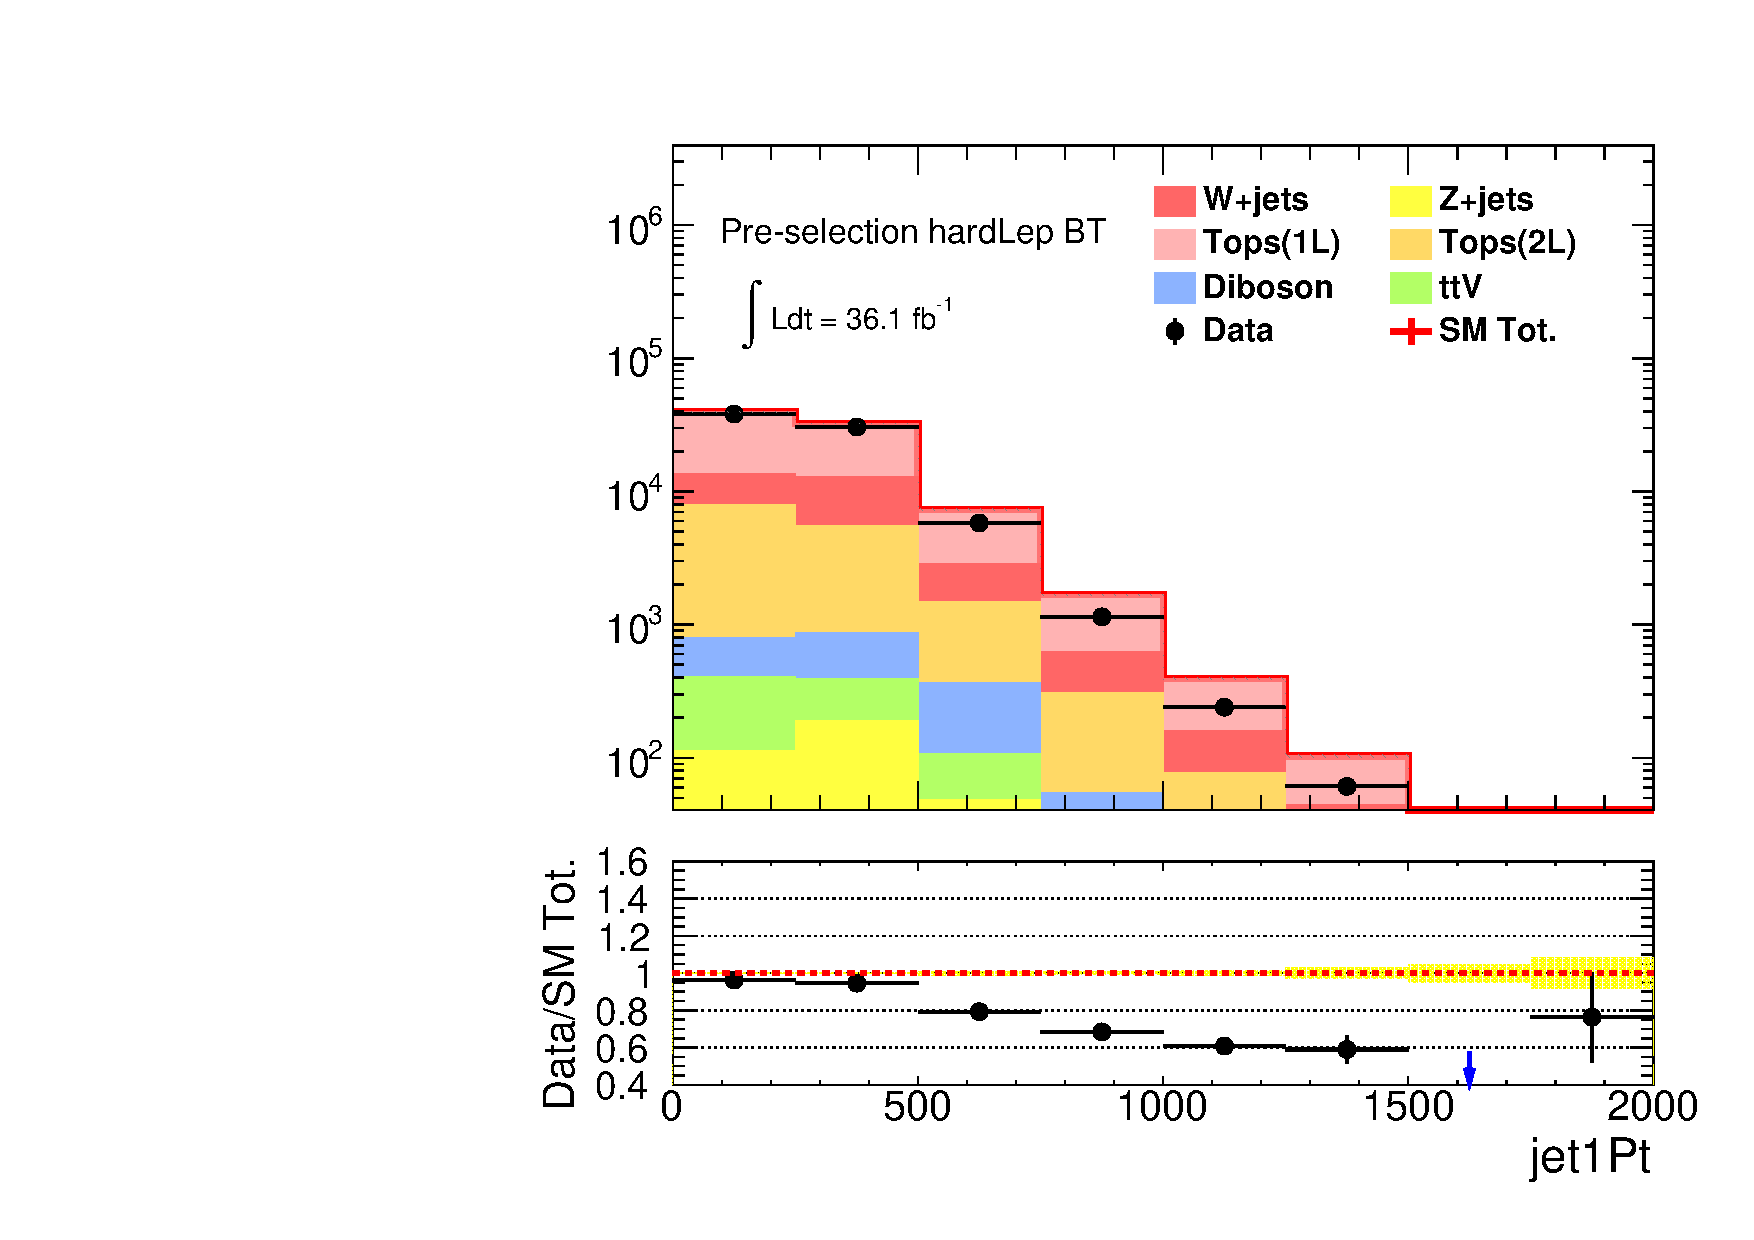
\includegraphics[width=0.48\textwidth]{figures/BGestimation/DataMCComparison/Preselection_hardLepBT/jet1Pt__Preselection_hardLepBT.pdf}}
    \subfigure[]{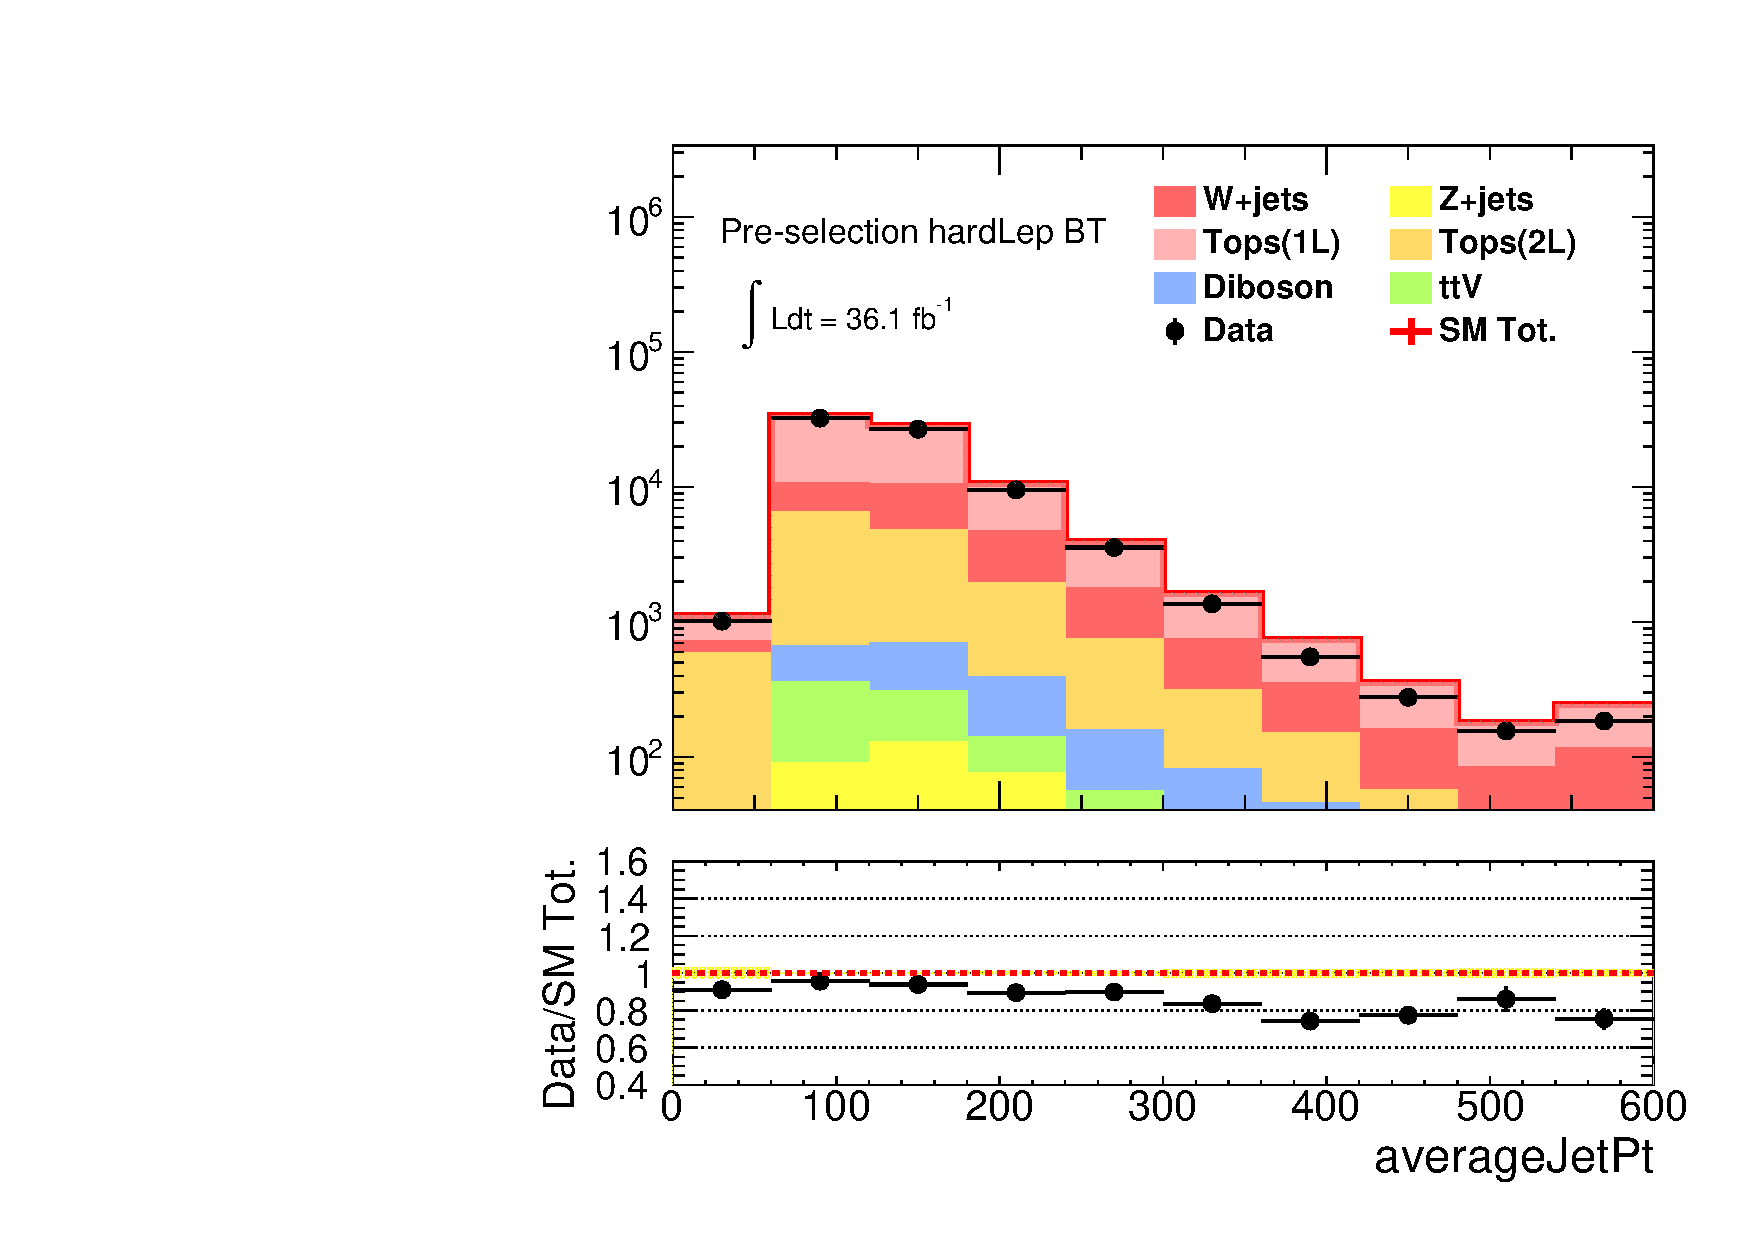
\includegraphics[width=0.48\textwidth]{figures/BGestimation/DataMCComparison/Preselection_hardLepBT/averageJetPt__Preselection_hardLepBT.pdf}}
    \subfigure[]{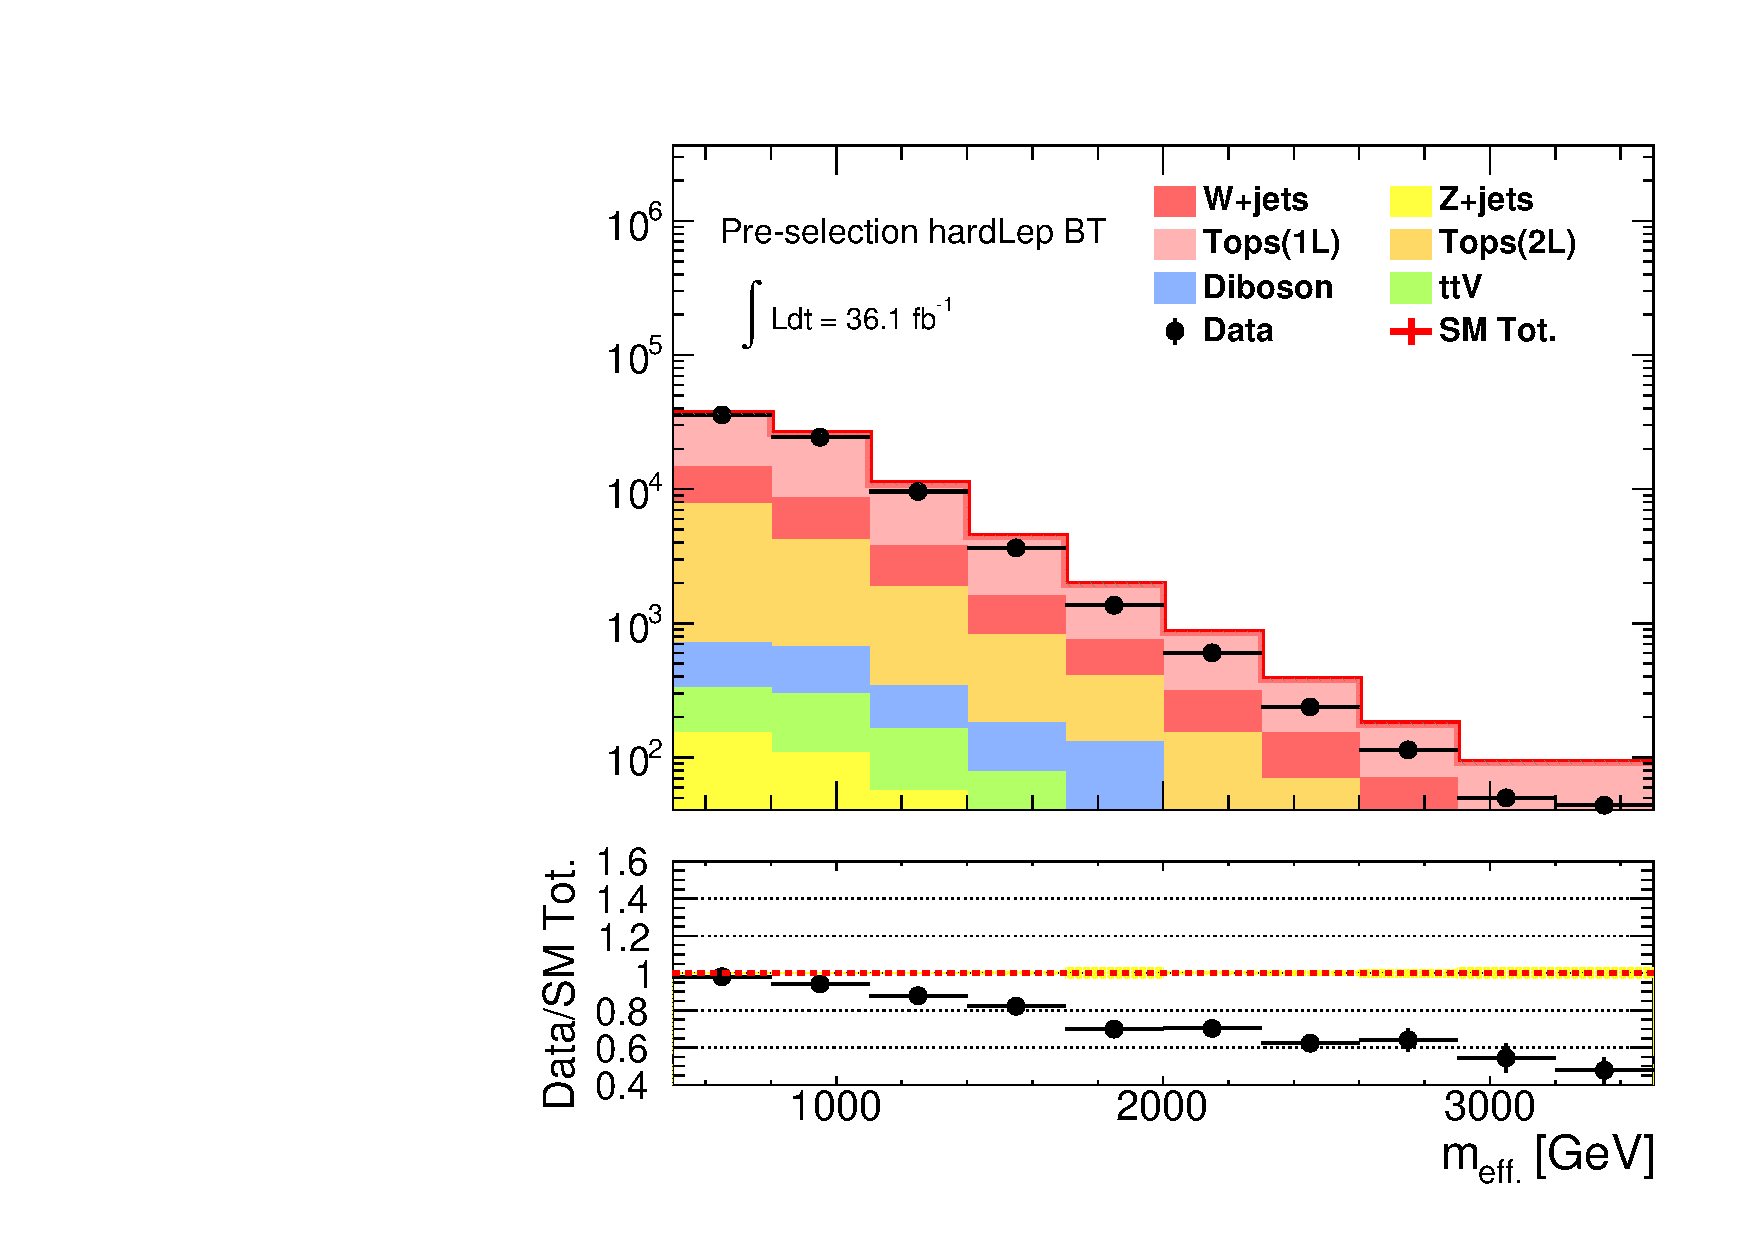
\includegraphics[width=0.48\textwidth]{figures/BGestimation/DataMCComparison/Preselection_hardLepBT/meffInc30__Preselection_hardLepBT.pdf}}
    \caption{ Kinematical distribution of (a) Jet multiplicity ($p_T>30\gev$) (b) leading-jet pt  (c) average jet pt ($p_T>30\gev$)  (d) $\meffInc$ in the hard lepton b-tagged pre-selection region.  \label{fig::BGestimation::DataMCPreselHardBT1} }
\end{figure}

\begin{figure}[h]
  \centering
    \subfigure[]{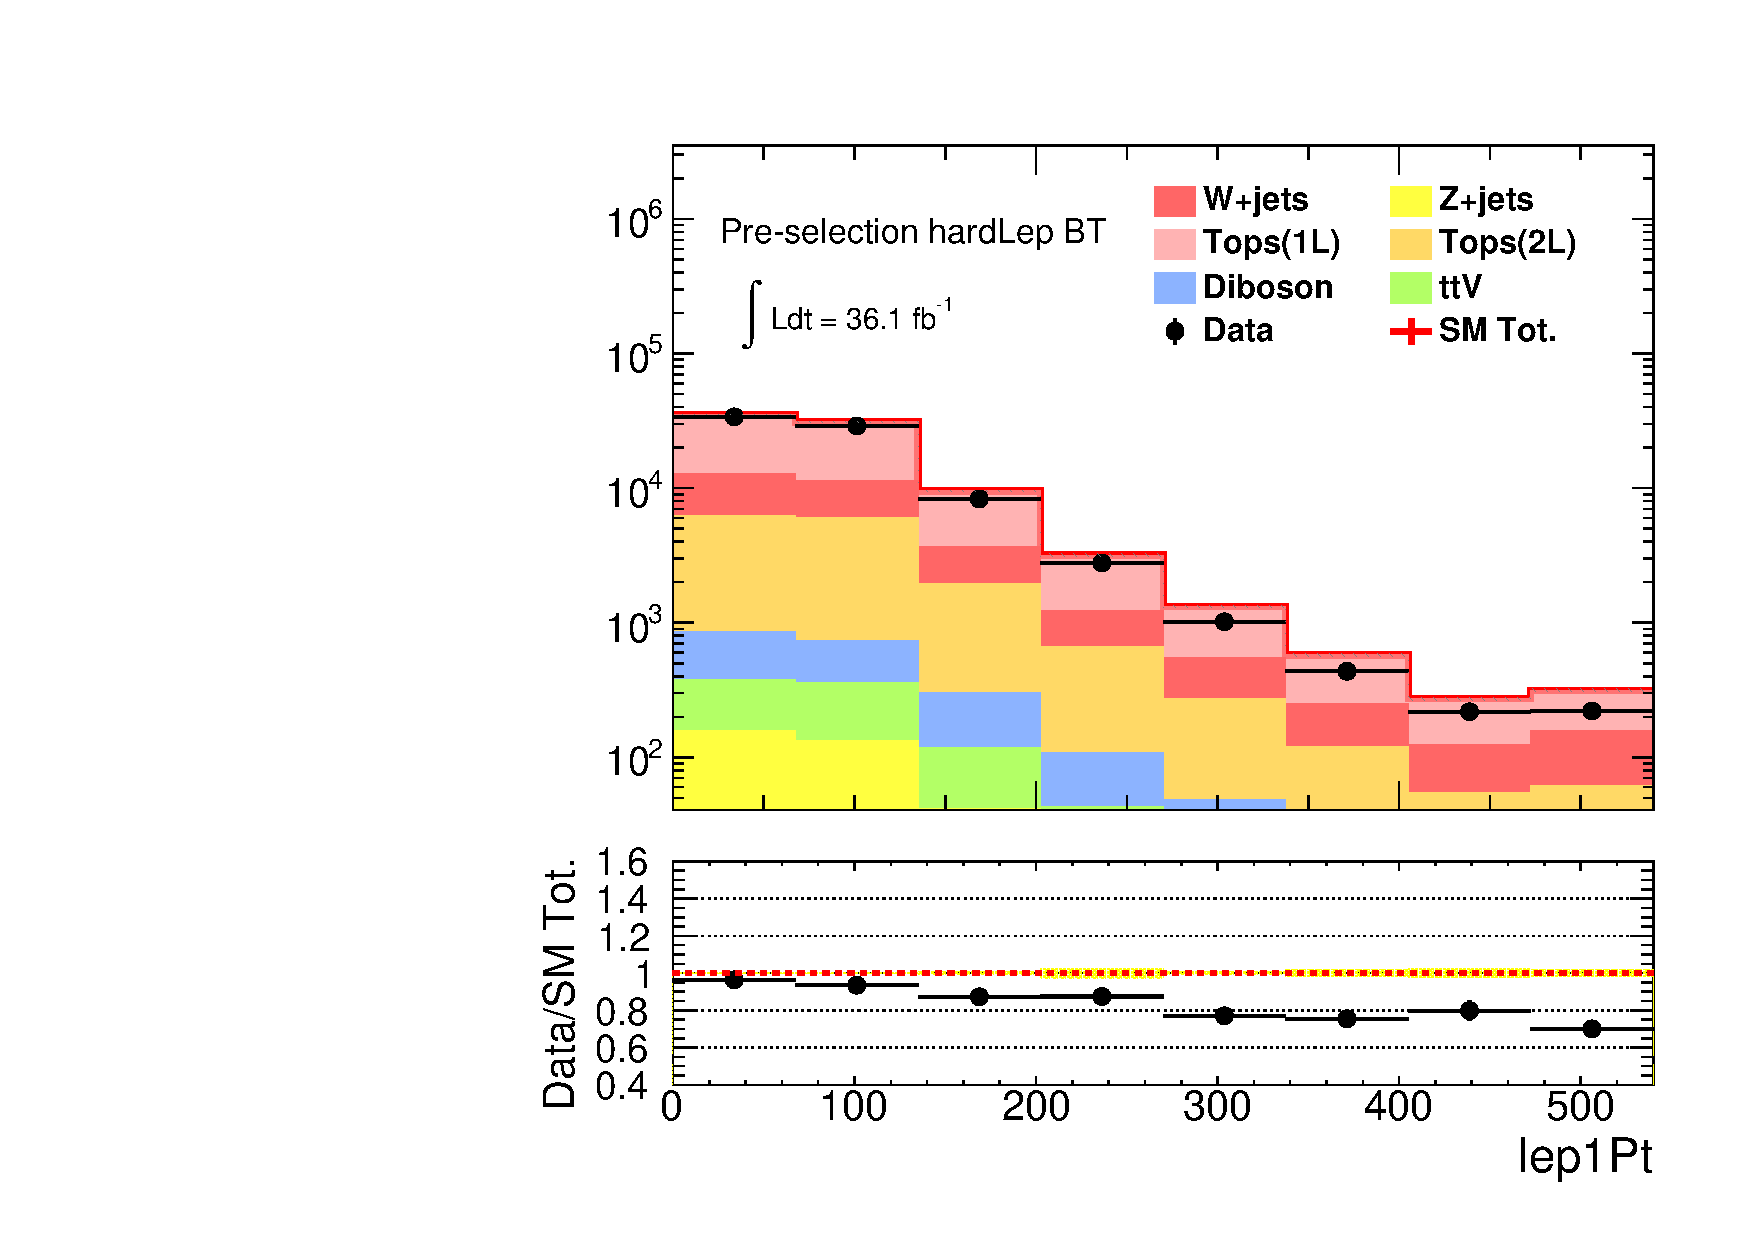
\includegraphics[width=0.48\textwidth]{figures/BGestimation/DataMCComparison/Preselection_hardLepBT/lep1Pt__Preselection_hardLepBT.pdf}}
    \subfigure[]{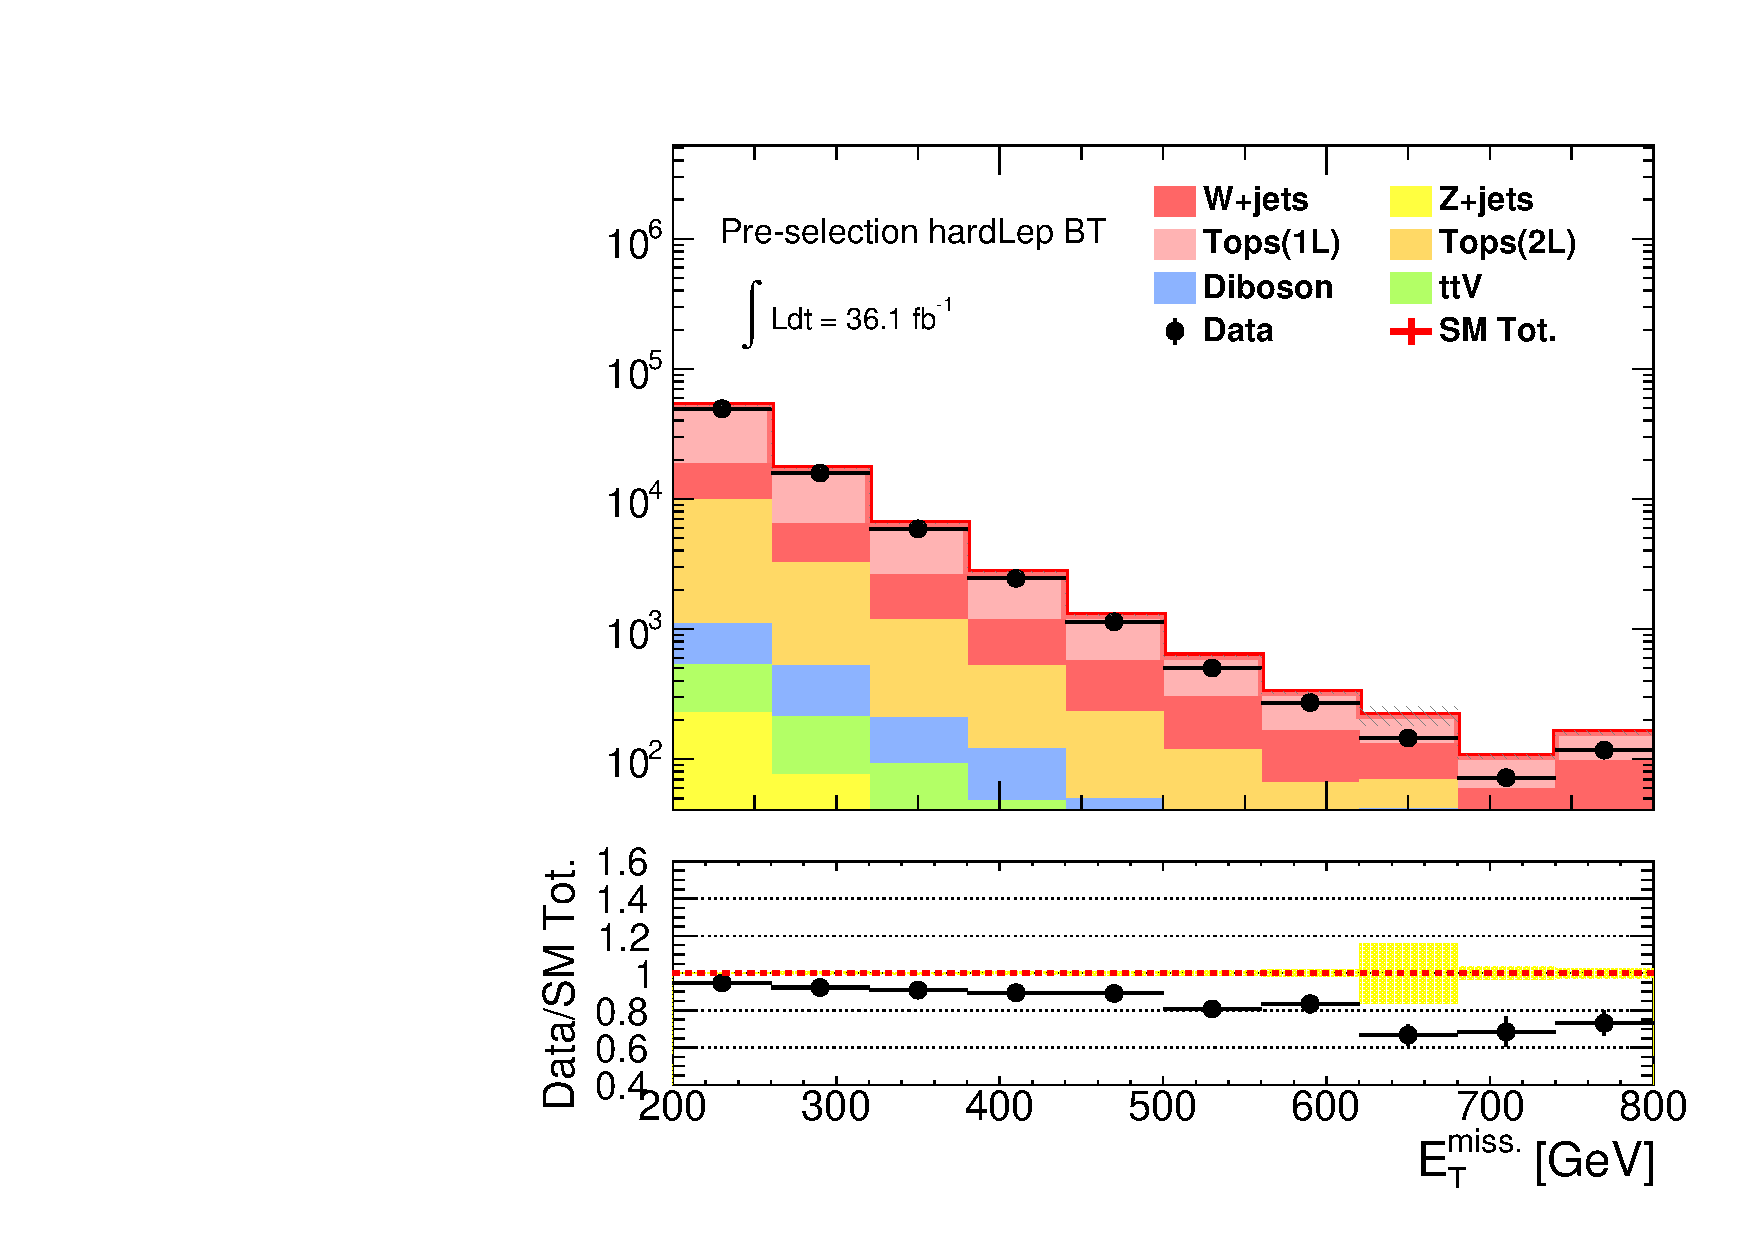
\includegraphics[width=0.48\textwidth]{figures/BGestimation/DataMCComparison/Preselection_hardLepBT/met__Preselection_hardLepBT.pdf}}
    \subfigure[]{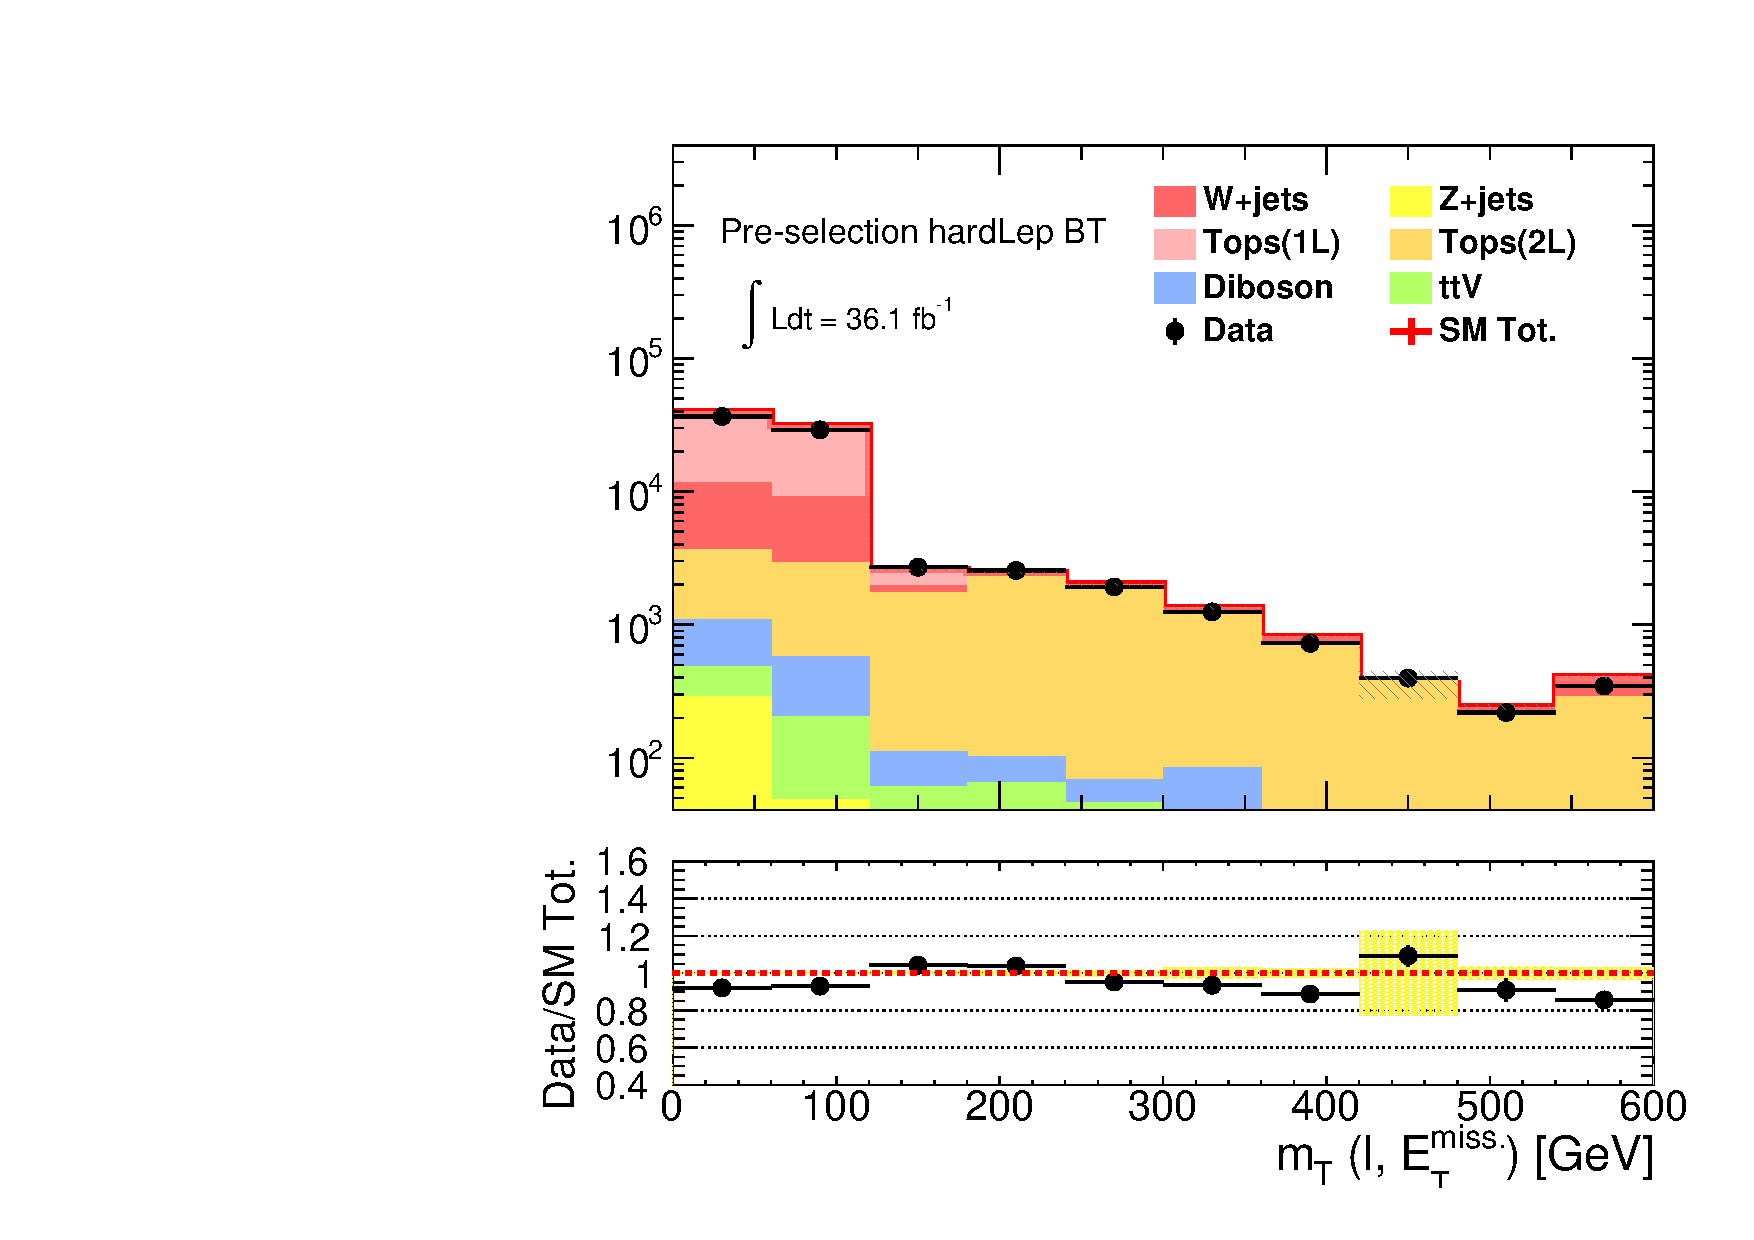
\includegraphics[width=0.48\textwidth]{figures/BGestimation/DataMCComparison/Preselection_hardLepBT/mt__Preselection_hardLepBT.pdf}}
    \subfigure[]{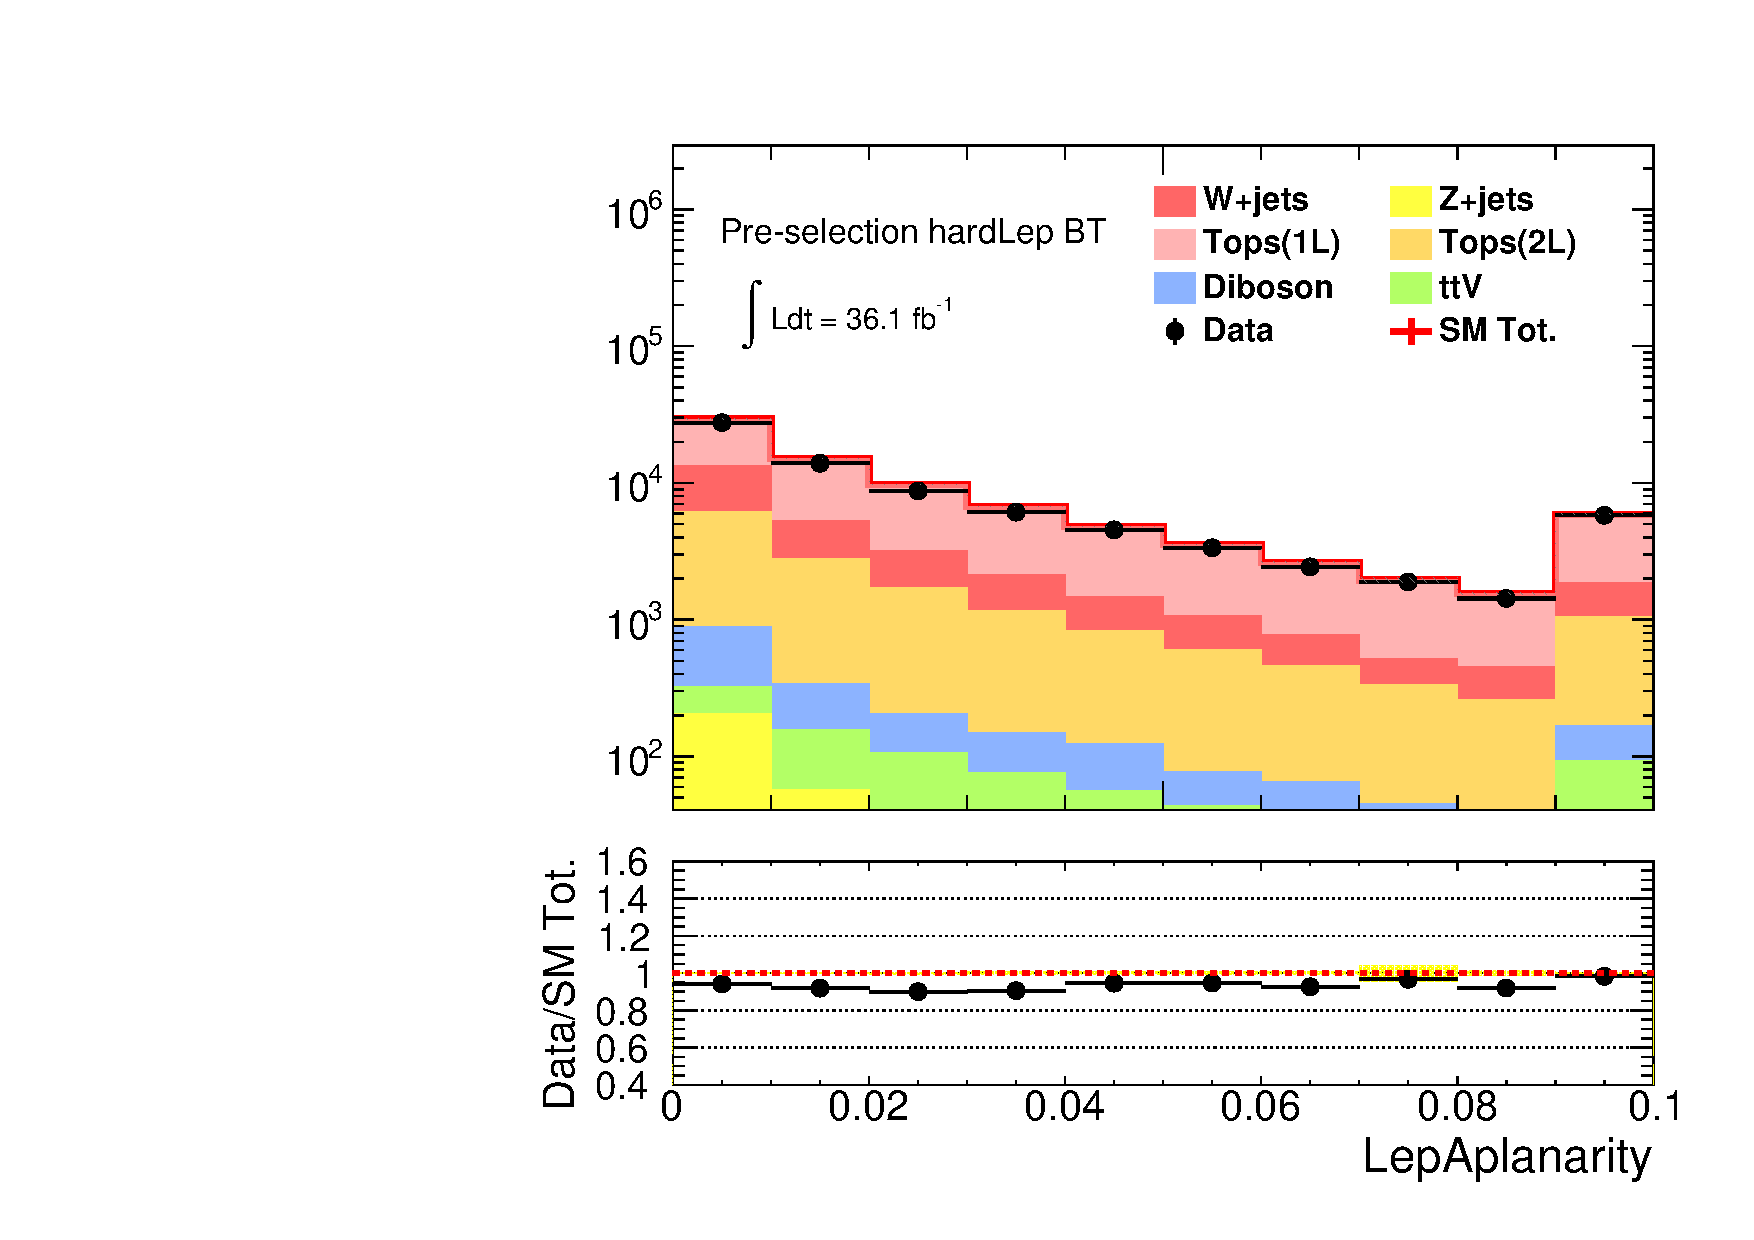
\includegraphics[width=0.48\textwidth]{figures/BGestimation/DataMCComparison/Preselection_hardLepBT/LepAplanarity__Preselection_hardLepBT.pdf}}
    \caption{ Kinematical distribution of (a) leading-lepton pt (b) $\met$  (c) $\mt$  (d) $\apl$ in the hard lepton b-tagged pre-selection region.  \label{fig::BGestimation::DataMCPreselHardBT2} }
\end{figure}
%%%%%%%%%%%%%

%%%%%%%%%%%%%
\begin{figure}[h]
  \centering
    \subfig{0.47}{figures/BGestimation/DataMCComparison/Preselection_hardLepBT/nJet30__Preselection_hardLepBT__rwgt_nJ007_ttPt007.pdf}{Jet multiplicity}
    \subfig{0.47}{figures/BGestimation/DataMCComparison/Preselection_hardLepBT/jet1Pt__Preselection_hardLepBT__rwgt_nJ007_ttPt007.pdf}{$\pt$ of the leading jet}
    \subfig{0.47}{figures/BGestimation/DataMCComparison/Preselection_hardLepBT/averageJetPt__Preselection_hardLepBT__rwgt_nJ007_ttPt007.pdf}{Average $\pt$ of jets with $\pt>30\gev$}
    \subfig{0.47}{figures/BGestimation/DataMCComparison/Preselection_hardLepBT/meffInc30__Preselection_hardLepBT__rwgt_nJ007_ttPt007.pdf}{$\meffInc (\meffDef)$}
    \caption{ Kinematical distribution of data (black dots) and MC (colored stack) in the \textbf{1LBT} pre-selection region, reweighting $w = 1.05 \times \left[ 1 - 0.061 \,\times p_T(\ttbar) \right]$ being applied for $\ttbar$ MC. 
 \label{fig::BGestimation::DataMCPreselHardBT_rwgt1} }
\end{figure}

\begin{figure}[h]
  \centering
    \subfig{0.48}{figures/BGestimation/DataMCComparison/Preselection_hardLepBT/lep1Pt__Preselection_hardLepBT__rwgt_nJ007_ttPt007.pdf}{Lepton's $\pt$}
    \subfig{0.48}{figures/BGestimation/DataMCComparison/Preselection_hardLepBT/met__Preselection_hardLepBT__rwgt_nJ007_ttPt007.pdf}{$\met$}
    \subfig{0.48}{figures/BGestimation/DataMCComparison/Preselection_hardLepBT/mt__Preselection_hardLepBT__rwgt_nJ007_ttPt007.pdf}{$\mt$}
    \subfig{0.48}{figures/BGestimation/DataMCComparison/Preselection_hardLepBT/LepAplanarity__Preselection_hardLepBT__rwgt_nJ007_ttPt007.pdf}{$\Apl$}
    \caption{ Kinematical distribution of data (black dots) and MC (colored stack) in the \textbf{1LBT} pre-selection region, with the reweighting $w = 1.05 \times \left[ 1 - 0.061 \,\times p_T(\ttbar) \right]$ being applied for $\ttbar$ MC.  \label{fig::BGestimation::DataMCPreselHardBT_rwgt2} }
\end{figure}


%%%%%%%%%%%%%%
\begin{figure}[h]
  \centering
    \subfigure[]{\includegraphics[width=0.48\textwidth]{figures/BGestimation/DataMCComparison/Preselection_softLepBT/nJet30__Preselection_softLepBT.pdf}}
    \subfigure[]{\includegraphics[width=0.48\textwidth]{figures/BGestimation/DataMCComparison/Preselection_softLepBT/jet1Pt__Preselection_softLepBT.pdf}}
    \subfigure[]{\includegraphics[width=0.48\textwidth]{figures/BGestimation/DataMCComparison/Preselection_softLepBT/averageJetPt__Preselection_softLepBT.pdf}}
    \subfigure[]{\includegraphics[width=0.48\textwidth]{figures/BGestimation/DataMCComparison/Preselection_softLepBT/meffInc30__Preselection_softLepBT.pdf}}
    \caption{ Kinematical distribution of (a) Jet multiplicity ($p_T>30\gev$) (b) leading-jet pt  (c) average jet pt ($p_T>30\gev$)  (d) $\meffInc$ in the soft lepton b-tagged pre-selection region.  \label{fig::BGestimation::DataMCPreselSoftBT1} }
\end{figure}

\begin{figure}[h]
  \centering
    \subfigure[]{\includegraphics[width=0.48\textwidth]{figures/BGestimation/DataMCComparison/Preselection_softLepBT/lep1Pt__Preselection_softLepBT.pdf}}
    \subfigure[]{\includegraphics[width=0.48\textwidth]{figures/BGestimation/DataMCComparison/Preselection_softLepBT/met__Preselection_softLepBT.pdf}}
    \subfigure[]{\includegraphics[width=0.48\textwidth]{figures/BGestimation/DataMCComparison/Preselection_softLepBT/mt__Preselection_softLepBT.pdf}}
    \subfigure[]{\includegraphics[width=0.48\textwidth]{figures/BGestimation/DataMCComparison/Preselection_softLepBT/LepAplanarity__Preselection_softLepBT.pdf}}
    \caption{ Kinematical distribution of (a) leading-lepton pt (b) $\met$  (c) $\mt$  (d) $\apl$ in the soft lepton b-tagged pre-selection region.  \label{fig::BGestimation::DataMCPreselSoftBT2} }
\end{figure}
%%%%%%%%%%%%%

\clearpage

\clearpage
%jet activity while the distributions in other variables are relatively well-modeled
The same trend is observed also in the di-leptonic channel. Figurere \ref{fig::BGestimation::DataMCPresel2LBT1}-\ref{fig::BGestimation::DataMCPresel2LBT2} plot the kinematic distributions in the 2-lepton b-tagged preselection region (\textbf{2LBT}), and constant slopes in data/MC are seen in jet transverse momenta and $\meffInc$ distributions.
It might worth noting that the slope in jet transverse momenta and $\meffInc$ can also be corrected by the same reweighting function Eq. \ref{eq::BGestimation::rwgt_ttPt} as the semi-leptonic case. Figurere \ref{fig::BGestimation::DataMCPresel2LBT_rwgt1}-\ref{fig::BGestimation::DataMCPresel2LBT_rwgt2} show the distributions with the reweighting applied, where the data-MC discrepancy related to jet kinematics are fairly recovered, and the lepton transverse momentum enjoys much poorer restoration. 
This universality strongly implies that the cause of mis-modeling in $\ttbar$ is highly likely in the kinematics before the W-bosons decay, which is an important underlying assumption of the object replacement method to be described later. \\
%One finds the residual mis-modeling after the reweighting on the lepton transverse momentum is larger than the semi-leptonic 
%One thing remarkable about this correction is that the same coefficiencies seems to be also optimal for the di-leptonic $\ttbar$. Di-leptonic pre-selection region is also available for testing the $\ttbar$ modeling. 


\clearpage
\begin{figure}[h]
  \centering
    \subfigure[]{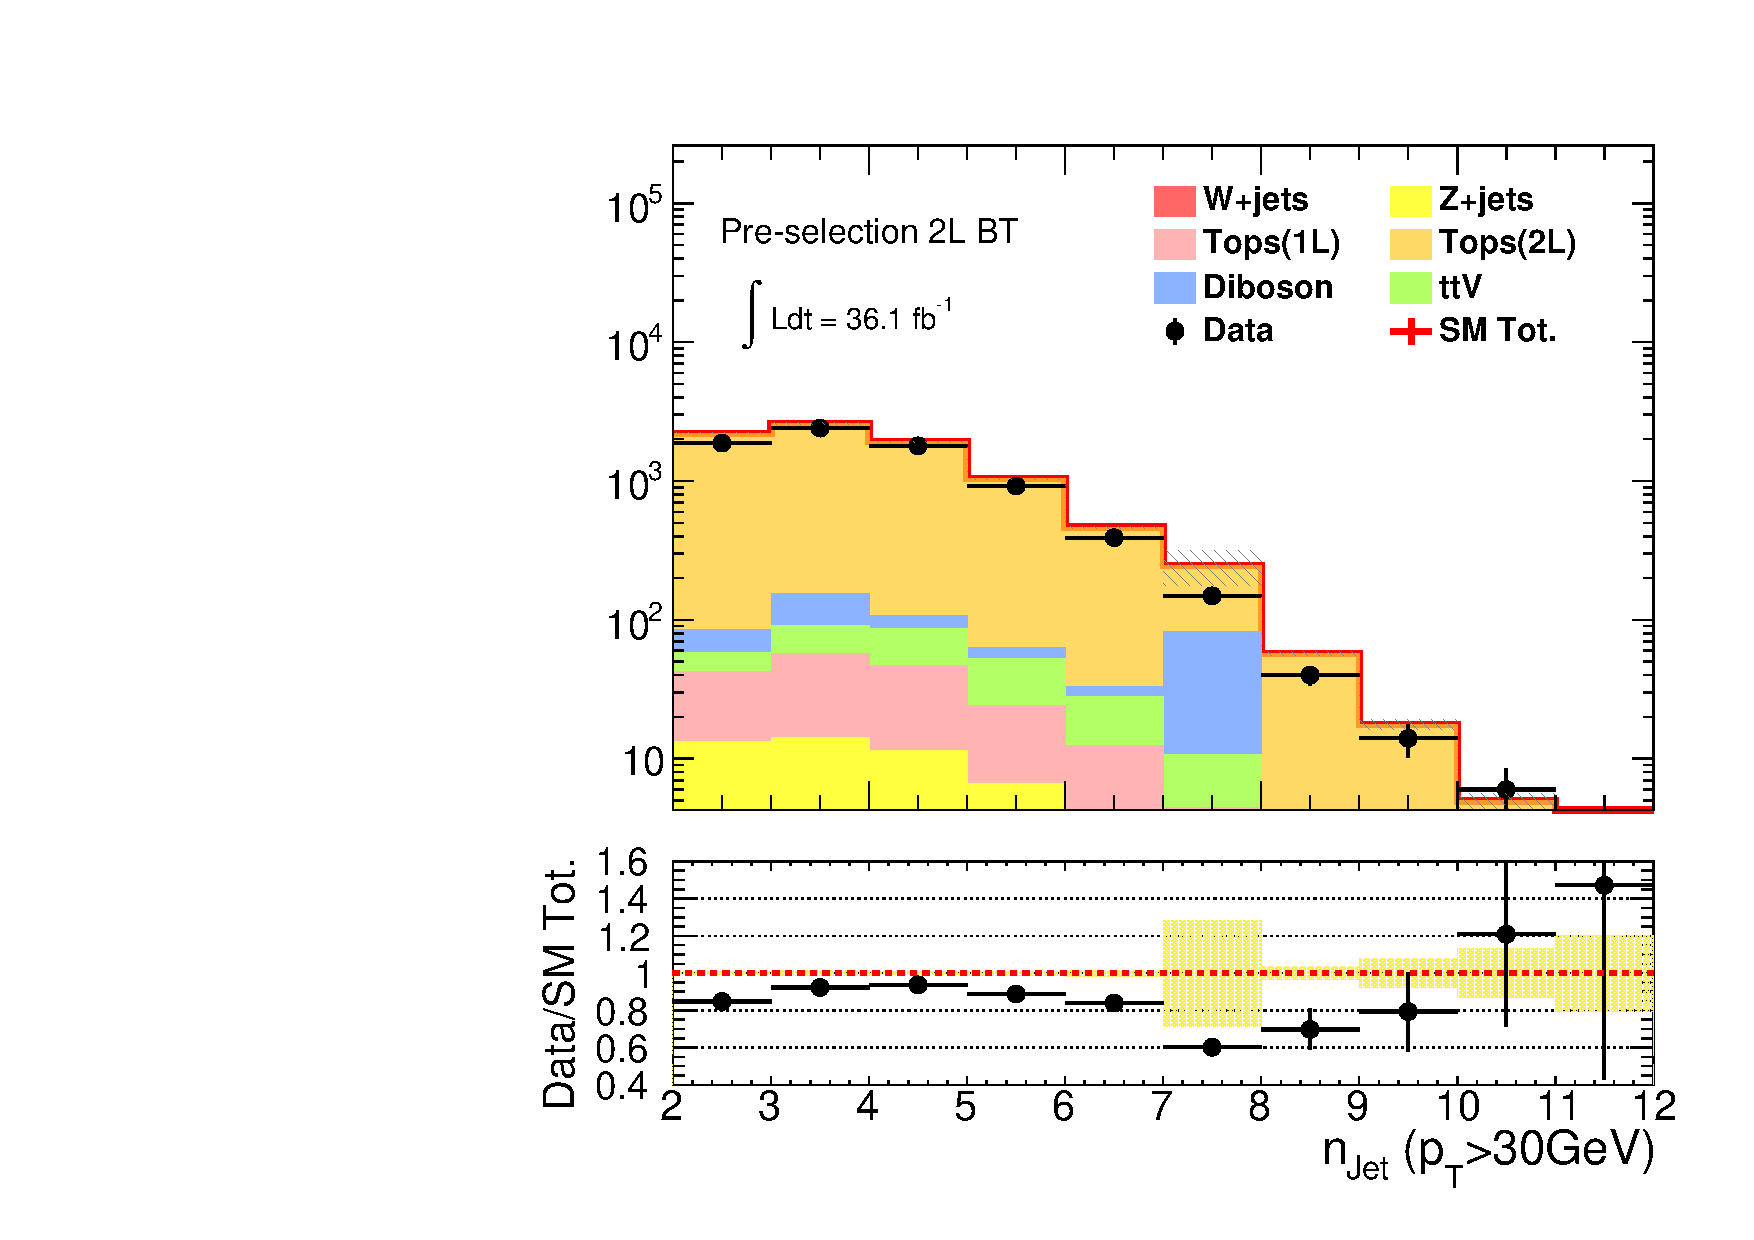
\includegraphics[width=0.48\textwidth]{figures/BGestimation/DataMCComparison/Preselection_2LBT/nJet30__Preselection_2LBT.pdf}}
    \subfigure[]{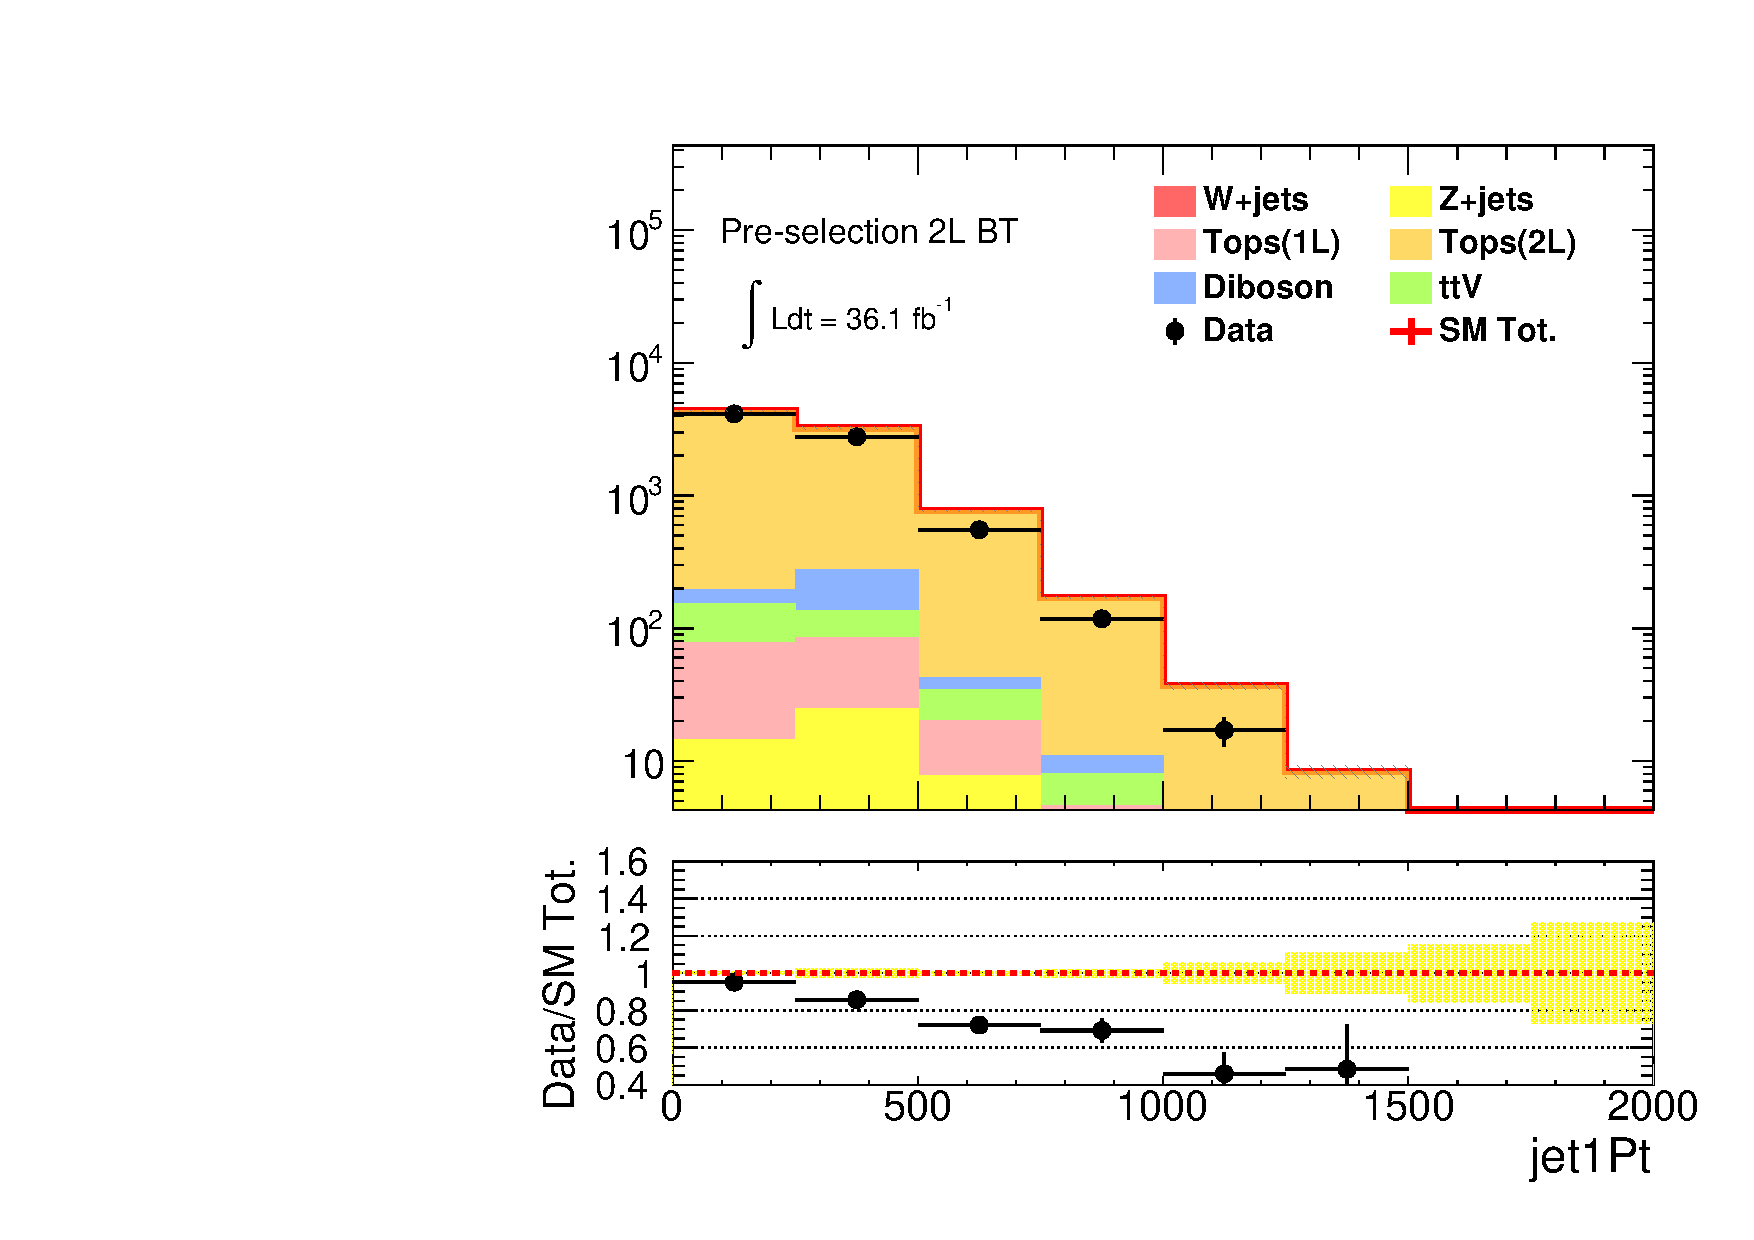
\includegraphics[width=0.48\textwidth]{figures/BGestimation/DataMCComparison/Preselection_2LBT/jet1Pt__Preselection_2LBT.pdf}}
    \subfigure[]{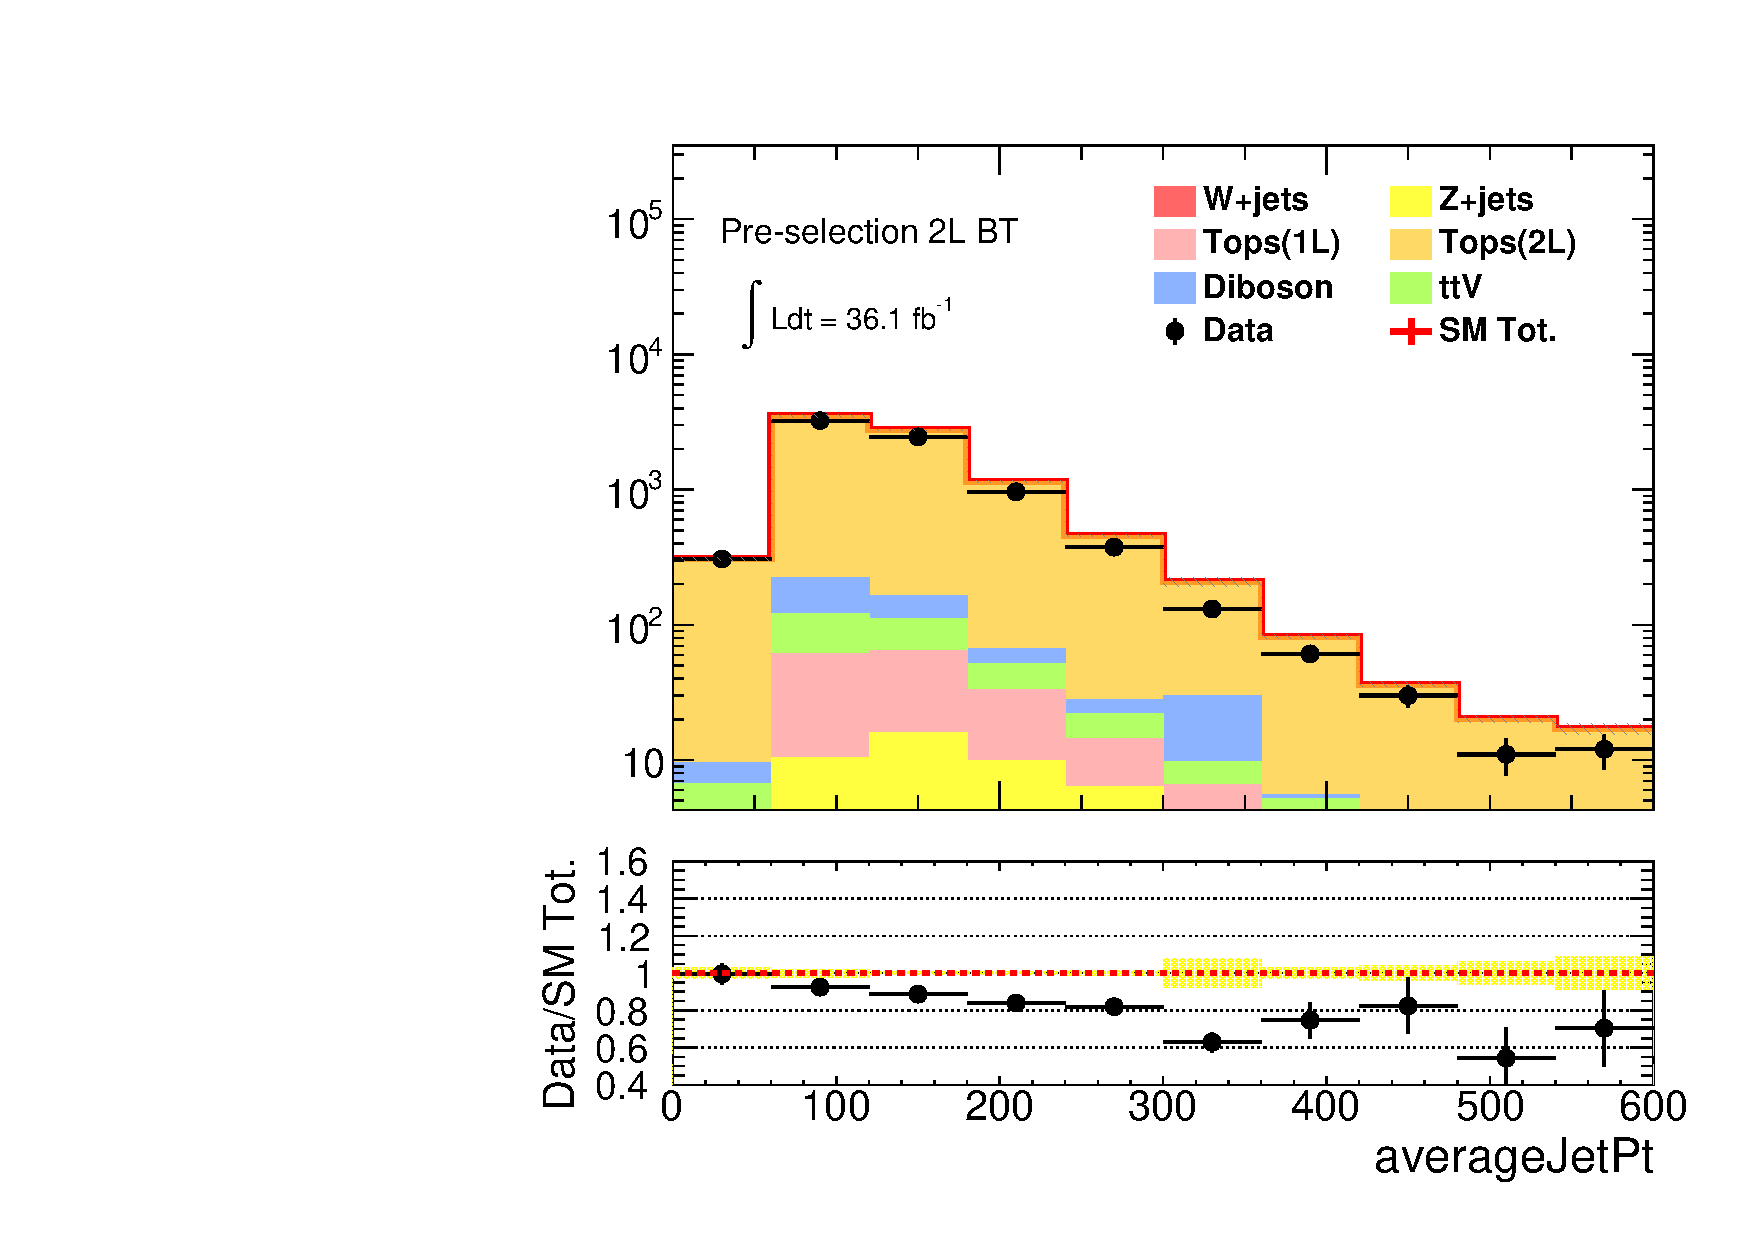
\includegraphics[width=0.48\textwidth]{figures/BGestimation/DataMCComparison/Preselection_2LBT/averageJetPt__Preselection_2LBT.pdf}}
    \subfigure[]{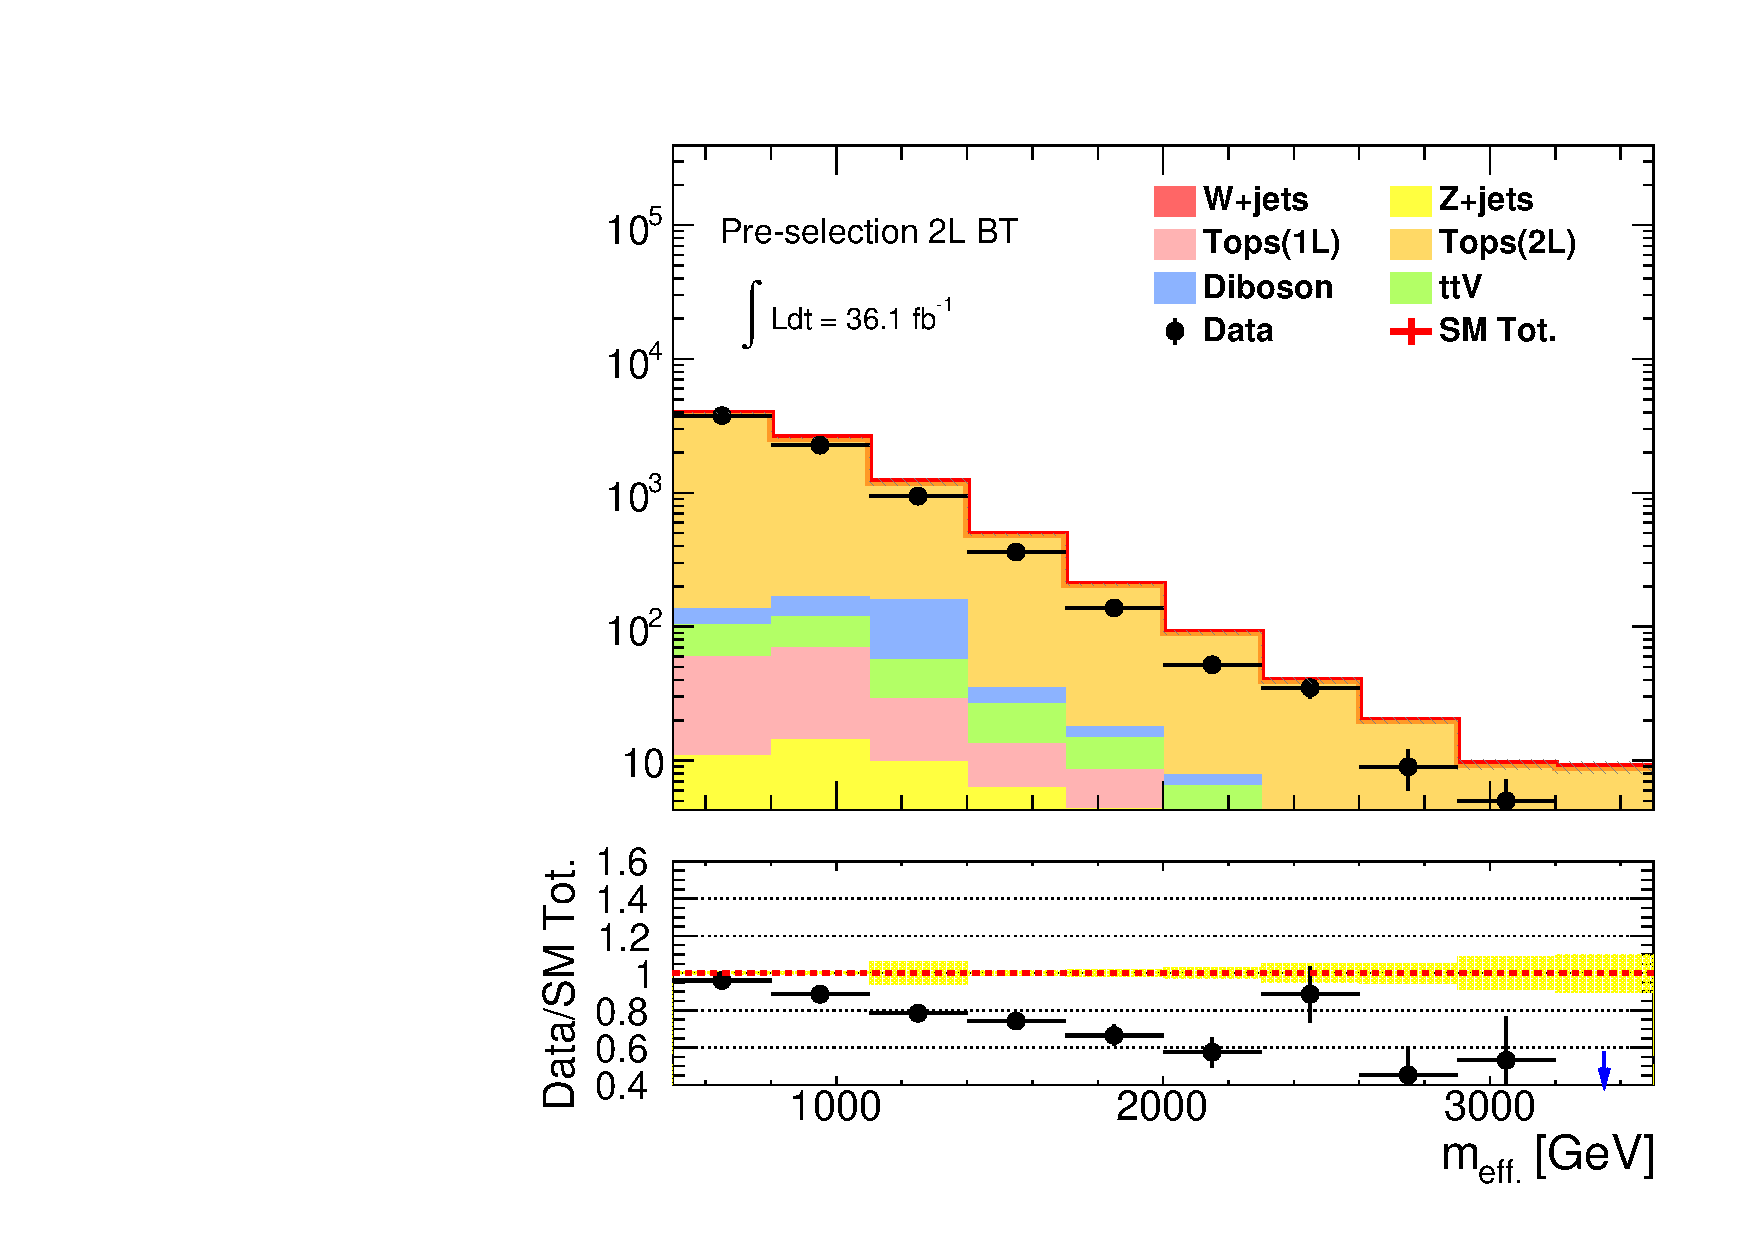
\includegraphics[width=0.48\textwidth]{figures/BGestimation/DataMCComparison/Preselection_2LBT/meffInc30__Preselection_2LBT.pdf}}
    \caption{ Kinematical distribution of (a) Jet multiplicity ($p_T>30\gev$) (b) leading-jet pt  (c) average jet pt ($p_T>30\gev$)  (d) $\meffInc$ in the hard lepton b-tagged pre-selection region.  \label{fig::BGestimation::DataMCPresel2LBT1} }
\end{figure}

\begin{figure}[h]
  \centering
    \subfigure[]{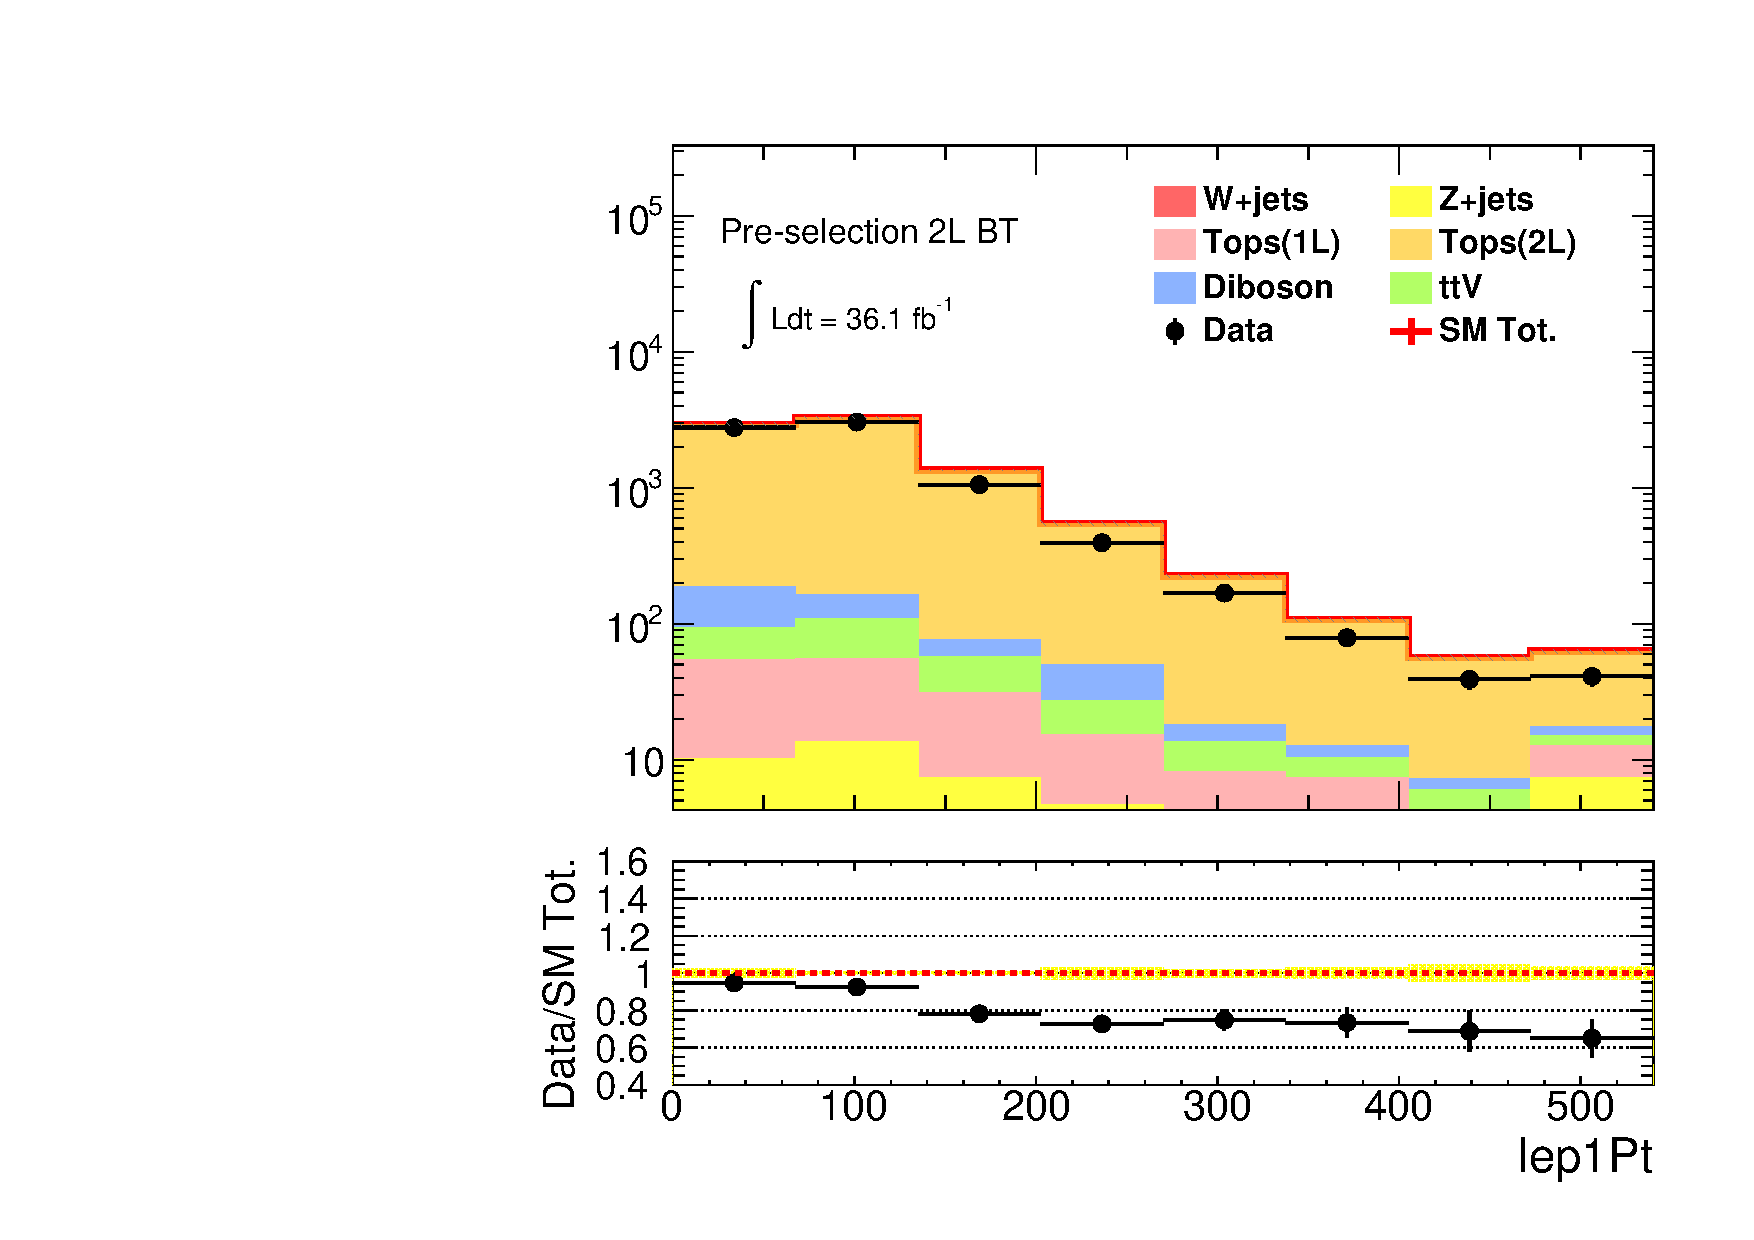
\includegraphics[width=0.48\textwidth]{figures/BGestimation/DataMCComparison/Preselection_2LBT/lep1Pt__Preselection_2LBT.pdf}}
    \subfigure[]{\includegraphics[width=0.48\textwidth]{figures/BGestimation/DataMCComparison/Preselection_2LBT/met__Preselection_2LBT.pdf}}
    \subfigure[]{\includegraphics[width=0.48\textwidth]{figures/BGestimation/DataMCComparison/Preselection_2LBT/mt__Preselection_2LBT.pdf}}
    \subfigure[]{\includegraphics[width=0.48\textwidth]{figures/BGestimation/DataMCComparison/Preselection_2LBT/LepAplanarity__Preselection_2LBT.pdf}}
    \caption{ Kinematical distribution of (a) leading-lepton pt (b) $\met$  (c) $\mt$  (d) $\apl$ in the hard lepton b-tagged pre-selection region.  \label{fig::BGestimation::DataMCPresel2LBT2} }
\end{figure}
%%%%%%%%%%%%%

\begin{figure}[h]
  \centering
    \subfigure[]{\includegraphics[width=0.48\textwidth]{figures/BGestimation/DataMCComparison/Preselection_2LBT/nJet30__Preselection_2LBT__rwgt_nJ007_ttPt007.pdf}}
    \subfigure[]{\includegraphics[width=0.48\textwidth]{figures/BGestimation/DataMCComparison/Preselection_2LBT/jet1Pt__Preselection_2LBT__rwgt_nJ007_ttPt007.pdf}}
    \subfigure[]{\includegraphics[width=0.48\textwidth]{figures/BGestimation/DataMCComparison/Preselection_2LBT/averageJetPt__Preselection_2LBT__rwgt_nJ007_ttPt007.pdf}}
    \subfigure[]{\includegraphics[width=0.48\textwidth]{figures/BGestimation/DataMCComparison/Preselection_2LBT/meffInc30__Preselection_2LBT__rwgt_nJ007_ttPt007.pdf}}
    \caption{ Kinematical distribution of (a) Jet multiplicity ($p_T>30\gev$) (b) leading-jet pt  (c) average jet pt ($p_T>30\gev$)  (d) $\meffInc$ in the hard lepton b-tagged pre-selection region, with the reweighting: $w = 1.05 \times \left[ 1 - 0.061 \,\times p_T(\ttbar) \right]$ (Eq.(\ref{eq::BGestimation::rwgt_ttPt})) being applied for $\ttbar$ MC.  \label{fig::BGestimation::DataMCPresel2LBT_rwgt1} }
\end{figure}

\begin{figure}[h]
  \centering
    \subfigure[]{\includegraphics[width=0.48\textwidth]{figures/BGestimation/DataMCComparison/Preselection_2LBT/lep1Pt__Preselection_2LBT__rwgt_nJ007_ttPt007.pdf}}
    \subfigure[]{\includegraphics[width=0.48\textwidth]{figures/BGestimation/DataMCComparison/Preselection_2LBT/met__Preselection_2LBT__rwgt_nJ007_ttPt007.pdf}}
    \subfigure[]{\includegraphics[width=0.48\textwidth]{figures/BGestimation/DataMCComparison/Preselection_2LBT/mt__Preselection_2LBT__rwgt_nJ007_ttPt007.pdf}}
    \subfigure[]{\includegraphics[width=0.48\textwidth]{figures/BGestimation/DataMCComparison/Preselection_2LBT/LepAplanarity__Preselection_2LBT__rwgt_nJ007_ttPt007.pdf}}
    \caption{ Kinematical distribution of (a) leading-lepton pt (b) $\met$  (c) $\mt$  (d) $\apl$ in the hard lepton b-tagged pre-selection region, with the reweighting: $w = 1.05 \times \left[ 1 - 0.061 \,\times p_T(\ttbar) \right]$ (Eq.(\ref{eq::BGestimation::rwgt_ttPt})) being applied for $\ttbar$ MC.  \label{fig::BGestimation::DataMCPresel2LBT_rwgt2} }
\end{figure}
%%%%%%%%%%%%%

\clearpage

In contrast to variables that scale with transverse momenta of outgoing particles, $\mt$ and aplanarity look relatively well-modeled among ones used in signal regions definition. Therefore, the same estimation strategy is taken as the case of $\wjets$, which is namely extrapolating in these variables from control regions to signal regions. 
However, note that the modeling of $\mt$ is still not as perfect. For instance in Figurere \ref{fig::BGestimation::DataMCPreselHardBV2} or \ref{fig::BGestimation::DataMCPreselHardBV_rwgt2}, there is a small bump-like structure in the ratio plot around $\mt = 100\sim200\gev$ corresponding the cut-off of the semi-leptonic $\ttbar$. 
This is suspected to be due to the interference between $\ttbar+Wt\ra WWbb$ and other $WWbb$ diagrames which is not accounted by the generator, which effect is addressing in regions where bulk $\ttbar$ amplitude is suppressed. Corresponding uncertainty is evaluated in Sec. \ref{sec:Uncertainties::normalizedBG} and assigned as theory systematics. \\

$\mt$ in the bulk di-leptonic component suffers from another issue: while the tail in the $\mt$ distribution of $\wjets$ is only determined by jet energy resolution and the mass-line of W-boson, that of $\ttbar$ is dominated by the di-leptonic component whose $\mt$ simply scales with lepton transverse momentum and MET without any cut-off structure. As a result, the $\mt$ distribution of di-leptonic $\ttbar$ is affected by the mis-modeling rather more severely than the semi-leptonic component in general. The emerged data/MC discrepancy can be seen in Figurere \ref{fig::BGestimation::DataMCPresel2LBT2} (c). \\

To avoid the impact by the mis-modeling in $\mt$, in this analysis di-leptonic components are decided to be estimated by the other ``object replacement'' method as much as possible, and only small portion (``Out Acc.'' and ``Mis. OR'' in Table \ref{tab::BGestimation::BGclass}) of them is covered by the kinematical extrapolation. \\



%%%%%%%%%%%%%
Modeling of $tt+cc/bb$ and $\ttbarFakeB$ are exclusively examined using a preselected region with 3 or more b-jets (\textbf{1L3B}). Figurere \ref{fig::BGestimation::DataMCPresel3B_rwgt1} - \ref{fig::BGestimation::DataMCPresel3B_rwgt2} displays the data-vs-MC comparison in the region. While the shapes seem to be affected by the same type of mis-modeling as observed in inclusive $\ttbar$ selection above, the normalization is also underestimated by about $20\%$ which is thought to be due to the modeling error of $\ttbar+cc/bb$ cross-section. \\

Reweighting function
\begin{align}
w = 1.4 \times \left[ 1 - 0.061 \,\times p_T(\ttbar) \right] \label{eq::BGestimation::rwgt_ttPt3B},
\end{align}
is found to well correct the discrepancy, in which only the normalization coefficiency varies from Eq. \ref{eq::BGestimation::rwgt_ttPt} accounting for the cross-section correctioin for $tt+cc/bb$. Meanwhile, the invariance of the slope coefficiency implies that the source of the shape mis-modeling is common to the bulk $\ttbar$ component as seen above. \\

Despite the $\ttbar$ components in 3B regions suffer from such even more complex mis-modeling than the bulk, the impact on the final result is not dramatic since the majority of them are di-leptonic components in the signal regions which can be estimated largely by the object replacement method.


\begin{figure}[h]
  \centering
    \subfig{0.39}{figures/BGestimation/DataMCComparison/Preselection_3B/nJet30__Preselection_3B.pdf}{Jet multiplicity}
    \subfig{0.39}{figures/BGestimation/DataMCComparison/Preselection_3B/jet1Pt__Preselection_3B.pdf}{$\pt$ of the leading jet}
    \subfig{0.39}{figures/BGestimation/DataMCComparison/Preselection_3B/averageJetPt__Preselection_3B.pdf}{Average $\pt$ of jets with $\pt>30\gev$}
    \subfig{0.39}{figures/BGestimation/DataMCComparison/Preselection_3B/meffInc30__Preselection_3B.pdf}{$\meffInc (\meffDef)$}
    \subfig{0.39}{figures/BGestimation/DataMCComparison/Preselection_3B/lep1Pt__Preselection_3B.pdf}{Lepton's $\pt$}
    \subfig{0.39}{figures/BGestimation/DataMCComparison/Preselection_3B/met__Preselection_3B.pdf}{$\met$}
    \caption{ Kinematical distribution of data (black dots) and MC (colored stack) in the \textbf{1L3B} pre-selection region.  \label{fig::BGestimation::DataMCPresel3B1} }
\end{figure}

\begin{figure}[h]
  \centering
    \subfig{0.48}{figures/BGestimation/DataMCComparison/Preselection_3B/mt__Preselection_3B.pdf}{$\mt$}
    \subfig{0.48}{figures/BGestimation/DataMCComparison/Preselection_3B/LepAplanarity__Preselection_3B.pdf}{$\Apl$}
    \subfig{0.48}{figures/BGestimation/DataMCComparison/Preselection_3B/min_dPhi_4j__Preselection_3B.pdf}{$\mindPhiFourJet$}
    \subfig{0.48}{figures/BGestimation/DataMCComparison/Preselection_3B/topNess__Preselection_3B.pdf}{Topness}
    \caption{ Kinematical distribution of data (black dots) and MC (colored stack) in the \textbf{1L3B} pre-selection region.  \label{fig::BGestimation::DataMCPresel3B2} }
\end{figure}


\begin{figure}[h]
  \centering
    \subfigure[]{\includegraphics[width=0.48\textwidth]{figures/BGestimation/DataMCComparison/Preselection_3B/nJet30__Preselection_3B__rwgt_ttPt007.pdf}}
    \subfigure[]{\includegraphics[width=0.48\textwidth]{figures/BGestimation/DataMCComparison/Preselection_3B/jet1Pt__Preselection_3B__rwgt_ttPt007.pdf}}
    \subfigure[]{\includegraphics[width=0.48\textwidth]{figures/BGestimation/DataMCComparison/Preselection_3B/averageJetPt__Preselection_3B__rwgt_ttPt007.pdf}}
    \subfigure[]{\includegraphics[width=0.48\textwidth]{figures/BGestimation/DataMCComparison/Preselection_3B/meffInc30__Preselection_3B__rwgt_ttPt007.pdf}}
    \caption{ Kinematical distribution of (a) Jet multiplicity ($p_T>30\gev$) (b) leading-jet pt  (c) average jet pt ($p_T>30\gev$)  (d) $\meffInc$ in the \textbf{3b-tagged pre-selection region}, with the reweighting $w = 1.4 \times \left[ 1 - 0.061 \,\times p_T(\ttbar) \right]$ (Eq.(\ref{eq::BGestimation::rwgt_ttPt3B})) being applied for $\ttbar$ MC.  \label{fig::BGestimation::DataMCPresel3B_rwgt1} }
\end{figure}

\begin{figure}[h]
  \centering
    \subfigure[]{\includegraphics[width=0.48\textwidth]{figures/BGestimation/DataMCComparison/Preselection_3B/lep1Pt__Preselection_3B__rwgt_ttPt007.pdf}}
    \subfigure[]{\includegraphics[width=0.48\textwidth]{figures/BGestimation/DataMCComparison/Preselection_3B/met__Preselection_3B__rwgt_ttPt007.pdf}}
    \subfigure[]{\includegraphics[width=0.48\textwidth]{figures/BGestimation/DataMCComparison/Preselection_3B/mt__Preselection_3B__rwgt_ttPt007.pdf}}
    \subfigure[]{\includegraphics[width=0.48\textwidth]{figures/BGestimation/DataMCComparison/Preselection_3B/LepAplanarity__Preselection_3B__rwgt_ttPt007.pdf}}
    \caption{ Kinematical distribution of (a) leading-lepton pt (b) $\met$  (c) $\mt$  (d) $\apl$ in the \textbf{3b-tagged pre-selection region}, with the reweighting: $w = 1.4 \times \left[ 1 - 0.061 \,\times p_T(\ttbar) \right]$ (Eq.(\ref{eq::BGestimation::rwgt_ttPt3B})) being applied for $\ttbar$ MC.  \label{fig::BGestimation::DataMCPresel3B_rwgt2} }
\end{figure}

%\begin{figure}[h]
%  \centering
%    \subfigure[]{\includegraphics[width=0.48\textwidth]{figures/BGestimation/DataMCComparison/Preselection_3B/min_dPhi_4j__Preselection_3B__rwgt_ttPt007.pdf}}
%    \subfigure[]{\includegraphics[width=0.48\textwidth]{figures/BGestimation/DataMCComparison/Preselection_3B/topNess__Preselection_3B__rwgt_ttPt007.pdf}}
%    \caption{ Kinematical distribution of (a) $\mindPhiFourJet$ (b) $\topNess$ in the  3b-tagged pre-selection region.  \label{fig::BGestimation::DataMCPresel3B3} }
%\end{figure}


\clearpage


%\subsubsection{Dibosons}
%\begin{figure}[h]
  \centering
    \subfigure[]{\includegraphics[width=0.48\textwidth]{figures/BGestimation/DataMCComparison/Preselection_2LDB/nJet30__Preselection_2LDB.pdf}}
    \subfigure[]{\includegraphics[width=0.48\textwidth]{figures/BGestimation/DataMCComparison/Preselection_2LDB/jet1Pt__Preselection_2LDB.pdf}}
    \subfigure[]{\includegraphics[width=0.48\textwidth]{figures/BGestimation/DataMCComparison/Preselection_2LDB/averageJetPt__Preselection_2LDB.pdf}}
    \subfigure[]{\includegraphics[width=0.48\textwidth]{figures/BGestimation/DataMCComparison/Preselection_2LDB/meffInc30__Preselection_2LDB.pdf}}
    \caption{ Kinematical distribution of (a) Jet multiplicity ($p_T>30\gev$) (b) leading-jet pt  (c) average jet pt ($p_T>30\gev$)  (d) $\meffInc$ in the hard lepton b-tagged pre-selection region.  \label{fig::BGestimation::DataMCPresel2LDB1} }
\end{figure}

\begin{figure}[h]
  \centering
    \subfigure[]{\includegraphics[width=0.48\textwidth]{figures/BGestimation/DataMCComparison/Preselection_2LDB/lep1Pt__Preselection_2LDB.pdf}}
    \subfigure[]{\includegraphics[width=0.48\textwidth]{figures/BGestimation/DataMCComparison/Preselection_2LDB/met__Preselection_2LDB.pdf}}
    \subfigure[]{\includegraphics[width=0.48\textwidth]{figures/BGestimation/DataMCComparison/Preselection_2LDB/mt__Preselection_2LDB.pdf}}
    \subfigure[]{\includegraphics[width=0.48\textwidth]{figures/BGestimation/DataMCComparison/Preselection_2LDB/LepAplanarity__Preselection_2LDB.pdf}}
    \caption{ Kinematical distribution of (a) leading-lepton pt (b) $\met$  (c) $\mt$  (d) $\apl$ in the hard lepton b-tagged pre-selection region.  \label{fig::BGestimation::DataMCPresel2LDB2} }
\end{figure}
%%%%%%%%%%%%%

%\begin{figure}[h]
  \centering
    \subfigure[]{\includegraphics[width=0.48\textwidth]{figures/BGestimation/DataMCComparison/Preselection_2LDB/nJet30__Preselection_2LDB__rwgt_nJ007_ttPt007.pdf}}
    \subfigure[]{\includegraphics[width=0.48\textwidth]{figures/BGestimation/DataMCComparison/Preselection_2LDB/jet1Pt__Preselection_2LDB__rwgt_nJ007_ttPt007.pdf}}
    \subfigure[]{\includegraphics[width=0.48\textwidth]{figures/BGestimation/DataMCComparison/Preselection_2LDB/averageJetPt__Preselection_2LDB__rwgt_nJ007_ttPt007.pdf}}
    \subfigure[]{\includegraphics[width=0.48\textwidth]{figures/BGestimation/DataMCComparison/Preselection_2LDB/meffInc30__Preselection_2LDB__rwgt_nJ007_ttPt007.pdf}}
    \caption{ Kinematical distribution of (a) Jet multiplicity ($p_T>30\gev$) (b) leading-jet pt  (c) average jet pt ($p_T>30\gev$)  (d) $\meffInc$ in the hard lepton b-tagged pre-selection region.  \label{fig::BGestimation::DataMCPresel2LDB1} }
\end{figure}

\begin{figure}[h]
  \centering
    \subfigure[]{\includegraphics[width=0.48\textwidth]{figures/BGestimation/DataMCComparison/Preselection_2LDB/lep1Pt__Preselection_2LDB__rwgt_nJ007_ttPt007.pdf}}
    \subfigure[]{\includegraphics[width=0.48\textwidth]{figures/BGestimation/DataMCComparison/Preselection_2LDB/met__Preselection_2LDB__rwgt_nJ007_ttPt007.pdf}}
    \subfigure[]{\includegraphics[width=0.48\textwidth]{figures/BGestimation/DataMCComparison/Preselection_2LDB/mt__Preselection_2LDB__rwgt_nJ007_ttPt007.pdf}}
    \subfigure[]{\includegraphics[width=0.48\textwidth]{figures/BGestimation/DataMCComparison/Preselection_2LDB/LepAplanarity__Preselection_2LDB__rwgt_nJ007_ttPt007.pdf}}
    \caption{ Kinematical distribution of (a) leading-lepton pt (b) $\met$  (c) $\mt$  (d) $\apl$ in the hard lepton b-tagged pre-selection region.  \label{fig::BGestimation::DataMCPresel2LDB2} }
\end{figure}
%%%%%%%%%%%%%



\subsubsection{Definition of Control Regions and Validation Regions} \label{sec::BGestimation::CRdef}
The key assumption in this method is that the relative modeling of MC between CRs and SRs are correct. In other words, both CRs and SRs suffer from the same mis-modeling, so that the normalization factor measured in CR is applicable to SR. Therefore, the most important requirement in CR definition is having the similar phase space with respect to corresponding SR in terms of the mis-modeling. \\

The easiest realization of CR is to revert the SR cuts in kinematical variables that are well-modeled by MC. In this analysis, $\mt$, $\apl$ and topness (and also $\mindPhiFourJet$ for the ``3B'' tower) are chosen as the baseline extrapolation variables. 
A exception is in the``2J'' tower where $\met$ is used instead of aplanarity, since it is not used in the signal regions selection.
%since aplanarity is not used in definition. 
%The modeling of $\met$ is acceptable, since the ISR/FSR conribution in the ``2J'' tower is relatively low due to the loose selection in number of jets. \\ \\
%topness, min_dPhi_4j

A couple of minor modifications follow based on following supplemental requirements:
\begin{itemize}
\item CR statistics have to be sufficient. \\
Typically, about 10 times more data statistics in CRs with respect to SRs are desired to make the correction stable particularly in cases where multiple components are corrected simultaneously (in this analysis, $\wjets$ and $\ttbar+Wt$). 
For this sake, cuts in variables fatally sensitive to the mis-modeling is loosened in some of the CRs, even at some cost of being hit by the mis-modeling.
MET is for example always a good candidate to loosen since the gain in statistics increase is large.
Although it is affected by the mis-modeling through jet transverse momenta which is known to be the most ill-modeled, 
the influence is much diluted through the vectoral summation of them, instead of the scalar sum. 
$\metOverMeff$ is also loosened in ``2J'' and ``High-x'' since it is in a form of ratio which is supposed to be robust against simultaneous variation of the enumerator and the denominator.
The impact by the mis-modeling due to these loosened cuts are evaluated in Sec \ref{sec::BGestimation::nonClosure_kineExtp}.
On the other hand, it is promissed that $\nJet$ and $\meffInc$ are never touched since they are critical to the mis-modeling. \\
%
\item Lower cut in $\mt$ to reduce the contribution from fake leptons. \\
Low-$\mt$ regions are typically have higher abundance of events with fake leptons for $\wjets$ and $\ttbar$.
As the MC modeling on the fake rate is generally less reliable, $\mt > 30 \sim 40 \gev$ is applied in CR to get rid of the influence. 
\end{itemize}

CRs are defined for each tower and $\meffInc$ bins independently, however are shared between b-tagged and b-vetoed SR bins.  Normalization is applied only on $\wjets$, $\ttbar$ and single-top while raw MC prediction is quoted for diboson and the other minor backgrounds. $\ttbar$ and single-top share the normalization factors as their relative breakdown is similar in CRs and SRs. 
%definition of ``tops''
The normalization factors are determined by a simultaneous fit on the b-vetoed and b-tagged slice of a CR (``WR'' and ``TR'') in which $\wjets$ and $\ttbar$ is dominant respectively. During the fit, all the normalization factors and nuisance parameters characterizing theoretical and experimental systematics are allowed to flow. The detail of the statistical procedure is described in Sec. \ref{sec::Result::statistics}. \\

There are the third type of regions referred as ``validation regions'' designed to confirm the validity of the background estimation procedure by comparing with the data. They are typically set in between the CR and SR, with the cut in one of the extrapolation variable is freed with respect to CRs and kept for the other one. VRa and VRb respectively validates the extrapolation in $\mt$ and $\apl$ ($\met$ for ``2J''). Upper cut on $\mt$ is set in some VRa to suppress the signal contamination. VRs-QCD are the regions to examine the contribution from QCD multi-jet processes in SRs which is supposedly negligible. The detail is found in Sec. \ref{sec::BGestimation::VRQCD}. \\

The finalized CRs and VRs are summarized together with the corresponding SRs in Table \ref{SRdefinition::regionDef2J} - \ref{SRdefinition::regionDef3B}, with the graphical schematics being shown in Figurere \ref{fig::BGestimation::regionsPlot}. While SRs are carefully designed to be orthogonal to CRs and VRs, it is allowed to have overlap between CRs and VRs once the CRs are found to have much larger statistics than that of the VRs so that the overlapped events have no influence to the normalization. For instance, CR adn VRa are overlapped in ``3B''. This is intended to secure the CR statistics, while the number of events in VRa is small enough so that they are still nearly statistically independent. \\
\clearpage

%%%%%%%%%%%%%%%%%%%%
\begin{figure}[h]
  \centering
    \subfigure[]{\includegraphics[width=0.45\textwidth]{figures/BGestimation/regionsPlot/regionsPlot_myAna_2J.pdf}}
    \subfigure[]{\includegraphics[width=0.45\textwidth]{figures/BGestimation/regionsPlot/regionsPlot_myAna_6J.pdf}}
    \subfigure[]{\includegraphics[width=0.45\textwidth]{figures/BGestimation/regionsPlot/regionsPlot_myAna_Lowx.pdf}}
    \subfigure[]{\includegraphics[width=0.45\textwidth]{figures/BGestimation/regionsPlot/regionsPlot_myAna_Highx.pdf}}
    \subfigure[]{\includegraphics[width=0.45\textwidth]{figures/BGestimation/regionsPlot/regionsPlot_myAna_3B.pdf}}
 \caption{ Schematics of CR/VR/SR in each signal region tower. Two major extrapolation variables are chosen to illustrate the difference between the regions. Extrapolation in the other variables are explicitly mentioned in the label. Note that the control region in the ``3B'' tower contains the VRa in it. 
%to boost the CR statistics.
%, which does not disturb the role of validation given that it has 5 times more statistics as that of VRa. 
   \label{fig::BGestimation::regionsPlot} 
 }
\end{figure}

\clearpage

%%%%%%%%%%%%%%%%%%%%%%%%%%%%%%%%%%%%%%%%%%%%%%%%%%%%%%%%%%
%\subsubsection{Signal contamination}
%\input{tex/BGestimation/fig_sigContami_kineExtp.tex}


%%%%%%%%%%%%%%%%%%%%%%%%%%%%%%%%%%%%%%%%%%%%%%%%%%%%%%%%%%
\subsubsection{Evaluation of the Extrapolation Error} \label{sec::BGestimation::nonClosure_kineExtp}
Although the good modeling on the extrapolation variables is confirmed in the pre-selection regions, 
the question is whethere they are still good when the signal region selections are applid.
In fact, there is correlation between the well-modeled variables ($\mt$, $\apl$ etc.) and the ill-modeled ones ($\nJetNoGev$, jet transverse momenta, $\meffInc$ etc.) that are not evident at preselection level, however could be addressing in some particular phase space. 
The extrapolation is also affected by the loosened cuts in variables that are already known to be poorly modeled such as MET, so the associated uncertainty needs be quantified. \\

In this sub-section, the extrapolation error is evaluated by injecting an artificial variation in MC compared to the observed MC mis-modeling, and then measure the yield change in a CR and the corresponding SR. Ideally, they show the same response against the injected variation, so that the normalization in CR can perfectly compensate the effect of mis-modeling in SR. Otherwise, the relative difference in their yield variation directly corresponds to the amount of extrapolation error. \\

Figurere \ref{fig::BGestimation::valid_extp_2J} - \ref{fig::BGestimation::valid_extp_3B} present the results where the $\wjets$ and $\ttbar$ MC are varied by reweighting the events with:
\begin{align}
 w & = 1 - x \times (\nJetNoGev-2), \mbox{\phantom{MMMM}}\,\,\,\,\,\, x \in [0,0.18]  \mbox{\phantom{MMMM}} (\wjets) \nn  \\
 w & = 1 - x \,\times p_T(\ttbar)/100\gev, \,\,\,\,\,\,\,\,           x \in [0,0.09]  \mbox{\phantom{MMMM}} (\ttbar),
\label{eq::BGestimation::injected_MCvariation}
\end{align}
respectively. The vertical axis on the top panels show the amount of relative change that CR or SR experience by the injected MC variation as a function of $x$. The relative variation in CR (orange) compares to the normalization factor actually obtained via the fit to data, while that in SR (blue) to the ideal normalization factor need to fully correct the SR. The bottom panel display the ratio, namely the resultant extrapolation error. The realistic $x$ is approximately $x_W=0.1$ and $x_{\ttbar}=0.06$ for $\wjets$ and $\ttbar$ respectively, based on the observation of data/MC in Sec. \ref{sec::BGestimation::dataMC} as Eq. (\ref{eq::BGestimation::rwgt_nJ}), (\ref{eq::BGestimation::rwgt_ttPt}) and (\ref{eq::BGestimation::rwgt_ttPt3B}). B-tagging requirement is removed to maintain sufficient statistics, assuming the kinematics are invariant with it. For the $\ttbar$ process, component estimated by the object replacement method is excluded from the test. The extrapolation error from CRs to corresponding VRs are shown in Appendix Sec.\ref{sec::App::valid_extp_VR}. \\

Observed extrapolation error is generally small, which stays within 10$\%$ (20$\%$) for $\wjets$ ($\ttbar$) at the reference magnitude of mis-modeling ($x_W=0.1, \,\,\, x_{\ttbar}=0.06$). These are quoted as systematics error associated with the method in the fit, which is summarized in Table \ref{tab::Uncertainties::noClosure_kineExtp} of Sec. \ref{sec::Uncertainties::nonClosure}. \\

%
% note that このtestはmt/apl extraplationで最大のIssueであるjetのMis-modelingがどれくらい解消できるかというtestであり、本質的にmt spectraとmis-modelingがどれくらい相関しているかを見ているにすぎない。
%in other preselectionにおけるmtの記述が完璧だとした場合にjet selectionかけたときにどれくらいmt. aplの分布がズレるかというtestである. 
% 
%このtestでevaluateしたerrorは手法に由来するsystematicとしてassignするが、jet以外の要因によるMT spectraのvariationは別個評価する必要がある. (instrumental, theory etc.)
%これらは7章でevaluateする

Note that this check is only quantifying the error in the methodology; how much the MC mis-modeling in terms of jet activities can be corrected if the other MC description is perfect.
In reality, the shape of $\mt$ or $\apl$ distribution can be varies by the other reasons, and the uncertainties have to be assigned additionally. This will be discussed in Sec. \ref{sec::Uncertainties}.

\clearpage
%\begin{figure}[h]
  \centering
    \subfig{0.48}{figures/BGestimation/valid_extp/SFTF_Wjets_Preselection_meff1500_extp_mt__nJet30.pdf}{}
    \subfig{0.48}{figures/BGestimation/valid_extp/SFTF_Wjets_Preselection_meff1500_extp_LepAplanarity__nJet30.pdf}{}
    \caption{ Closure error for $\wjets$ process by the extrapolation using (a) $\mt$ (b) $\apl$ as function of the magnitude of injected linear mis-modeling on $\nJet$: $y_{\ttbar} = 1.0 - x \times \nJet)$. All evaluated by MC.   \label{fig::BGestimation::valid_extp1} }
\end{figure}

%%%%%%%%%%%%%%%%
\begin{figure}[h]
  \centering
    \subfig{0.48}{figures/BGestimation/valid_extp/SFTF_Wjets_Preselection_meff1500_extp_mt__WPt.pdf}{}
    \subfig{0.48}{figures/BGestimation/valid_extp/SFTF_Wjets_Preselection_meff1500_extp_LepAplanarity__WPt.pdf}{}
    \caption{ Closure error for $\wjets$ process by the extrapolation using (a) $\mt$ (b) $\apl$ as function of the magnitude of injected linear mis-modeling on $\nJet$: $y_{\ttbar} = 1.0 - x \times \nJet)$. All evaluated by MC.   \label{fig::BGestimation::valid_extp2} }
\end{figure}


%%%%%%%%%%%%%%%%
\begin{figure}[h]
  \centering
    \subfig{0.48}{figures/BGestimation/valid_extp/SFTF_tt_Preselection_meff1500_extp_mt__ttPt.pdf}{}
    \subfig{0.48}{figures/BGestimation/valid_extp/SFTF_tt_Preselection_meff1500_extp_LepAplanarity__ttPt.pdf}{}
    \caption{ Closure error for $\ttbar$ process by the extrapolation using (a) $\mt$ (b) $\apl$ as function of the magnitude of injected linear mis-modeling on $p_T(\ttbar)$: $y_{\ttbar} = 1.0 - x \times p_T(\ttbar))$. All evaluated by MC.   \label{fig::BGestimation::valid_extp1} }
\end{figure}

%%%%%%%%%%%%%%%%
\begin{figure}[h]
  \centering
    \subfig{0.48}{figures/BGestimation/valid_extp/SFTF_tt_Preselection_meff1500_extp_mt__meff.pdf}{}
    \subfig{0.48}{figures/BGestimation/valid_extp/SFTF_tt_Preselection_meff1500_extp_LepAplanarity__meff.pdf}{}
    \caption{ Closure error for $\ttbar$ process by the extrapolation using (a) $\mt$ (b) $\apl$ as function of the magnitude of injected linear mis-modeling on $meffInc$: $y_{\ttbar} = 1.0 - x \times \meffInc)$. All evaluated by MC.   \label{fig::BGestimation::valid_extp1} }
\end{figure}



%%%%%%%%%%%%%%%% SR2J
\begin{figure}[h]
  \centering
    \subfigure[]{\includegraphics[width=0.488\textwidth]{figures/BGestimation/valid_extp/SFTF_wjets_SR2JMEFF1_extp_var2J__nJet30.pdf}}
    \subfigure[]{\includegraphics[width=0.488\textwidth]{figures/BGestimation/valid_extp/SFTF_ttNoObjRep_SR2JMEFF1_extp_var2J__ttPt.pdf}}
    \subfigure[]{\includegraphics[width=0.488\textwidth]{figures/BGestimation/valid_extp/SFTF_wjets_SR2JMEFF2_extp_var2J__nJet30.pdf}}
    \subfigure[]{\includegraphics[width=0.488\textwidth]{figures/BGestimation/valid_extp/SFTF_ttNoObjRep_SR2JMEFF2_extp_var2J__ttPt.pdf}}
    \subfigure[]{\includegraphics[width=0.488\textwidth]{figures/BGestimation/valid_extp/SFTF_wjets_SR2JMEFF3_extp_var2J__nJet30.pdf}}
    \subfigure[]{\includegraphics[width=0.488\textwidth]{figures/BGestimation/valid_extp/SFTF_ttNoObjRep_SR2JMEFF3_extp_var2J__ttPt.pdf}}
 \caption{Extrapolation error in SR/CR 2J. B-tagging requirement is removed. Top pannels show the yield variation of (a) $\wjets$ and (b) $\ttbar$ when injecting the variation by reweighting the MC with Eq. \ref{eq::BGestimation::injected_MCvariation}. Bottom rows are the relative difference in their response against the injected variation, namely the extrapolation errir. For the $\ttbar$ process, component estimated by the object replacement method is removed.  \label{fig::BGestimation::valid_extp_2J} }
\end{figure}



%%%%%%%%%%%%%%%% SR6J
\begin{figure}[h]
  \centering
    \subfigure[]{\includegraphics[width=0.488\textwidth]{figures/BGestimation/valid_extp/SFTF_wjets_SR6JMEFF1_extp_var6J__nJet30.pdf}}
    \subfigure[]{\includegraphics[width=0.488\textwidth]{figures/BGestimation/valid_extp/SFTF_ttNoObjRep_SR6JMEFF1_extp_var6J__ttPt.pdf}}
    \subfigure[]{\includegraphics[width=0.488\textwidth]{figures/BGestimation/valid_extp/SFTF_wjets_SR6JMEFF2_extp_var6J__nJet30.pdf}}
    \subfigure[]{\includegraphics[width=0.488\textwidth]{figures/BGestimation/valid_extp/SFTF_ttNoObjRep_SR6JMEFF2_extp_var6J__ttPt.pdf}}
    \subfigure[]{\includegraphics[width=0.488\textwidth]{figures/BGestimation/valid_extp/SFTF_wjets_SR6JMEFF3_extp_var6J__nJet30.pdf}}
    \subfigure[]{\includegraphics[width=0.488\textwidth]{figures/BGestimation/valid_extp/SFTF_ttNoObjRep_SR6JMEFF3_extp_var6J__ttPt.pdf}}
 \caption{Extrapolation error in SR/CR 6J. B-tagging requirement is removed. Top pannels show the yield variation of (a) $\wjets$ and (b) $\ttbar$ when injecting the variation by reweighting the MC with Eq. \ref{eq::BGestimation::injected_MCvariation}. Bottom rows are the relative difference in their response against the injected variation, namely the extrapolation errir. For the $\ttbar$ process, component estimated by the object replacement method is removed.  \label{fig::BGestimation::valid_extp_6J} }
\end{figure}


%%%%%%%%%%%%%%%% Lowx
\begin{figure}[h]
  \centering
    \subfigure[]{\includegraphics[width=0.488\textwidth]{figures/BGestimation/valid_extp/SFTF_wjets_SRLowx_extp_varLowx__nJet30.pdf}}
    \subfigure[]{\includegraphics[width=0.488\textwidth]{figures/BGestimation/valid_extp/SFTF_ttNoObjRep_SRLowx_extp_varLowx__ttPt.pdf}}

%%%%%%%%%%%%%%%% Highx
    \subfigure[]{\includegraphics[width=0.488\textwidth]{figures/BGestimation/valid_extp/SFTF_wjets_SRHighx_extp_varHighx__nJet30.pdf}}
    \subfigure[]{\includegraphics[width=0.488\textwidth]{figures/BGestimation/valid_extp/SFTF_ttNoObjRep_SRHighx_extp_varHighx__ttPt.pdf}}
 \caption{Extrapolation error in SR/CR (a)(b) Low-x, and (c)(d) High-x. B-tagging requirement is removed. Top pannels show the yield variation of $\wjets$ (left) and $\ttbar$ (right) when injecting the variation by reweighting the MC with Eq. \ref{eq::BGestimation::injected_MCvariation}. Bottom rows are the relative difference in their response against the injected variation, namely the extrapolation errir. For the $\ttbar$ process, component estimated by the object replacement method is removed.  \label{fig::BGestimation::valid_extp_6J} }
\end{figure}


%%%%%%%%%%%%%%%% 3B
\begin{figure}[h]
  \centering
    \subfigure[]{\includegraphics[width=0.488\textwidth]{figures/BGestimation/valid_extp/SFTF_wjets_SR3BMEFF1_extp_var3B__nJet30.pdf}}
    \subfigure[]{\includegraphics[width=0.488\textwidth]{figures/BGestimation/valid_extp/SFTF_ttNoObjRep_SR3BMEFF1_extp_var3B__ttPt.pdf}}
    \subfigure[]{\includegraphics[width=0.488\textwidth]{figures/BGestimation/valid_extp/SFTF_wjets_SR3BMEFF2_extp_var3B__nJet30.pdf}}
    \subfigure[]{\includegraphics[width=0.488\textwidth]{figures/BGestimation/valid_extp/SFTF_ttNoObjRep_SR3BMEFF2_extp_var3B__ttPt.pdf}}
 \caption{Extrapolation error in SR/CR 3B. B-tagging requirement is removed for $\wjets$. Top pannels show the yield variation of $\wjets$ (left) and $\ttbar$ (right) when injecting the variation by reweighting the MC with Eq. \ref{eq::BGestimation::injected_MCvariation}. Bottom rows are the relative difference in their response against the injected variation, namely the extrapolation errir. For the $\ttbar$ process, component estimated by the object replacement method is removed.  \label{fig::BGestimation::valid_extp_3B} }
\end{figure}







\clearpage

%%%%%%%%%%%%%%%%%%%%%%%%%%%%%%%%%%%%%%%%%%%%%%%%%%%%%%%%%%
\subsubsection{Result of Backgroun-only Fit} \label{sec::BGestimation::kineExtp::result}
The data yields in control regions are summarized in Table\ref{tab::BGestimation::CRyields_2J} - \ref{tab::BGestimation::CRyields_3B}, accompanied with the pre-fit and post-fit prediction by MC. Note that only $\wjets$ and top backgrounds ($\ttbar$ and single-top) are normalized and the yield of other processes are kept during the fit. The effect of signal contamination in control regions is neglected therefore referred as ``background-only fit''. \\

Fitted normalization factors are summarized in Figurere \ref{fig::BGestimation::fittedSFs}. Generally they decrease with elevating $\meffInc$-bin, consistent to the data-MC observation where MC is systematically over-predict in high $\meffInc$ regions.


\clearpage
%どのregionでもreweightingで修正したものと大体一致
%reweightingがhard-seelection掛けた後のphase spaceでのmis-modelingもcatchできていることの証明
%上でも言ったが一番大事なのはmis modelingがなんのせいかある程度把握してるということ。
%逆に一番やばいのは複数の逆にcontributeしてるmis-modelingがキャンセルすること。
%なのでCR fitの小さいNormalizaiton factorというのは確かにdisasterではあるが、
%このnJet rwgtだけで大体の説明がついてしまうというのはかなり良い兆候で、仮にcalcelする成分が仮にいたとしてもnJetのMis-modelingに比べれば大したことがないということが言える

Figurere \ref{fig::BGestimation::CRpostFit::WR2J}-\ref{fig::BGestimation::CRpostFit::TR3B} are the post-fit distributions for variables used in the extrapolation in each region. Blue arrows indicate the CRs that the MC is normalized. 
% data/MCにdescrepancy trendが見られるものがチラホラある
%
% 2JのMET


%
% W+jetsもttbarもmtが若干怪しい
%


%---------------------- Fitted normalization factors ------------------- 
\begin{figure}[h]
  \begin{center}
    \includegraphics[width=160mm]{figures/BGestimation/fittedSFs/SFs.pdf}
    \captionof{figure}{Fitted normalization factors for $\wjets$ and top backgrounds ($\ttbar$ plus single-top). The error bars represent combined systematic and statistical uncertainties. }
    \label{fig::BGestimation::fittedSFs}
  \end{center}
\end{figure}
%-------------------------------

\clearpage
\newcommand{\crtablecaption}[1]{%
      Number of observed data and the estimated background yields in the control regions in tower \textbf{#1}. 
      Uncertainties include both systematic uncertainties discussed in chapter \ref{sec::Uncertainties} and the uncertainties due to the limited data statistics in CR or the MC statistics. 
      The uncertainties are symmetrised and truncated so that the yields remain positive.
}

\begin{table}
  \begin{center}
    \caption{ \label{tab::BGestimation::CRyields_2J} \crtablecaption{2J}  }

    \begin{tabular*}{\textwidth}{@{\extracolsep{\fill}}lrrrr}
      \toprule
      \textbf{WR 2J} & $m_{\mathrm{eff.}}\in$[1100,1500] & $m_{\mathrm{eff.}}\in$[1500,1900] & $m_{\mathrm{eff.}}>1900$ \\
      \midrule

Observed data          & $620$              & $127$              & $17$                    \\
\midrule
\midrule
MC total (post-fit)         & $620.06 \pm 24.93$          & $126.89 \pm 11.28$          & $17.01 \pm 4.14$              \\
\midrule
        $W$+jets         & $462.0 \pm 34.1$          & $99.7 \pm 12.6$          & $12.6 \pm 4.4$              \\
        $Z$+jets         & $14.3 \pm 3.9$          & $2.6 \pm 0.7$          & $0.5 \pm 0.1$              \\
        Tops         & $100.9 \pm 17.1$          & $14.9 \pm 3.2$          & $2.6 \pm 0.9$              \\
        Di-boson         & $41.7 \pm 13.7$          & $9.3 \pm 3.6$          & $1.3 \pm 0.4$              \\
        $t\bar{t}+V$         & $1.2 \pm 0.3$          & $0.3 \pm 0.1$          & $0.1 \pm 0.0$              \\
\midrule
\midrule
MC total (pre-fit)              & $859.70 \pm 30.91$          & $177.49 \pm 7.33$          & $32.40 \pm 1.67$              \\
\midrule
        $W$+jets         & $703.35 \pm 19.15$          & $143.40 \pm 4.39$          & $26.19 \pm 1.22$              \\
        $Z$+jets         & $14.26 \pm 3.92$          & $2.58 \pm 0.72$          & $0.45 \pm 0.13$              \\
        Tops         & $99.27 \pm 13.32$          & $21.88 \pm 3.16$          & $4.42 \pm 0.75$              \\
        Di-boson         & $41.63 \pm 13.69$          & $9.32 \pm 3.55$          & $1.26 \pm 0.44$              \\
        $t\bar{t}+V$         & $1.18 \pm 0.25$          & $0.30 \pm 0.07$          & $0.06 \pm 0.02$              \\
    \bottomrule
    %%
    \end{tabular*}


\begin{tabular*}{\textwidth}{@{\extracolsep{\fill}}lrrrr}
  \toprule
  \textbf{TR 2J} & $m_{\mathrm{eff.}}\in$[1100,1500] & $m_{\mathrm{eff.}}\in$[1500,1900] & $m_{\mathrm{eff.}}>1900$ \\
\midrule

Observed data          & $972$              & $150$              & $22$                    \\
\midrule
\midrule
MC total (post-fit)         & $971.82 \pm 31.18$          & $150.01 \pm 12.27$          & $22.00 \pm 4.71$              \\
\midrule
        $W$+jets         & $99.5 \pm 35.0$          & $23.2 \pm 8.4$          & $3.3 \pm 1.7$              \\
        $Z$+jets         & $3.9 \pm 1.0$          & $0.9 \pm 0.2$          & $0.2 \pm 0.1$              \\
        Tops         & $846.1 \pm 48.2$          & $120.2 \pm 15.3$          & $17.4 \pm 5.2$              \\
        Di-boson         & $11.9 \pm 4.4$          & $2.7 \pm 0.9$          & $0.7 \pm 0.3$              \\
        $t\bar{t}+V$         & $10.3 \pm 1.8$          & $3.1 \pm 0.6$          & $0.4 \pm 0.1$              \\
\midrule
\midrule
MC total (pre-fit)              & $1009.13 \pm 52.94$          & $216.02 \pm 11.81$          & $37.88 \pm 2.67$              \\
\midrule
        $W$+jets         & $151.50 \pm 48.57$          & $33.30 \pm 10.57$          & $6.91 \pm 2.25$              \\
        $Z$+jets         & $3.86 \pm 1.05$          & $0.85 \pm 0.23$          & $0.17 \pm 0.05$              \\
        Tops         & $831.49 \pm 14.93$          & $176.11 \pm 4.06$          & $29.70 \pm 1.15$              \\
        Di-boson         & $11.94 \pm 4.35$          & $2.67 \pm 0.92$          & $0.68 \pm 0.27$              \\
        $t\bar{t}+V$         & $10.34 \pm 1.81$          & $3.08 \pm 0.58$          & $0.43 \pm 0.11$              \\
    \bottomrule
    %%
    \end{tabular*}
    
  \end{center}
\end{table}


\begin{table}
  \begin{center}
    \caption{ \label{tab::BGestimation::CRyields_6J} \crtablecaption{6J}  }

    \begin{tabular*}{\textwidth}{@{\extracolsep{\fill}}lrrrr}
      \toprule
      \textbf{WR 6J} &  $m_{\mathrm{eff.}}\in$[1100,1600] & $m_{\mathrm{eff.}}\in$[1600,2100] & $m_{\mathrm{eff.}}>2100$ \\
      \midrule

Observed data          & $248$              & $120$              & $53$                    \\
\midrule
\midrule
MC total (post-fit)         & $248.06 \pm 15.84$          & $120.02 \pm 11.21$          & $52.98 \pm 7.30$              \\
\midrule
        $W$+jets         & $147.5 \pm 22.0$          & $83.3 \pm 13.9$          & $30.6 \pm 9.2$              \\
        $Z$+jets         & $2.5 \pm 1.0$          & $1.1 \pm 0.5$          & $0.7 \pm 0.3$              \\
        Tops         & $71.7 \pm 11.5$          & $22.9 \pm 4.4$          & $14.3 \pm 3.1$              \\
        Di-boson         & $25.3 \pm 7.5$          & $12.1 \pm 5.8$          & $7.1 \pm 3.8$              \\
        $t\bar{t}+V$         & $1.1 \pm 0.2$          & $0.6 \pm 0.2$          & $0.3 \pm 0.1$              \\
\midrule
\midrule
MC total (pre-fit)              & $408.20 \pm 19.21$          & $192.94 \pm 10.30$          & $112.45 \pm 7.11$              \\
\midrule
        $W$+jets         & $310.29 \pm 11.30$          & $146.84 \pm 5.42$          & $84.62 \pm 4.04$              \\
        $Z$+jets         & $2.54 \pm 1.03$          & $1.10 \pm 0.46$          & $0.72 \pm 0.33$              \\
        Tops         & $69.12 \pm 8.78$          & $32.38 \pm 4.37$          & $19.72 \pm 2.80$              \\
        Di-boson         & $25.19 \pm 7.45$          & $12.05 \pm 5.78$          & $7.10 \pm 3.80$              \\
        $t\bar{t}+V$         & $1.06 \pm 0.24$          & $0.57 \pm 0.17$          & $0.29 \pm 0.09$              \\
    \bottomrule
    %%
    \end{tabular*}


\begin{tabular*}{\textwidth}{@{\extracolsep{\fill}}lrrrr}
\toprule
\textbf{TR 6J} &  $m_{\mathrm{eff.}}\in$[1100,1600] & $m_{\mathrm{eff.}}\in$[1600,2100] & $m_{\mathrm{eff.}}>2100$ \\
\midrule

Observed data          & $647$              & $232$              & $117$                    \\
\midrule
\midrule
MC total (post-fit)         & $646.88 \pm 25.46$          & $231.79 \pm 15.24$          & $116.91 \pm 10.85$              \\
\midrule
        $W$+jets         & $43.2 \pm 16.5$          & $25.1 \pm 9.7$          & $11.6 \pm 5.5$              \\
        $Z$+jets         & $0.9 \pm 0.4$          & $0.6 \pm 0.2$          & $0.4 \pm 0.2$              \\
        Tops         & $586.2 \pm 31.2$          & $193.1 \pm 18.7$          & $98.8 \pm 12.8$              \\
        Di-boson         & $8.1 \pm 2.5$          & $8.2 \pm 2.7$          & $3.9 \pm 1.7$              \\
        $t\bar{t}+V$         & $8.5 \pm 1.5$          & $4.7 \pm 1.1$          & $2.3 \pm 0.6$              \\
\midrule
\midrule
MC total (pre-fit)              & $672.53 \pm 31.35$          & $329.86 \pm 16.23$          & $174.76 \pm 11.54$              \\
\midrule
        $W$+jets         & $90.62 \pm 28.71$          & $44.24 \pm 14.02$          & $31.99 \pm 10.13$              \\
        $Z$+jets         & $0.88 \pm 0.36$          & $0.58 \pm 0.23$          & $0.41 \pm 0.20$              \\
        Tops         & $564.43 \pm 9.95$          & $272.12 \pm 5.74$          & $136.21 \pm 3.91$              \\
        Di-boson         & $8.11 \pm 2.51$          & $8.21 \pm 2.69$          & $3.84 \pm 1.69$              \\
        $t\bar{t}+V$         & $8.48 \pm 1.53$          & $4.71 \pm 1.14$          & $2.30 \pm 0.63$              \\
    \bottomrule
    %%
    \end{tabular*}
    
  \end{center}
\end{table}


\begin{table}
  \begin{center}
    \caption{ \label{tab::BGestimation::CRyields_Lowx} \crtablecaption{Low-x}  }

    \begin{tabular*}{\textwidth}{@{\extracolsep{\fill}}lrr}
      \toprule
      \textbf{CR Low-x} & WR & TR \\
      \midrule


Observed data & $15$ & $25$ \\
\midrule
\midrule
MC total (post-fit) & $15.02 \pm 3.89$ & $24.97 \pm 5.03$ \\
\midrule
$W$+jets & $9.3 \pm 4.2$ & $2.9 \pm 1.8$ \\
$Z$+jets & $0.4 \pm 0.2$ & $0.2 \pm 0.1$ \\
Tops & $2.7 \pm 0.9$ & $20.4 \pm 5.7$ \\
Di-boson & $2.6 \pm 0.8$ & $1.0 \pm 1.0$ \\
$t\bar{t}+V$ & $0.0 \pm 0.0$ & $0.5 \pm 0.1$ \\
\midrule
\midrule
MC total (pre-fit) & $37.17 \pm 2.56$ & $46.38 \pm 3.87$ \\
\midrule
$W$+jets & $29.51 \pm 1.84$ & $9.26 \pm 3.05$ \\
$Z$+jets & $0.38 \pm 0.15$ & $0.17 \pm 0.07$ \\
Tops & $4.62 \pm 0.75$ & $35.47 \pm 1.52$ \\
Di-boson & $2.61 \pm 0.79$ & $0.99 \pm 0.98$ \\
$t\bar{t}+V$ & $0.05 \pm 0.02$ & $0.48 \pm 0.11$ \\
    \bottomrule
    %%
    \end{tabular*}
    
  \end{center}
\end{table}


\begin{table}
  \begin{center}
    \caption{ \label{tab::BGestimation::CRyields_Highx} \crtablecaption{High-x}  }


    \begin{tabular*}{\textwidth}{@{\extracolsep{\fill}}lrr}
      \toprule
      \textbf{CR High-x} & WR & TR \\
      \midrule
      

Observed data & $92$ & $73$ \\
\midrule
\midrule
MC total (post-fit) & $91.91 \pm 9.61$ & $72.97 \pm 8.57$ \\
\midrule
$W$+jets & $72.4 \pm 11.1$ & $17.0 \pm 6.5$ \\
$Z$+jets & $1.1 \pm 0.4$ & $0.3 \pm 0.1$ \\
Tops & $10.2 \pm 2.9$ & $52.0 \pm 11.3$ \\
Di-boson & $8.0 \pm 3.5$ & $2.7 \pm 1.4$ \\
$t\bar{t}+V$ & $0.2 \pm 0.1$ & $1.0 \pm 0.4$ \\
\midrule
\midrule
MC total (pre-fit) & $134.04 \pm 6.41$ & $112.69 \pm 9.52$ \\
\midrule
$W$+jets & $108.42 \pm 3.88$ & $25.52 \pm 8.13$ \\
$Z$+jets & $1.13 \pm 0.39$ & $0.29 \pm 0.13$ \\
Tops & $16.32 \pm 2.19$ & $83.19 \pm 3.25$ \\
Di-boson & $7.99 \pm 3.50$ & $2.70 \pm 1.35$ \\
$t\bar{t}+V$ & $0.18 \pm 0.08$ & $0.99 \pm 0.37$ \\
    \bottomrule
    %%
    \end{tabular*}
    
  \end{center}
\end{table}


\begin{table}
  \begin{center}
    \caption{ \label{tab::BGestimation::CRyields_3B} \crtablecaption{3B}  }

    \begin{tabular*}{\textwidth}{@{\extracolsep{\fill}}lrrr}
      \toprule
      \textbf{WR 3B} & $m_{\mathrm{eff.}}\in$[1000,1750] & $m_{\mathrm{eff.}}>1750$ \\
      \midrule
Observed data          & $368$              & $107$                    \\
\midrule
\midrule
MC total (post-fit)         & $368.18 \pm 19.69$          & $107.05 \pm 10.56$              \\
\midrule
        $W$+jets         & $146.4 \pm 59.3$          & $58.3 \pm 16.7$              \\
        $Z$+jets         & $5.3 \pm 1.5$          & $2.4 \pm 0.4$              \\
        Tops         & $176.6 \pm 52.2$          & $33.1 \pm 11.5$              \\
        Di-boson         & $37.7 \pm 9.9$          & $12.5 \pm 3.3$              \\
        $t\bar{t}+V$         & $2.2 \pm 0.5$          & $0.8 \pm 0.2$              \\
\midrule
\midrule
MC total (pre-fit)              & $651.86 \pm 28.54$          & $223.90 \pm 10.02$              \\
\midrule
        $W$+jets         & $471.51 \pm 7.38$          & $164.58 \pm 2.94$              \\
        $Z$+jets         & $5.29 \pm 1.45$          & $2.39 \pm 0.38$              \\
        Tops         & $135.10 \pm 21.31$          & $43.59 \pm 7.33$              \\
        Di-boson         & $37.74 \pm 9.93$          & $12.53 \pm 3.26$              \\
        $t\bar{t}+V$         & $2.21 \pm 0.52$          & $0.80 \pm 0.22$              \\
    \bottomrule
    %%
    \end{tabular*}


\begin{tabular*}{\textwidth}{@{\extracolsep{\fill}}lrrr}
  \toprule
  \textbf{TR 3B} & $m_{\mathrm{eff.}}\in$[1000,1750] & $m_{\mathrm{eff.}}>1750$ \\
  \midrule
  
Observed data          & $234$              & $47$                    \\
\midrule
\midrule
MC total (post-fit)         & $233.97 \pm 15.57$          & $46.98 \pm 6.95$              \\
\midrule
        $W$+jets         & $1.4 \pm 1.0$          & $0.9 \pm 0.5$              \\
        $Z$+jets         & $0.1 \pm 0.1$          & $0.1 \pm 0.1$              \\
        Tops         & $227.5 \pm 15.8$          & $44.1 \pm 7.1$              \\
        Di-boson         & $0.2_{-0.2}^{+0.3}$          & $0.2 \pm 0.1$              \\
        $t\bar{t}+V$         & $4.7 \pm 1.2$          & $1.7 \pm 0.4$              \\
\midrule
\midrule
MC total (pre-fit)              & $183.60 \pm 23.01$          & $62.71 \pm 8.28$              \\
\midrule
        $W$+jets         & $4.54 \pm 1.87$          & $2.62 \pm 1.00$              \\
        $Z$+jets         & $0.12 \pm 0.05$          & $0.10 \pm 0.06$              \\
        Tops         & $174.00 \pm 21.42$          & $58.15 \pm 7.43$              \\
        Di-boson         & $0.20_{-0.20}^{+0.27}$          & $0.18 \pm 0.08$              \\
        $t\bar{t}+V$         & $4.75 \pm 1.17$          & $1.66 \pm 0.43$              \\
    \bottomrule
    %%
    \end{tabular*}
    
  \end{center}
\end{table}




%%%%%%%% Post-fit distributions %%%%%%%%%%
\clearpage
% -------------- CR postFit 2J ---------
\begin{figure}[h]
  \centering
    \subfigure[]{\includegraphics[width=0.41\textwidth]{figures/BGestimation/CRpostFit/WR2JMEFF1/mt__WR2JMEFF1_no_mt_postFit_2SFconfig_noYields.pdf}}
    \subfigure[]{\includegraphics[width=0.41\textwidth]{figures/BGestimation/CRpostFit/WR2JMEFF1/met__WR2JMEFF1_no_met_postFit_2SFconfig_noYields.pdf}}
    \subfigure[]{\includegraphics[width=0.41\textwidth]{figures/BGestimation/CRpostFit/WR2JMEFF2/mt__WR2JMEFF2_no_mt_postFit_2SFconfig_noYields.pdf}}
    \subfigure[]{\includegraphics[width=0.41\textwidth]{figures/BGestimation/CRpostFit/WR2JMEFF2/met__WR2JMEFF2_no_met_postFit_2SFconfig_noYields.pdf}}
    \subfigure[]{\includegraphics[width=0.41\textwidth]{figures/BGestimation/CRpostFit/WR2JMEFF3/mt__WR2JMEFF3_no_mt_postFit_2SFconfig_noYields.pdf}}
    \subfigure[]{\includegraphics[width=0.41\textwidth]{figures/BGestimation/CRpostFit/WR2JMEFF3/met__WR2JMEFF3_no_met_postFit_2SFconfig_noYields.pdf}}
   \caption{
     Post-fit distruibution of (left) $\mt$ (right) $\met$.
     (a,b) WR 2J-$\meffIncFirst$.
     (c,d) WR 2J-$\meffIncSecond$.
     (e,f) WR 2J-$\meffIncThird$. 
     The yellow band in the bottom panel represents only statistical error. The overflow is included in the highest bin.  
   \label{fig::BGestimation::CRpostFit::WR2J}}    
\end{figure}
%----------------------------------
\clearpage
\begin{figure}[h]
  \centering
    \subfigure[]{\includegraphics[width=0.41\textwidth]{figures/BGestimation/CRpostFit/TR2JMEFF1/mt__TR2JMEFF1_no_mt_postFit_2SFconfig_noYields.pdf}}
    \subfigure[]{\includegraphics[width=0.41\textwidth]{figures/BGestimation/CRpostFit/TR2JMEFF1/met__TR2JMEFF1_no_met_postFit_2SFconfig_noYields.pdf}}
    \subfigure[]{\includegraphics[width=0.41\textwidth]{figures/BGestimation/CRpostFit/TR2JMEFF2/mt__TR2JMEFF2_no_mt_postFit_2SFconfig_noYields.pdf}}
    \subfigure[]{\includegraphics[width=0.41\textwidth]{figures/BGestimation/CRpostFit/TR2JMEFF2/met__TR2JMEFF2_no_met_postFit_2SFconfig_noYields.pdf}}
    \subfigure[]{\includegraphics[width=0.41\textwidth]{figures/BGestimation/CRpostFit/TR2JMEFF3/mt__TR2JMEFF3_no_mt_postFit_2SFconfig_noYields.pdf}}
    \subfigure[]{\includegraphics[width=0.41\textwidth]{figures/BGestimation/CRpostFit/TR2JMEFF3/met__TR2JMEFF3_no_met_postFit_2SFconfig_noYields.pdf}}
   \caption{
     Post-fit distruibution of (left) $\mt$ (right) $\met$.
     (a,b) TR 2J-$\meffIncFirst$. 
     (c,d) TR 2J-$\meffIncSecond$.
     (e,f) TR 2J-$\meffIncThird$.
     The yellow band in the bottom panel represents only statistical error. The overflow is included in the highest bin.  
   \label{fig::BGestimation::CRpostFit::TR2J}}    
\end{figure}
%----------------------------------

\clearpage
% -------------- 6J ---------
\begin{figure}[h]
  \centering
    \subfigure[]{\includegraphics[width=0.41\textwidth]{figures/BGestimation/CRpostFit/WR6JMEFF1/mt__WR6JMEFF1_no_mt_postFit_2SFconfig_noYields.pdf}}
    \subfigure[]{\includegraphics[width=0.41\textwidth]{figures/BGestimation/CRpostFit/WR6JMEFF1/LepAplanarity__WR6JMEFF1_no_LepAplanarity_postFit_2SFconfig_noYields.pdf}}
    \subfigure[]{\includegraphics[width=0.41\textwidth]{figures/BGestimation/CRpostFit/WR6JMEFF2/mt__WR6JMEFF2_no_mt_postFit_2SFconfig_noYields.pdf}}
    \subfigure[]{\includegraphics[width=0.41\textwidth]{figures/BGestimation/CRpostFit/WR6JMEFF2/LepAplanarity__WR6JMEFF2_no_LepAplanarity_postFit_2SFconfig_noYields.pdf}}
    \subfigure[]{\includegraphics[width=0.41\textwidth]{figures/BGestimation/CRpostFit/WR6JMEFF3/mt__WR6JMEFF3_no_mt_postFit_2SFconfig_noYields.pdf}}
    \subfigure[]{\includegraphics[width=0.41\textwidth]{figures/BGestimation/CRpostFit/WR6JMEFF3/LepAplanarity__WR6JMEFF3_no_LepAplanarity_postFit_2SFconfig_noYields.pdf}}
   \caption{
     Post-fit distruibution of (left) $\mt$ (right) $\apl$.
     (a,b) WR 6J-$\meffIncFirst$.
     (c,d) WR 6J-$\meffIncSecond$.
     (e,f) WR 6J-$\meffIncThird$.
     The yellow band in the bottom panel represents only statistical error. The overflow is included in the highest bin.  
   \label{fig::BGestimation::CRpostFit::WR6J}}    
\end{figure}
%----------------------------------
\clearpage
\begin{figure}[h]
  \centering
    \subfigure[]{\includegraphics[width=0.41\textwidth]{figures/BGestimation/CRpostFit/TR6JMEFF1/mt__TR6JMEFF1_no_mt_postFit_2SFconfig_noYields.pdf}}
    \subfigure[]{\includegraphics[width=0.41\textwidth]{figures/BGestimation/CRpostFit/TR6JMEFF1/LepAplanarity__TR6JMEFF1_no_LepAplanarity_postFit_2SFconfig_noYields.pdf}}
    \subfigure[]{\includegraphics[width=0.41\textwidth]{figures/BGestimation/CRpostFit/TR6JMEFF2/mt__TR6JMEFF2_no_mt_postFit_2SFconfig_noYields.pdf}}
    \subfigure[]{\includegraphics[width=0.41\textwidth]{figures/BGestimation/CRpostFit/TR6JMEFF2/LepAplanarity__TR6JMEFF2_no_LepAplanarity_postFit_2SFconfig_noYields.pdf}}
    \subfigure[]{\includegraphics[width=0.41\textwidth]{figures/BGestimation/CRpostFit/TR6JMEFF3/mt__TR6JMEFF3_no_mt_postFit_2SFconfig_noYields.pdf}}
    \subfigure[]{\includegraphics[width=0.41\textwidth]{figures/BGestimation/CRpostFit/TR6JMEFF3/LepAplanarity__TR6JMEFF3_no_LepAplanarity_postFit_2SFconfig_noYields.pdf}}
   \caption{
     Post-fit distruibution of (left) $\mt$ (right) $\apl$.
     (a,b) TR 6J-$\meffIncFirst$.
     (c,d) TR 6J-$\meffIncSecond$.
     (e,f) TR 6J-$\meffIncThird$.
     The yellow band in the bottom panel represents only statistical error. The overflow is included in the highest bin.  
   \label{fig::BGestimation::CRpostFit::TR6J}}    
\end{figure}
%----------------------------------



\clearpage
% -------------- varx ---------
\begin{figure}[h]
  \centering
    \subfigure[]{\includegraphics[width=0.41\textwidth]{figures/BGestimation/CRpostFit/WRLowx/mt__WRLowx_no_mt_postFit_2SFconfig_noYields.pdf}}
    \subfigure[]{\includegraphics[width=0.41\textwidth]{figures/BGestimation/CRpostFit/WRLowx/LepAplanarity__WRLowx_no_LepAplanarity_postFit_2SFconfig_noYields.pdf}}
    \subfigure[]{\includegraphics[width=0.41\textwidth]{figures/BGestimation/CRpostFit/WRHighx/mt__WRHighx_no_mt_postFit_2SFconfig_noYields.pdf}}
    \subfigure[]{\includegraphics[width=0.41\textwidth]{figures/BGestimation/CRpostFit/WRHighx/LepAplanarity__WRHighx_no_LepAplanarity_postFit_2SFconfig_noYields.pdf}}
   \caption{   
     Post-fit distruibution of (left) $\mt$ (right) $\apl$.
     (a,b) WR Low-x.
     (c,d) WR High-x.
     The yellow band in the bottom panel represents only statistical error. The overflow is included in the highest bin.  
\label{fig::BGestimation::CRpostFit::WRVarx}}    
\end{figure}
%----------------------------------
\clearpage
\begin{figure}[h]
  \centering
    \subfigure[]{\includegraphics[width=0.41\textwidth]{figures/BGestimation/CRpostFit/TRLowx/mt__TRLowx_no_mt_postFit_2SFconfig_noYields.pdf}}
    \subfigure[]{\includegraphics[width=0.41\textwidth]{figures/BGestimation/CRpostFit/TRLowx/LepAplanarity__TRLowx_no_LepAplanarity_postFit_2SFconfig_noYields.pdf}}
    \subfigure[]{\includegraphics[width=0.41\textwidth]{figures/BGestimation/CRpostFit/TRHighx/mt__TRHighx_no_mt_postFit_2SFconfig_noYields.pdf}}
    \subfigure[]{\includegraphics[width=0.41\textwidth]{figures/BGestimation/CRpostFit/TRHighx/LepAplanarity__TRHighx_no_LepAplanarity_postFit_2SFconfig_noYields.pdf}}
   \caption{ 
     Post-fit distruibution of (left) $\mt$ (right) $\apl$.
     (a,b) TR Low-x.
     (c,d) TR High-x.
     The yellow band in the bottom panel represents only statistical error. The overflow is included in the highest bin.  
     \label{fig::BGestimation::CRpostFit::TRVarx}}    
\end{figure}
%----------------------------------


\clearpage
% -------------- 3B ---------
\begin{figure}[h]
  \centering
    \subfigure[]{\includegraphics[width=0.41\textwidth]{figures/BGestimation/CRpostFit/WR3BMEFF1/mt__WR3BMEFF1_no_mt_postFit_2SFconfig_noYields.pdf}}
    \subfigure[]{\includegraphics[width=0.41\textwidth]{figures/BGestimation/CRpostFit/WR3BMEFF1/topNess__WR3BMEFF1_postFit_2SFconfig_noYields.pdf}}
    \subfigure[]{\includegraphics[width=0.41\textwidth]{figures/BGestimation/CRpostFit/WR3BMEFF2/mt__WR3BMEFF2_no_mt_postFit_2SFconfig_noYields.pdf}}
    \subfigure[]{\includegraphics[width=0.41\textwidth]{figures/BGestimation/CRpostFit/WR3BMEFF2/topNess__WR3BMEFF2_postFit_2SFconfig_noYields.pdf}}
   \caption{   
     Post-fit distruibution of (left) $\mt$ (right) topness.
     (a,b) WR 3B-$\meffIncFirst$.
     (c,d) WR 3B-$\meffIncSecond$.
     The yellow band in the bottom panel represents only statistical error. The overflow is included in the highest bin.  
     \label{fig::BGestimation::CRpostFit::WR3B}}    
\end{figure}
%----------------------------------
\begin{figure}[h]
  \centering
    \subfigure[]{\includegraphics[width=0.41\textwidth]{figures/BGestimation/CRpostFit/TR3BMEFF1/mt__TR3BMEFF1_no_mt_postFit_2SFconfig_noYields.pdf}}
    \subfigure[]{\includegraphics[width=0.41\textwidth]{figures/BGestimation/CRpostFit/TR3BMEFF1/topNess__TR3BMEFF1_postFit_2SFconfig_noYields.pdf}}
    \subfigure[]{\includegraphics[width=0.41\textwidth]{figures/BGestimation/CRpostFit/TR3BMEFF2/mt__TR3BMEFF2_no_mt_postFit_2SFconfig_noYields.pdf}}
    \subfigure[]{\includegraphics[width=0.41\textwidth]{figures/BGestimation/CRpostFit/TR3BMEFF2/topNess__TR3BMEFF2_postFit_2SFconfig_noYields.pdf}}
   \caption{   
     Post-fit distruibution of (left) $\mt$ (right) topness.
     (a,b) TR 3B-$\meffIncFirst$.
     (c,d) TR 3B-$\meffIncSecond$.
     The yellow band in the bottom panel represents only statistical error. The overflow is included in the highest bin.  
     \label{fig::BGestimation::CRpostFit::TR3B}}    
\end{figure}
%----------------------------------




%%%%%%%%%%%%%%%%a%%%%%%%%%%%%%%%%%%%%%%%%%%%%%%%%%%%%%%%%%%%%%%%%%%%%%%
\clearpage
\subsection{The Object Replacement Method} \label{sec::BGestimation::objRep}
A potential concern over the kinematical extrapolation method is that it is still fully relies on MC in the extrapolation. In particular, in case of estimating the ``di-leptonic'' background by extrapolating in $\mt$, this follows that:

\begin{itemize}
\item The MC modeling itself is questionable. \\
As observed in Figurere \ref{fig::BGestimation::DataMCPresel2LBT2} (c), MC tends to be overestimating in the tail, reflecting the fact that in case of di-leptonic channel, $\mt$ scales with the lepton transverse momentum and MET in which MC is found to be is-modeling. \\

\item Different particles contribute to observables between the semi-leptonic and di-leptonic processes. For instance, MET is sourced by a single neutrino in the semi-leptonic channel while it is by a vectoral sum of two neutrinos in the di-leptonic one. More seriously, the number of ISR/FRS jets is different under the same jet multiplicity. For example in $\ttbar$, the semi-leptonic channel yields 4 jets by its decay while the di-lepnic channel can only lead to 2 (or 3 if hadronic decay product from $\tau$ is tagged as a jet). The differences are summarized in Table \ref{tab::BGestimation::1L2LkineComp}. Note that these differences also propagate to the other composite variables using jets and MET (e.g. $\meffInc$ and $\mt$ etc.). Therefore, applying the same selection between CRs and SRs no longer guarantee that CRs grasp the same phase space as SRs. 
\end{itemize}

%As long as $\ttbar$ is concern, there is no striking difference found in the behavior in terms of data/MC between the semi-leptonic and di-leptonic component, but conceptually this is more conceptual

\tab{c|c|c|c}
{
\hline
                            &  SR                                                            & 1L CR                            & 2LCR \\
\hline
Dominant $\ttbar$ component &  $\ttbar \ra b\ell\nu_1 b \tau \nu_2, \tau\ra\tau_h\nu_{\tau}$  & $\ttbar \ra bqq b\ell \nu$       & $\ttbar \ra b\ell \nu_1 b\ell\nu_2$ \\
\hline
$\nJetNoGev$                &  $\sim 2(3) + n_{\mathrm{ISR/FSR}}$                                 & $\sim 4 + n_{\mathrm{ISR/FSR}}$  & $\sim 2 + n_{\mathrm{ISR/FSR}}$     \\
$\met$                      &  $|\bpt(\nu_1)+\bpt(\nu_2)+\bpt(\nu_\tau)|$                      & $|\bpt(\nu)|$                    & $|\bpt(\nu_1)+\bpt(\nu_2)|$          \\
\hline
}
{Comparison of constituents of MET and $\nJetNoGev$ between the semi-leptonic $\ttbar$ and di-leptonic $\ttbar$ as example. ``1LCR'' refers to the control regions used in the kinematical extrapolation method, and ``2LCR'' is its 2-lepton version with the same kinematical selection. Note that the other composite variables using jet and MET (e.g. $\meffInc$ and $\mt$ etc.) are also affected by the difference accordingly.
}
{tab::BGestimation::1L2LkineComp}

The use of 2-lepton control regions (2LCRs) is then naturally motivated. However, the region-based approach where CRs apply similar kinematical selections with respected to SRs does not dramatically improve the situation, since a fixed region can not express the behavior of taus or missing leptons that differ event-by-event, as schematized in Table \ref{tab::BGestimation::1L2LkineComp}. \\

Instead, the method of event-by-event emulation, introduced in this sub-section referred as ``object replacement method'', can perfectly accommodate the problem. 
It is an integrated method consisting of:
\begin{itemize}
\item "missing lepton replacement" to estimate a part of $\ell\ell_{\mathrm{mis.}}$ events ("Mis. Reco." and "Mis. ID"),
\item "tau replacement" to estimate $\ell\tau_{\mathrm{h}}$,
\end{itemize}
where one of the lepton of data events in 2LCR is replaced into a virtual missing lepton or a simulated hadronic tau decay respectively, as outlined in Figurere \ref{fig::BGestimation::objRep::schematic1}. 
The detector responses and behavior in object reconstruction of those replaced objets are carefully emulated so that the replaced event can directly mimic the events in the signal regions.   \\
%Therefore, there is no extrapolation in kinematics anymore but only in objects, and the modeling of kinematic tail can be fully driven by data.


%IDされる確率で割ってIDされない確率かければいけるっしょ
%前提としてID/mis-Idのsampleはfollow equivalent kinematics (statistical distribution) tatistically equilvelent behavior.というものがある
%
The object replacement method is a nearly full data-driven method where the used of MC is limited in an area of tau decays and modeling of instrumental effects, such as lepton efficiency and jet energy scale.
The MC modeling is highly reliable where the data/MC agreement is closely examined and the discrepancies are typically sub-percent level which are also mostly well-understood. 
The reliance of MC ensures the extrapolation much more robust, compared with the kinematical extrapolation method where the mis-modeling in kinematic tail is always critical. \\

Note that the whole method relies on the orthogonality between kinematics and object properties:
\begin{align}
  & \frac{d\sigma(\ell\ell)}{d\bm{x}}
  \propto \frac{d\sigma(\ell\ell_{\mathrm{ID}})}{d\bm{x}} 
  \propto \frac{d\sigma(\ell\ell_{\mathrm{mis.}})}{d\bm{x}} 
  \label{eq::BGestimation::objRep::orthKineObj}
\end{align}
and the lepton universality:
\begin{align}
  & \frac{d\sigma(\ell\ell)}{d\bm{x}}
  \propto \frac{d\sigma(\ell\tau)}{d\bm{x}},
  \label{eq::BGestimation::objRep::lepUniv}
\end{align}
where $\ell\ell_{\mathrm{ID}}$ and $\ell\ell_{\mathrm{mis-ID}}$ represents the seed events and the missing lepton events respectively, and $\bm{x}$ symbolizes kinematical variables. 
Particularly, the kinematics-object orthogonality (Eq. \ref{eq::BGestimation::objRep::orthKineObj}) is of paramount importance, since it allows to extrapolate the object properties measured in a very inclusive phase space into any phase space including extreme cases such as the signal regions in this analysis. As long as the lepton reconstruction and identification is concerned, the statement is more or less true
%Though with some minor exceptions, this statement is highly robust when 
because their result generally obeys the statistical behavior of detector responses such as fluctuating number of hits or energy deposit, which does not depend on global event kinematics, but rather on the nature of the particle itself (usually only on its momentum) as well as the local material configuration in the detector. Therefore, it is usually enough to parametrize the efficiency of reconstruction or identification simply by the momentum ($\pt, \eta, \phi$) of the particles. This is however not the case when coming to the probability of lepton being beyond the $\pt-\eta$ acceptance (``Out-Acc'') or being dropped in the overlap removal (``Mis. OR''), since they do depend on the momentum of parent particle or the proximity to the nearest jet. Hence, the class of seed events do not fully represent the kinematics of ``Out-Acc'' and ``Mis. OR''. This is the reason why these events can not covered by the object repalcement method. \\

% -------------- schematic
\includegraphics[width=160mm]{figures/BGestimation/ObjReplacement/method/schematic_replacement.eps}
\captionof{figure}{Schematic of the object replacement method.}
\label{fig::BGestimation::objRep::schematic1}
% --------------

%%%%%%% Method %%%%%%%%%%%%%%%%%%%%%%%%%%%%%%%%%%%%
\clearpage
\subsubsection{The Replacement Procedure and the Per-event Logic} \label{sec::BGestimation::objRep::perEvtLogic}
Figurere \ref{fig::BGestimation::objRep::perEvtLogic} presents the work flow for the replacement procedure in a single seed event, which follows as below steps. \\

\begin{enumerate}
\item Pick up a 2LCR event ("seed event").
\item Replace a lepton of the seed event into a virtual missing lepton or a simulated hadronic decay of tau lepton, if the two leptons satisfy a certain criteria. This replaced event is called "sub-event".
\item (For tau replacement) Apply the calibration for the hadronic tau.
\item Re-calculate the event-level kinematics such as $\met$ or $\meffInc$ etc.
\item Assign a weight $\kappa$ for each sub-event as the transfer factor from 2LCR to 1L regions.
\item Change the roles (tagged/replaced) between the two leptons and repeat 2-5. Generated sub-events are filled in a single ``event-level histogram''.
\item (For tau replacement) Repeat the step 2-6 above by $N=50$ times and take the average, in order to fully accommodate the statistical nature of tau decay. Note that the number of iteration $N$ only defines the level of ``smoothing'' thus has no essential impact on the final result. The average is taken by scaling the $\kappa$ by 1/N.

\item Apply the analysis level selection (e.g. signal region selection when one wants to estimate the yield in the signal region) and the post-selection (discussed below) on the generated sub-events. 
\item Collect the accepted sub-events and fill them into an event-level histogram. 100$\%$ of statistical uncertainty is assigned for each bin of the event-level histogram, accounting for all the sub-events are generated from the common seed event.
\item Loop over all seed event and sum up all the event-level histograms with ordinary statistical treatment where the uncertainty is quadratically summed for each bin of the histogram. 
\end{enumerate}

% -------------- perEvtLogic
\fig[160]{BGestimation/ObjReplacement/method/flow_replacement.eps}
{Work flow in the replacement procedure for a single seed event.}
{fig::BGestimation::objRep::perEvtLogic}
%-------------------------------

More detail and caveats about each step are as following:  \\

\noindent \textbf{Seed event selection and trigger} \\
For seed event selection, looser kinematical selection is generally preferred, to collect the seed events necessary for estimating the regions in interest as completely as possible. In particular, as MET and $\mt$ change their values the most during the replacement, those cuts have to be drastically relaxed with respective to signal regions. For instance, Figurere \ref{fig::BGestimation::seedMET} shows the MET distribution for corresponding seed events of the $\llmis$ and $\ltauh$ events with $\met>250\gev$. About $40\%$ of seeds are with seed MET below $250\gev$, meaning that it will be underestimated by $40\%$ if naively selecting seeds by $\met>250\gev$ in 2LCR. \\ 

While MET trigger is available for collecting the bulk events above its off-line threshold $\met>250\gev$, the single-lepton trigger (SLT) is introduced to complement the seeds events with $\met<250\gev$.
%In order to account for the different triggers efficiency with respect to the MET trigger that is used in the signal regions definition, the inverse trigger efficiency (Figurere \ref{fig::BGestimation::objRep::SLTeff}) is applied for events triggered by SLT, assuming the MET trigger is $100\%$ efficient. 
In spite of its relatively low efficiency $70\%-90\%$ and the off-line threshold of $\pt > 28 (26) \gev$ for single-electron (muon), SLT is still fully efficient for the seed events since there are two leptons being the candidate to fire the trigger. Eventually, as shown in Figurere \ref{fig::BGestimation::seedMET}, more than $95\%$ of the overall trigger efficiency can be maintained. \\

%%%%%%%%%%
\fig[110]{BGestimation/ObjReplacement/method/seed_collection/met_seed_trig.pdf}
{Seed MET distribution (gray) for the $\llmis$/$\ltauh$ events from $\ttbar$ resulting in $\met>250\gev$. The seed MET is defined by the MET component only by neutrinos from top decays: $\left|\bpt(\nu_1)+\bpt(\nu_2)\right|$, which is roughly equivalent to the MET in corresponding seed events ($\ttbar \ra b\ell\nu_1 \bar{b}\ell\nu_2$). Over $95\%$ of the seed events are shown to be accepted by the combined trigger strategy defined in Table \ref{tab::BGestimation::objRep::def2LCR} (pink). }
{fig::BGestimation::seedMET}
%%%%%%%%%%

Although the enhanced backgrounds due to the lowered MET selection for 2LCR does not impact as much on the final result since most of them are skimmed out in the analysis-level selection applied after the replacement, the decent cut $\met>100$ is required to suppress the bulk background components in 2LCR (Z+jets, 1L+fake lepton etc.) and make sure avoiding the large uncertainty from MC subtraction. The seed event loss due to the selection $\met>100$ is negligible when estimating SRs/VRs.  \\

Table \ref{tab::BGestimation::objRep::def2LCR} shows the definition of common 2LCR.
%, and Figurere \ref{fig::BGestimation::objRep::2LCR} are the kinematic distributions of MC overlaid with data in the region. 

% ------------- 
\begin{table}[h]
  \begin{center}
    \caption{Definition of 2-lepton control region for MC closure test.}
    \begin{tabular}{ c }
      \hline
       $n_{\ell, \mathrm{baseline}}=2$, $n_{\ell, \mathrm{signal}}\ge 1$ \\
      \hline
       MET trigger,  $\met>250\gev$   \\
       or \\
       At least 1 signal lepton with $\pt>28 \gev$ firing the single-lepton trigger, $\met>100\gev$   \\
      \hline
    \end{tabular}  \label{tab::BGestimation::objRep::def2LCR}
  \end{center}
\end{table}
% ------------- 

%\clearpage
% -------------- 2LCR
%\begin{figure}[h]
%  \centering
%    \subfigure[]{\includegraphics[width=0.48\textwidth]{figures/BGestimation/ObjReplacement/2LCR/met__2LCR_common_log.pdf}}
%    \subfigure[]{\includegraphics[width=0.48\textwidth]{figures/BGestimation/ObjReplacement/2LCR/nJet30__2LCR_common_log.pdf}}
%    \subfigure[]{\includegraphics[width=0.48\textwidth]{figures/BGestimation/ObjReplacement/2LCR/lep2Pt__2LCR_common_log.pdf}}
%    \subfigure[]{\includegraphics[width=0.48\textwidth]{figures/BGestimation/ObjReplacement/2LCR/mll__2LCR_common_log.pdf}} 
%   \caption{ MC and data distributions of (a) $\met$, (b) jet multiplicity, (c) sub-leading lepton transverse momentum (d) the di-lepton invariant mass in the common 2LCR defined in Table \ref{tab::BGestimation::objRep::def2LCR}.  \label{fig::BGestimation::objRep::2LCR}}    
%\end{figure}
%----------------------------------
\clearpage



\noindent \textbf{Requirement on seed leptons for the repalcement} \\
A seed event with lepton $\ell_1 \ell_2$ have two choices of the replacement namely 1) keeping $\ell_1$/replacing $\ell_2$ or 2) keeping $\ell_2$/replacing $\ell_1$. The replacement is proceeded only if the lepton to-be-replaced (``replaced lepton'') and the lepton to-be-kept (``tag lepton'') satisfy a certain condition as noted below. Note that the replacement can happen twice from the identical seed event if the both combinations (tag,rep.)=($\ell_1 \ell_2$), ($\ell_2 \ell_1$) are eligible. \\

As the tag lepton eventually corresponds to the single lepton used in the analysis in 1-lepton regions, it has to undergo the consistent object definition as that used in signal region definition, which is namely in Table \ref{tab::objDef::summary}. On the other hand, no such requirement is needed for the replaced lepton, instead, looser definition is preferred from the CR statistics point of view. Therefore, only the baseline lepton requirement when estimating the b-inclusive or b-tagged regions, while the signal lepton requirement is still applied in case of estimating b-vetoed regions since the impact of fake lepton background in 2LCR is relatively large otherwise. The replaiton between and the working point of lepton definition is summarized in Table \ref{tab::BGestimation::objRep::seedLepReq}. \\ 

\tab{ c|cc }
{
\hline
            & B-tagged, b-inclusive  &  b-vetoed \\ 
\hline
\hline
Tag lepton  & signal                 & signal \\
Replaced lepton  & baseline                 & signal \\
\hline
}
{Lepton definition used for tag and replaced lepton versus the type of regions to be estimated.}
{tab::BGestimation::objRep::seedLepReq}


\noindent \textbf{Treatment of virtual missing lepton} \\
As mentioned in Sec. \ref{sec::objDef::OR}, electrons are usually also identified as jets, and the doubly-counted object, either an electron or a jet, is discarded during the overlap removal. Therefore, electrons failing the reconstruction or identification will simply recognized as jets without experiencing the overlap removal. 
To emulate this effect, in case of replacing an electron in a seed event, the record that the electron is reconstructed as a jet candidate is retrieved, and the 4-vector of electron is replaced into the that of the jet candidate. As the jet candidate is fully calibrated in the hadronic scale, no more correction is needed. In some occasion, electrons do not have corresponding jet candidates typically when the low transverse momentum is too low. In such cases, the electron is replaced into a missing particle with the 4-momentum of original electron. \\ 

Muons failing the reconstruction or identification are almost never identified as any other objects. Instead, they are included in the MET track soft term in the MET calculation, and in principle this needs to be emulated in the missing muon replacement. This is technically possible, however the bottleneck is that the muon track quality is totally different between well-identified muons and unidentified ones, and particularly it is difficult to reproduce the resolution of bad muon track from good one with a meaningful correction. As it turns that simply including the 4-momentum replaced muon into the MET soft term even leads to worse performance than not including at all (as demonstrated in Figurere \ref{fig::BGestimation::objRep::mcClosure::metSoftTerm_mu}), replaced muons are decided to be simply treated as a virtual missing particle in the same momentum, and added in MET.
Although this rough treatment causes a non-zero error in the estimation as one will see in Sec. \ref{sec::BGestimation::objRep::NonClosure}, fortunately the impact on final estimation is marginal because the rate of missing muon events are generally very low, compared with the other components (missing electron events or $\ltauh$) due to the very high efficiency of muon reconstruction and identification. \\


\noindent \textbf{Simulation of tau decays and the $\tau_h$-to-jet calibration } \\
Tau decays are simulated by TAUOLA \cite{TAUOLA1} \cite{TAUOLA2} \cite{TAUOLA3} assuming the taus are unpolarized. This assumption is incorrect given the parent W-bosons are left-handed, however the impact on the final result is found to be marginal. This is discussed in Sec. \ref{sec::BGestimation::objRep::NonClosure}. Branching for leptonic decay is set to zero to reduce the number of loops. \\

Given that the analysis is without explicit tau selections, hadronic taus within the $p_{\mathrm{T}}$-$\eta$ acceptance undergo the reconstruction, b-tagging and calibration as an (b-tagged) anti-Kt4 jets, once they pass the JVT cut (Sec. \ref{sec::objDef::jets::JVT}). On the other hand, the output of TAUOLA is merely a 4-vector of truth level hadronic tau. Therefore, following pseudo-calibration is applied for the truth-level $\tau_h$, to emulate the effect either of the detector response, jet calibration, and the b-tagging.\\

\begin{enumerate}
\item Scale the transverse momentum of truth $\tau_h$. \\
The scale of a truth $\tau_h$ to an anti-Kt4 jets is derived using the $t\bar{t}$ MC samples, 
by comparing the transverse momenta of truth hadronic taus and that of $\Delta R$-matched reconstructed jet by $\Delta R<0.2$
. It is defined by the mean value of the residual distribution (Figurere \ref{fig::BGestimation::objRep::tau_ptResidual}) and parametrized in terms of $p_{\mathrm{T}}$ and $\eta$ of truth hadronic taus (Figurere \ref{fig::BGestimation::objRep::tau_scale}). The scale is always positive and rises significantly in the low-$\pt$ limit, due to the fact that the anti-Kt4 jet contains extra underlying tracks inside that become the pedestal. The difference in the calibration between light jets and b-tagged jets are ignored. \\


\item Smear the $p_{\mathrm{T}}$ of hadronic tau. \\
After applying the scale above, smearing is subsequently adopted for to account for the detector resolution.
The resolution is taken from the Gaussian-fitted RMS of the residual distribution on which the scale above is defined as well (Figurere \ref{fig::BGestimation::objRep::tau_ptResidual}), and likewise parametrized as function of $p_{\mathrm{T}}$ and $\eta$ of truth hadronic taus (Figurere \ref{fig::BGestimation::objRep::tau_resol}). The smearing is applied based on the Gaussian profile centered at with RMS being the resolution. \\


\item Emulation on the JVT cut and b-tagging.  \\
After the sequence of the $\pt$-scaling and smearing, hadronic taus with $p_{\mathrm{T}}>30\gev$, $|\eta|<2.8$ are selected as the signal jet candidates.
Signal jets are then randomly identified from them, based on the efficiency of JVT cut derived from signal jet candidates matched with truth hadronic taus by $\Delta R<0.2$ in the simulated $\ttbar$ sample (Figurere \ref{fig::BGestimation::objRep::effJVT}). 
% tau to fake-bは結構あることをここでいう
A random b-tagging is further performed on the signal jets, by assigning a random b-tagging score (MV2c10) following according to the profile obtained from the $\ttbar$ MC sample using the same technique (Figurere \ref{fig::BGestimation::objRep::tau_bTagScore}). While the JVT cut efficiency is mapped as a function of $p_{\mathrm{T}}$ and $\eta$ of signal jet candidates, the b-tagging score profile is measured separately by different tau decay modes (1-prong and 3-prong).
\end{enumerate}

% ----------------- tauRF
\clearpage
\begin{figure}[htbp]
  \begin{center}
      \includegraphics[width=100mm]{figures/BGestimation/ObjReplacement/method/tauRF/ptResidual.eps} 
      \caption{The residual of tau momentum measurement: $\pt(\mathrm{reco. } \tau\mathrm{-jet})-\pt(\mathrm{tr. } \tau_{h})$/$\pt(\mathrm{tr.} \tau_{h})$ calculated using the simulated $\ttbar$ sample. $\pt(\mathrm{tr.} \tau_{h})$ is the transverse momentum of truth-level hadronic tau defined as $|\bm{p}(\tau)-\bm{p}(\nu_{\tau})|$ and $\pt(\mathrm{reco.} \tau-\mathrm{jet})$ is the corresponding reconstructed anti-Kt4 jet matched by $\Delta R<0.2$. }
      \label{fig::BGestimation::objRep::tau_ptResidual}
    %
    \begin{minipage}[t]{.45\textwidth}
      \centering        
      \includegraphics[width=85mm]{figures/BGestimation/ObjReplacement/method/tauRF/tauJet_scale.eps} 
      \caption{Scale of anti-Kt4 jets for truth hadronic taus, defined as the mean of the residual distribution \ref{fig::BGestimation::objRep::tau_ptResidual}. Both $\eta$-inclusive and $\eta$-dependent curves are derived.}
      \label{fig::BGestimation::objRep::tau_scale}
    \end{minipage}
    \hfill
    \begin{minipage}[t]{.45\textwidth}
      \centering
      \includegraphics[width=85mm]{figures/BGestimation/ObjReplacement/method/tauRF/tauJet_resol.eps}
      \caption{Resolution of hadronic tau, defined by the Gaussian-fitted RMS of the residual distribution \ref{fig::BGestimation::objRep::tau_ptResidual}. Both $\eta$-inclusive and $\eta$-dependent curves are derived.}
      \label{fig::BGestimation::objRep::tau_resol}
    \end{minipage}
    %              
  \end{center}  
\end{figure}
\clearpage
\begin{figure}[htbp]
  \begin{center}
    \begin{minipage}[t]{.45\textwidth}
      \centering
      \includegraphics[width=85mm]{figures/BGestimation/ObjReplacement/method/tauRF/heff_vs_recoJetPt_recoJetEta.eps}
      \caption{The JVT cut efficiency map for a reconstructed hadronic tau jet as function of its $p_{\mathrm{T}}$ and $\eta$, calculated using the $\ttbar$ MC sample. The efficiency is defined by the fraction of signal jet candidates $\Delta R$-matched to the truth hadronic tau by $\Delta R<0.2$ that pass the signal jet requirement. }
      \label{fig::BGestimation::objRep::effJVT}
    \end{minipage}
    \hfill
    \begin{minipage}[t]{.45\textwidth}
      \centering
      \includegraphics[width=75mm]{figures/BGestimation/ObjReplacement/method/tauRF/hadTau_bTagScore.eps}
      \caption{Profile of b-tagging score (MV2c10) for signal jets originated from hadronic tau decays. Only the dependency on the decay modes (1-prong or 3-prong) is taken into account. The threshold for the b-tagging is at 0.44. 
The 3-prong events result in a higher fake rate into b-tagging jets, reflecting the secondary vertex structure more resembling to that of b-hadrons. The simulated $\ttbar$ MC sample is used to derive the profiles. }
      \label{fig::BGestimation::objRep::tau_bTagScore}
    \end{minipage}
    %
  \end{center}
\end{figure}
%% ------------------------------------------------------------------------

\if 0
\noindent \textbf{Post selections and the signal contamination} \\
Generated sub-events experience the kinematical selections of the region in interest.
In addition to it, the cleaning cut is applied in order to reduce the signal contamination in 2LCR. 
% 
% The impact of signal contamination is generally not negligible since there are a class of target models yielding 3-4 W-boson and comparable 2L branching as 1L.
% BGと同じように1Lに入ったdi-leptonicなsignal eventsの量が推定される. まず断っておきたいのは, このcontamiによるexp. BGのincreaseは1Lのsignalの量に比べれば大した量にはならない(3-10倍いる)ので発見への影響はほとんどない。ただsignal regionとかの推定をしたい場合、SRでのexp. BGは数発とかいうレベルになるのでBGに比べたらnon-negligibleになることがしばしばあり、exclに関しては実際injected signal hypothesisに大してきちんとresponseが計算できるなら問題ではないが、signalのmodeling uncertaintyなどの影響も入ってくるので一般的に抑えられるなら抑えた方がいい。

%BGだけ残してsignalが普遍的に消えるような有効なcleaning cutはあるか?そこでここでの求めたいstandard model componentはほとんどWが二つ出るようなイベントで、WW\ra lvlvのようなevent topologyでは2つのMTが両方mW以上になることはほとんどないことに注目する。つまりVR/SRといったmt(tagLep,MET)>mWを要求している場合では、mt(repLep,MET)はmWであることがほとんどである。一方でSUSY signal全般としての性質としてsemi-leptonic decaying W以外にもMET sourceがあるためmTがmWでtruncateすることはない。なのでmtRepのupper cutは普遍的にeffectiveである。signal regionにおけるBG expに対するcontaminationの影響が30\%以下になるようupper cutを選んだ結果表のようになった。
%このcleaning cutで削れた分はMCで見積もったinverse eff.をかけてconpensateすることにした。
%MCによるとSR BVで最大でexp. BGが20%減るようなところもあるが、そういったところそもそもobj Repで求める数が少ないので問題ない。
%resultant signal contaminationは図~の通り。依然として場所によっては30-50%くらいいってしまうところもあるが、contamiが多いところは基本的にsignal regionに入る量も圧倒的に多いので、5 sigmal->4sigmaとかになるようなことしか起こらない。一方で微妙な感度を持ってるようなsignal pointはcontamiも少ないため感度に影響はない。なのでこれでokということにする。

%Post-selection imposed on replaced sub-events in estimating regions in each tower. Isolation requirement for the BV regions is intended to further reject the backgrounds in 2LCR which is mainly $\wjets/\ttbar$ accompanied with 1 fake lepton. The upper cut in $\mtRep$ are meant to prevent the impact of signal contamination. Upper cut in MET is additionally needed for the 3B tower to cope with higher expected signal contamination, providing the targeting signatures generally involve more top quarks with higher lepton multiplicity which leads to higher acceptance in 2-lepton regions. 
%are summarized in \ref{tab::BGestimation::objRep::postSelection}.

%%%%%%%%%%%%%%%%%%%%
\begin{figure}[h]
  \centering
    \subfigure[]{\includegraphics[width=0.45\textwidth]{figures/BGestimation/ObjReplacement/method/dist_sigContami/dist_sigContami_SR6JMEFFIncl_mt_repLep.pdf}}
    \subfigure[]{\includegraphics[width=0.45\textwidth]{figures/BGestimation/ObjReplacement/method/dist_sigContami/dist_sigContami_SR3BMEFFIncl_mt_repLep.pdf}}
 \caption{ 
%   $\mtRep$ for sub-events passing the (a) SR 6J $\meffInc$-inclusive selection, and (b) SR 3B $\meffInc$-inclusive selection.
   \label{fig::BGestimation::objRep::mtRep} 
 }
\end{figure}
%%%%%

\tab{ c|c|c }{
  \hline
  Region                                &  $\mtRep$ [GeV]  &  Efficiency        \\
  \hline
  \hline
  SR 2J $\meffInc^{\mathrm{bin} 1}$ BV  &  $<250$          &    0.96            \\
  SR 2J $\meffInc^{\mathrm{bin} 1}$ BT  &                  &    0.99            \\
  \hline
  SR 2J $\meffInc^{\mathrm{bin} 2}$ BV  &  $<250$          &    0.97            \\
  SR 2J $\meffInc^{\mathrm{bin} 2}$ BT  &                  &    0.98            \\
  \hline
  SR 2J $\meffInc^{\mathrm{bin} 3}$ BV  &  $<250$          &    0.96            \\
  SR 2J $\meffInc^{\mathrm{bin} 3}$ BT  &                  &    0.98            \\
  \hline
  \hline
  SR 6J $\meffInc^{\mathrm{bin} 1}$ BV  &  $<250$          &    0.93            \\
  SR 6J $\meffInc^{\mathrm{bin} 1}$ BT  &                  &    0.99            \\
  \hline
  SR 6J $\meffInc^{\mathrm{bin} 2}$ BV  &  $<200$          &    0.90            \\
  SR 6J $\meffInc^{\mathrm{bin} 2}$ BT  &                  &    0.94            \\
  \hline
  SR 6J $\meffInc^{\mathrm{bin} 3}$ BV  &  $<200$          &    0.80            \\
  SR 6J $\meffInc^{\mathrm{bin} 3}$ BT  &                  &    0.92            \\
  \hline
  \hline
  SR Low-x BV                           &  $<250$          &     0.94           \\
  SR Low-x BT                           &                  &     0.97           \\
  \hline
  \hline
  SR High-x BV                          &  $<250$          &     0.89           \\
  SR High-x BT                          &                  &     0.98           \\
  \hline
  \hline
  SR 3B $\meffInc^{\mathrm{bin} 1}$     &  $<250$          &     0.97           \\
  \hline
  SR 3B $\meffInc^{\mathrm{bin} 2}$     &  $<250$          &     0.87           \\
  \hline
  \hline
  VRa                                    &  $<300$         &     $>0.97$    \\
  VRb                                    &  $-$            &     1    \\
  \hline
}
{}
{tab::BGestimation::objRep::postSelection}
\fi

%%----------------------------------------------------

\noindent \textbf{Transfer factor} \\
A weight $\kappa$ is assigned to each sub-event, to account for the different probability of occurrance between the seed event and the replaced sub-event. For instance, in the missing lepton replacement, this corresponds to the difference between probability of a lepton being identified and being failing the identification. The $\kappa$ is therefore the inefficiency over the efficiency:
$$
\kappa = \frac{
  1-\epsilon_{\mathrm{baseline}}  (\bpt(\ell_{\mathrm{rep.}}))
}{
  \epsilon_{\mathrm{rep.}} (\bpt(\ell_{\mathrm{rep.}}))
}.
$$
Note that the efficiency appearing in the enumerator is for the working point used for the second lepton veto (namely ``baseline''), and that in the denominator is for one used for requiring replaced lepton which can be either ``baseline'' and ``signal'' depending on cases (see Table \ref{tab::BGestimation::objRep::seedLepReq}). \\

As for the tau replacement, the transfer factor is 
$$
\kappa = \frac{
  \mathrm{Br}(\tau\ra\tau_{\mathrm{h}}\nu)
}{
  2N\epsilon_{\mathrm{rep.}}(\ell_{\mathrm{rep.}})
},
$$
where N is number of iterations per replacement, and $\epsilon_{\mathrm{rep.}}$ the efficiency for working point used for requiring replaced lepton. The factor 2 originates from the fact that two channels ($e\ell$ and $\mu\ell$) are available as seeds for estimating a single channel $\tau\ell$ (see Table \ref{tab::BGestimation::objRep::seedRepFlavor}). \\

Letting $N_{\mathrm{acc.}}$ the typical number of accepted sub-events after the post selection, $N_{\mathrm{acc.}}/\kappa$ gives a rough idea on the effective statistics in CR with respect to the SR. It is typically $5-10$ for the missing lepton replacement, and about 1.4 ($\sim 1/\mathrm{Br}(\tau\ra\tau_{\mathrm{h}}\nu)$) for the tau replacement. It will be enhanced by about factor of 2 when regions $\mt>100\gev$ are interested since $\mt(\ell_{2},\met)$ is almost never exceed $m_W$ for standard model processes thus half of the sub-events will be discarded. Therefore, the effective CR statistics is found about 3 times more than the SR statistics. This factor of 3 gain in statistics is in fact not very sufficient as it immediately leads to $20\%-50\%$ statistical uncertainty by itself in typical signal regions where only a few events are expected. Therefore CR statistic is always the biggest source of uncertainty in this method. \\


\tab{ c|c|c}
{
 \hline
 Seed   &   Estimated by mis. lep. rep.  &  Estimated by tau rep.    \\
 \hline
 \hline
 $e^+e^-$ & $e^+e^-_{\mathrm{mis}}$       & $e^+\tau^-$   \\
          & $e^+_{\mathrm{mis}}e^-$       & $\tau^+e^-$   \\
 \hline
 $e^+\mu^-$ & $e^+\mu^-_{\mathrm{mis}}$       & $e^+\tau^-$   \\
          & $e^+_{\mathrm{mis}}\mu^-$         & $\tau^+\mu^-$   \\
 \hline
 $\mu^+e^-$ & $\mu^+e^-_{\mathrm{mis}}$       & $\mu^+\tau^-$   \\
          & $\mu^+_{\mathrm{mis}}e^-$         & $\tau^+e^-$   \\
 \hline
 $\mu^+\mu^-$ & $\mu^+\mu^-_{\mathrm{mis}}$   & $\mu^+\tau^-$   \\
          & $\mu^+_{\mathrm{mis}}\mu^-$       & $\tau^+\mu^-$   \\
 \hline
}
{The flavor correspoondence between the seed events and the estimated component in case of $\ttbar$.}
{tab::BGestimation::objRep::seedRepFlavor}


\noindent \textbf{Lepton efficiency} \\
The lepton efficiency used in the transfer factor calculation is calculated using $t\bar{t}$ MC sample as well. The efficiency of ID/baseline/signal lepton requirement is respectively defined as the fraction of truth leptons that are $\Delta R$-matched with reconstructed passing the ID / identified / signal lepton requirement by $\Delta R<0.2$. Leptons overlapped with jets (if the nearest jet closer than $\Delta<0.4$) are excluded since their efficiency is biased. The efficiencies are parametrized as a function of lepton flavor ($e/\mu$), $p_{\mathrm{T}}$ and $\eta$ of truth leptons. The data/MC scale factor measured by $Z\ra ee/\mu\mu$ are applied. The resultant efficiency maps are shown in Figurere \ref{fig::BGestimation::objRep::lep_efficiency}. \\

%% ------------------------------------------------------------------------
\begin{figure}[htbp]
  \begin{center}
    %
    \begin{minipage}[t]{.45\textwidth}
      \centering
      \includegraphics[width=75mm]{figures/BGestimation/ObjReplacement/method/lepeff/el_trPtEta_truthToID.eps}
      \hspace{10mm} (a)
      \label{fig::BGestimation::objRep::heff_mc_el_truthToID}
    \end{minipage}
    \begin{minipage}[t]{.45\textwidth}
      \centering
      \includegraphics[width=75mm]{figures/BGestimation/ObjReplacement/method/lepeff/el_trPtEta_truthToSig.eps}
      \hspace{10mm} (b)
      \label{fig::BGestimation::objRep::heff_mc_el_truthToSig}
    \end{minipage}
    %
    \begin{minipage}[t]{.45\textwidth}
      \centering
      \includegraphics[width=75mm]{figures/BGestimation/ObjReplacement/method/lepeff/mu_trPtEta_truthToID.eps}
      \hspace{10mm} (c)
      \label{fig::BGestimation::objRep::heff_mc_mu_truthToID}
    \end{minipage}
    \begin{minipage}[t]{.45\textwidth}
      \centering
      \includegraphics[width=75mm]{figures/BGestimation/ObjReplacement/method/lepeff/mu_trPtEta_truthToSig.eps}
      \hspace{10mm} (d)
      \label{fig::BGestimation::objRep::heff_mc_mu_truthToSig}
    \end{minipage}
    %
    \caption{Off-line selection efficiency used in transfer factor calulation. (a) Efficiency of electrons passing reconstruction and ID. (b) Efficiency of electrons passing signal lepton requirement.  (c) Efficiency of muons passing reconstruction and ID. (d) Efficiency of muons passing signal lepton requirement.}
    \label{fig::BGestimation::objRep::lep_efficiency}
  \end{center}
\end{figure}


%%%%%%%%%%%%%%%%%%%%
\noindent \textbf{Event-level histogram and the statistical treatment} \\
Multiple sub-events are generated by both missing lepton replacement and tau replacement from a single seed event. Those passing the analysis selections are collected and filled into a common histogram, referred as ``event-level'' (this corresponds to a one-bin histogram when one only wants to estimate the yield in a particular region). To account for their full statistical correlation between the filled sub-events, $100\%$ error is then assigned to each bin of the event-level histogram. 
The summed event-level histograms over all seed events will be the desired distribution. While the statistical error on each bin is simply the quadratic sum of those over the all event-level histograms, there is generally also the inter-bin correlation since the bins of event-level histograms are not statistically independent between each other. This correlated uncertainty in fact needs to be modeled when performing the combined fit with multiple signal bins, which is examined and summarized in Sec. \ref{sec::BGestimation::objRep::binCor}.


% ---------- Evt level histogram
\begin{center}
\includegraphics[width=80mm]{figures/BGestimation/ObjReplacement/method/evtLevel_histogram.eps}
\captionof{figure}{An example of event-level histogram. 100$\%$ uncertainty is assigned for each bin to account for the fact that all the entries are from the same seed. Final estimation is given by the sum of the event-level histograms over all seed events.}
\label{fig::BGestimation::objRep::evtLevelHist}
\end{center}
% ------------------------------------------


%%%%%%%%%%%%%%%%%%%%%%%%%% MC Closure test %%%%%%%%%%%%%%%%%%%%%%%%%%%%%%%%
\clearpage
\subsubsection{Closure Test using $t\bar{t}$ MC Samples} \label{sec::BGestimation::objRep::mcClosure} 
The methodologies are tested by comparing yields in regions with exactly one baseline lepton, between the estimation using the seed events in 2LCR and the actual $\llmis$/$\ltauh$ events. 
The test is referred as ``closure test'' where the level of disagreement (non-closure) indicates the generic accuracy about this method. The evaluated non-closure is assigned as systematics uncertainty. 
In the MC closure test, simulated $\ttbar$ sample is used in both seed events and the $\llmis$/$\ltauh$ events. All the other processes are abesent thus no subtraction is taken.
The common 2LCR selection as defined in Table \ref{tab::BGestimation::objRep::def2LCR} is applied for seed events selection, except that the MET cut is removed in order to boost the statistics. \\

Figurere \ref{fig::ObjReplace::mcClosure_MisLep_el} $\sim$ \ref{fig::ObjReplace::mcClosure_TauRep_emu} show the result with $\pt>35\gev$ is required for the tag lepton. The test result for the case with a soft lepton ($\pt\in[6,35]\gev$) is displayed in the Appendix \ref{sec::App::objRep_closure_softLep}. 
%and fig.\ref{fig::BGestimation::objRep::mcClosure_softLep_MisLep_el} $\sim$ \ref{fig::BGestimation::objRep::mcClosure_softLep_TauRep_emu} are for the soft lepton regions. 

Good closure is seen in overall kinematics. Non-closure generally stay within $10\%$ ($5\%$), and never exceeds $30\%$ ($10\%$) significantly for the missing lepton replacement (the tau replacement).
Although the closure of missing lepton replacement is worse than that of tau replacement, it is not worrisome since the contribution of $\ell\ell_{\mathrm{mis.}}$ is typically $5\sim10$ times smaller than $\ell\tau_{\mathrm{h}}$. \\

Closure tests are also performed in phase space close to signal regions. 
Figurere \ref{fig::BGestimation::objRep::mcClosure::MisLepTauRep_regionYieldsBT} $\sim$ \ref{fig::BGestimation::objRep::mcClosure::MisLepTauRep_regionYieldsBV} 
are the btag/bveto-splitted closure in various regions requiring high MET, $m_{T}$, $m_{\mathrm{eff.}}$ etc. The non-closure stay within 30$\%$ (10$\%$) for the missing lepton replacement (the tau replacement).\\

% ---------- mcClosure::plot::hardLep
%%%%% METHNAME %%%%%%%%%%%%%%%%%%%%%%%%%%
\begin{figure}[h]
  \centering
    \subfigure[]{\includegraphics[width=0.32\textwidth]{figures/BGestimation/ObjReplacement/mcClosure/MisLep_el/MisLep_el_jet1Pt__trMode4_NoSys.pdf}}
    \subfigure[]{\includegraphics[width=0.32\textwidth]{figures/BGestimation/ObjReplacement/mcClosure/MisLep_el/MisLep_el_meffInc30__trMode4_NoSys.pdf}}
    \subfigure[]{\includegraphics[width=0.32\textwidth]{figures/BGestimation/ObjReplacement/mcClosure/MisLep_el/MisLep_el_met__trMode4_NoSys.pdf}}
    \subfigure[]{\includegraphics[width=0.32\textwidth]{figures/BGestimation/ObjReplacement/mcClosure/MisLep_el/MisLep_el_mt__trMode4_NoSys.pdf}}
    \subfigure[]{\includegraphics[width=0.32\textwidth]{figures/BGestimation/ObjReplacement/mcClosure/MisLep_el/MisLep_el_tagLepPt__trMode4_NoSys.pdf}}
    \subfigure[]{\includegraphics[width=0.32\textwidth]{figures/BGestimation/ObjReplacement/mcClosure/MisLep_el/MisLep_el_metOverMeff__trMode4_NoSys.pdf}}
    \subfigure[]{\includegraphics[width=0.32\textwidth]{figures/BGestimation/ObjReplacement/mcClosure/MisLep_el/MisLep_el_LepAplanarity__trMode4_NoSys.pdf}}
    \subfigure[]{\includegraphics[width=0.32\textwidth]{figures/BGestimation/ObjReplacement/mcClosure/MisLep_el/MisLep_el_nJet30__trMode4_NoSys.pdf}}
    \subfigure[]{\includegraphics[width=0.32\textwidth]{figures/BGestimation/ObjReplacement/mcClosure/MisLep_el/MisLep_el_nBJet30__trMode4_NoSys.pdf}}
    \caption{ MC closure test for \textbf{missing lepton replacement} using $t\bar{t}$ MC sample. Seed events are collected by the single-lepton trigger. $p_T>35\gev$ for the leading lepton is required. \textbf{Only electrons in the seed events are replaced}. Red points in the bottom plots show the ratio of integrated yields for the two histograms above the x-position that the point indicates. \label{fig::ObjReplace::mcClosure_MisLep_el} }
\end{figure}
 %%%%%%%%%%%%%%%%%%%%%%%%%%

%%%%% METHNAME %%%%%%%%%%%%%%%%%%%%%%%%%%
\begin{figure}[h]
  \centering
    \subfig{0.32}{figures/BGestimation/ObjReplacement/mcClosure/MisLep_mu/MisLep_mu_jet1Pt__trMode4_NoSys.pdf}{$\pt$ of leading jet}
    \subfig{0.32}{figures/BGestimation/ObjReplacement/mcClosure/MisLep_mu/MisLep_mu_meffInc30__trMode4_NoSys.pdf}{$\meffInc$}
    \subfig{0.32}{figures/BGestimation/ObjReplacement/mcClosure/MisLep_mu/MisLep_mu_met__trMode4_NoSys.pdf}{$\met$}
    \subfig{0.32}{figures/BGestimation/ObjReplacement/mcClosure/MisLep_mu/MisLep_mu_mt__trMode4_NoSys.pdf}{$\mt$}
    \subfig{0.32}{figures/BGestimation/ObjReplacement/mcClosure/MisLep_mu/MisLep_mu_tagLepPt__trMode4_NoSys.pdf}{$\pt$ of tag lepton}
    \subfig{0.32}{figures/BGestimation/ObjReplacement/mcClosure/MisLep_mu/MisLep_mu_metOverMeff__trMode4_NoSys.pdf}{$\met/\meffInc$}
    \subfig{0.32}{figures/BGestimation/ObjReplacement/mcClosure/MisLep_mu/MisLep_mu_LepAplanarity__trMode4_NoSys.pdf}{Aplanarity}
    \subfig{0.32}{figures/BGestimation/ObjReplacement/mcClosure/MisLep_mu/MisLep_mu_nJet30__trMode4_NoSys.pdf}{Jet multiplicity}
    \subfig{0.32}{figures/BGestimation/ObjReplacement/mcClosure/MisLep_mu/MisLep_mu_nBJet30__trMode4_NoSys.pdf}{$b$-jet multiplicity}
    \caption{ MC closure test for \textbf{missing lepton replacement} using $t\bar{t}$ MC sample. Seed events are collected by the single-lepton trigger. $p_T>35\gev$ for the leading lepton is required. \textbf{Only muon in the seed events are replaced}. Red points in the bottom plots show the ratio of integrated yields for the two histograms above the x-position that the point indicates. \label{fig::ObjReplace::mcClosure_MisLep_mu} }
\end{figure}
 %%%%%%%%%%%%%%%%%%%%%%%%%%

%%%%% METHNAME %%%%%%%%%%%%%%%%%%%%%%%%%%
\begin{figure}[h]
  \centering
    \subfigure[]{\includegraphics[width=0.32\textwidth]{figures/BGestimation/ObjReplacement/mcClosure/TauRep_emu/TauRep_emu_jet1Pt__trMode4_NoSys.pdf}}
    \subfigure[]{\includegraphics[width=0.32\textwidth]{figures/BGestimation/ObjReplacement/mcClosure/TauRep_emu/TauRep_emu_meffInc30__trMode4_NoSys.pdf}}
    \subfigure[]{\includegraphics[width=0.32\textwidth]{figures/BGestimation/ObjReplacement/mcClosure/TauRep_emu/TauRep_emu_met__trMode4_NoSys.pdf}}
    \subfigure[]{\includegraphics[width=0.32\textwidth]{figures/BGestimation/ObjReplacement/mcClosure/TauRep_emu/TauRep_emu_mt__trMode4_NoSys.pdf}}
    \subfigure[]{\includegraphics[width=0.32\textwidth]{figures/BGestimation/ObjReplacement/mcClosure/TauRep_emu/TauRep_emu_tagLepPt__trMode4_NoSys.pdf}}
    \subfigure[]{\includegraphics[width=0.32\textwidth]{figures/BGestimation/ObjReplacement/mcClosure/TauRep_emu/TauRep_emu_metOverMeff__trMode4_NoSys.pdf}}
    \subfigure[]{\includegraphics[width=0.32\textwidth]{figures/BGestimation/ObjReplacement/mcClosure/TauRep_emu/TauRep_emu_LepAplanarity__trMode4_NoSys.pdf}}
    \subfigure[]{\includegraphics[width=0.32\textwidth]{figures/BGestimation/ObjReplacement/mcClosure/TauRep_emu/TauRep_emu_nJet30__trMode4_NoSys.pdf}}
    \subfigure[]{\includegraphics[width=0.32\textwidth]{figures/BGestimation/ObjReplacement/mcClosure/TauRep_emu/TauRep_emu_nBJet30__trMode4_NoSys.pdf}}
    \caption{ MC closure test for \textbf{tau replacement} using $t\bar{t}$ MC sample. Seed events are collected by the single-lepton trigger. $p_T>35\gev$ for the leading lepton is required. \textbf{Both electrons and muons in the seed events are replaced}. Red points in the bottom plots show the ratio of integrated yields for the two histograms above the x-position that the point indicates. \label{fig::ObjReplace::mcClosure_TauRep_emu} }
\end{figure}
 %%%%%%%%%%%%%%%%%%%%%%%%%%


%%%
\if 0
% -------------- mcClosure::MisLep_regionYields
\begin{figure}[htbp]
  \begin{center}
    \includegraphics[width=160mm]{figures/BGestimation/ObjReplacement/mcClosure_ATLASNote/MisLep_emu/MisLep_emu_regionYieldsBT__trMode4_NoSys.eps}
    \captionof{figure}{MC closure test for \textbf{missing lepton replacement} in SR-like \textbf{b-tagged} regions. Pre-selection $p_{T}(\ell_{1})>35\gev$ is applied on top of the cuts noted by the labels.}
    \label{fig::BGestimation::objRep::mcClosure::MisLep_regionYieldsBT}
%%
    \includegraphics[width=160mm]{figures/BGestimation/ObjReplacement/mcClosure_ATLASNote/MisLep_emu/MisLep_emu_regionYieldsBV__trMode4_NoSys.eps}
    \captionof{figure}{MC closure test for \textbf{missing lepton replacement} in SR-like \textbf{b-vetoed} regions. Pre-selection $p_{T}(\ell_{1})>35\gev$ is applied on top of the cuts noted by the labels.}
    \label{fig::BGestimation::objRep::mcClosure::MisLep_regionYieldsBV}
  \end{center}
\end{figure}
%-------------------------------

% -------------- mcClosure::TauRep_regionYields
\begin{figure}[htbp]
  \begin{center}
    \includegraphics[width=160mm]{figures/BGestimation/ObjReplacement/mcClosure_ATLASNote/TauRep_emu/TauRep_emu_regionYieldsBT__trMode4_NoSys.eps}
    \captionof{figure}{MC closure test for \textbf{tau replacement} in SR-like \textbf{b-tagged} regions. Pre-selection $p_{T}(\ell_{1})>35\gev$ is applied on top of the cuts noted by the labels.}
    \label{fig::BGestimation::objRep::mcClosure::TauRep_regionYieldsBT}
%%
    \includegraphics[width=160mm]{figures/BGestimation/ObjReplacement/mcClosure_ATLASNote/TauRep_emu/TauRep_emu_regionYieldsBV__trMode4_NoSys.eps}
    \captionof{figure}{MC closure test for \textbf{tau replacement} in SR-like \textbf{b-vetoed} regions. Pre-selection $p_{T}(\ell_{1})>35\gev$ is applied on top of the cuts noted by the labels.}
    \label{fig::BGestimation::objRep::mcClosure::TauRep_regionYieldsBV}
  \end{center}
\end{figure}
%-------------------------------
\fi

% -------------- mcClosure::MisLep+TauReo_regionYields
\begin{figure}[htbp]
  \begin{center}
    \includegraphics[width=160mm]{figures/BGestimation/ObjReplacement/mcClosure_ATLASNote/All_emu/All_emu_regionYieldsBT__trMode4_NoSys.eps}
    \captionof{figure}{MC closure test for \textbf{combined estimation of missing-lep. rep. and tau replacement} in SR-like \textbf{b-tagged} regions. Pre-selection $p_{T}(\ell_{1})>35\gev$ is applied on top of the cuts noted by the labels.}
    \label{fig::BGestimation::objRep::mcClosure::MisLepTauRep_regionYieldsBT}
%%
    \includegraphics[width=160mm]{figures/BGestimation/ObjReplacement/mcClosure_ATLASNote/All_emu/All_emu_regionYieldsBV__trMode4_NoSys.eps}
    \captionof{figure}{MC closure test for \textbf{combined estimation of missing-lep. rep. and tau replacement} in SR-like \textbf{b-vetoed} regions. Pre-selection $p_{T}(\ell_{1})>35\gev$ is applied on top of the cuts noted by the labels.}
    \label{fig::BGestimation::objRep::mcClosure::MisLepTauRep_regionYieldsBV}
  \end{center}
\end{figure}
%-------------------------------




\clearpage
\subsubsection{Source of non-closure} \label{sec::BGestimation::objRep::NonClosure} 
Visible non-closures are found in some distributions such as MET and jet transverse momenta, and the cause is nailed down as following:

\begin{description}
\item [Kinematical bias triggered by the two lepton requirement in seed event selection (All)] \mbox{} \\
Though the orthogonality between kinematics and object properties (Eq. \ref{eq::BGestimation::objRep::orthKineObj}) generally hold as a good approximation, there is still some exception. The most notable example is when the parent particles of the two leptons in a seed event are heavily boosted, the leptons get collimated and overlapped each other. This leads to a deteriorated reconstruction/ID efficiency, therefore selecting events with exactly two leptons already discard the seed events in such phase space. 
The estimated spectra is biased and generally become softer. Electrons address more severe effect because the efficiency drop in the boosted environment is more distinct than the case of muons.
%%%とはいえそれはとてつもないtailでの話で、我々が相手にしてるようなphase spaceではまだそんなことは起こらないのでclosure testで見えてる傾向を説明が、別に解析にimpactを与える訳ではない

\if 0
Figurere \ref{fig::BGestimation::objRep::mcClosure::biasFrom2Lreq} show the explicit comparison of $t\bar{t}$ kinematics of events passing or failing the offline selection.

% -------------- mcClosure::biasFrom2LSelection
In both methods, the primary source of non-closure originated from ...
\begin{figure}[h]
  \centering
    \subfigure[]{\includegraphics[width=0.3\textwidth]{figures/BGestimation/ObjReplacement/mcClosure/source_nonClosure/biasFrom2Lreq/tr_b1Pt_2Lvs1L_tagMu_varElConeOR.eps}}
    \subfigure[]{\includegraphics[width=0.3\textwidth]{figures/BGestimation/ObjReplacement/mcClosure/source_nonClosure/biasFrom2Lreq/tr_t1Pt_2Lvs1L_tagMu_varElConeOR.eps}}
    \subfigure[]{\includegraphics[width=0.3\textwidth]{figures/BGestimation/ObjReplacement/mcClosure/source_nonClosure/biasFrom2Lreq/tr_ttPt_2Lvs1L_tagMu_varElConeOR.eps}}
    \subfigure[]{\includegraphics[width=0.3\textwidth]{figures/BGestimation/ObjReplacement/mcClosure/source_nonClosure/biasFrom2Lreq/tr_b1Pt_2Lvs1L_tagEl_varElConeOR.eps}}
    \subfigure[]{\includegraphics[width=0.3\textwidth]{figures/BGestimation/ObjReplacement/mcClosure/source_nonClosure/biasFrom2Lreq/tr_t1Pt_2Lvs1L_tagEl_varElConeOR.eps}}
    \subfigure[]{\includegraphics[width=0.3\textwidth]{figures/BGestimation/ObjReplacement/mcClosure/source_nonClosure/biasFrom2Lreq/tr_ttPt_2Lvs1L_tagEL_varElConeOR.eps}}
%%
%    \subfigure[]{\includegraphics[width=0.3\textwidth]{figures/BGestimation/ObjReplacement/mcClosure/source_nonClosure/biasFrom2Lreq/tr_b1Pt_2LvsLtauh_tagMu_varElConeOR.eps}}
%    \subfigure[]{\includegraphics[width=0.3\textwidth]{figures/BGestimation/ObjReplacement/mcClosure/source_nonClosure/biasFrom2Lreq/tr_t1Pt_2LvsLtauh_tagMu_varElConeOR.eps}}
%    \subfigure[]{\includegraphics[width=0.3\textwidth]{figures/BGestimation/ObjReplacement/mcClosure/source_nonClosure/biasFrom2Lreq/tr_ttPt_2LvsLtauh_tagMu_varElConeOR.eps}}
%    \subfigure[]{\includegraphics[width=0.3\textwidth]{figures/BGestimation/ObjReplacement/mcClosure/source_nonClosure/biasFrom2Lreq/tr_b1Pt_2LvsLtauh_tagEl_varElConeOR.eps}}

%    \subfigure[]{\includegraphics[width=0.3\textwidth]{figures/BGestimation/ObjReplacement/mcClosure/source_nonClosure/biasFrom2Lreq/tr_t1Pt_2LvsLtauh_tagEl_varElConeOR.eps}}
%    \subfigure[]{\includegraphics[width=0.3\textwidth]{figures/BGestimation/ObjReplacement/mcClosure/source_nonClosure/biasFrom2Lreq/tr_ttPt_2LvsLtauh_tagEL_varElConeOR.eps}}
    \caption{Comparison of di-leptonic $t\bar{t}$ kinematics with various offline selections. Only $e\mu$ are used for simplicity. Black lines show the kinematics of events with exactly two baseline leptons (``2 baseLep''), while the purple lines are case with events failing the requirement (``1 baseXX + 1 missing YY''). The other colors are the breakdown of purple ones by different causes of ``missing''. All histograms in the top raws are normalized to unity. Bottom raws are the ratio with respect to ``2 baseLep'' from which we can see    \label{fig::BGestimation::objRep::mcClosure::biasFrom2Lreq} }
\end{figure}
\fi

% -------------- mcClosure::metSoftTerm
\item [Treatment of missing muon]  \mbox{} \\
While the emulated missing muons are completely regarded as invisible particles in the replacement algorithm, the momenta of real unidentified muons do contribute to MET since their tracks are often included in the track soft term. This imperfect emulation leads to a non-closure around MET-related variables in the missing muon replacement. Naively thinking, this can be improved by simply stopping adding the missing muons momenta into MET. However, this is unfortunately not the case, as shown in Figurere \ref{fig::BGestimation::objRep::mcClosure::metSoftTerm_mu} where the improvement is limited in bulk region of the MET spectrum and the closure in the tail gets even worse. This is mainly because the poor momentum resolution of high pt unidentified muons is not emulated in the replacement. As the implementation of the full emulation is too costly compared with the small portion of missing muons backgrounds in the estimated regions, it is decided to keep the original treatment. Instead, the $30\%$ of non-closure error is additionally quoted to the estimation of the missing muon background. \\

\begin{figure}[h]
  \centering
    \subfigure[]{\includegraphics[width=0.3\textwidth]{figures/BGestimation/ObjReplacement/mcClosure_ATLASNote/source_nonClosure/metSoftTerm/MisLep_mu_met.eps}}
    \subfigure[]{\includegraphics[width=0.3\textwidth]{figures/BGestimation/ObjReplacement/mcClosure_ATLASNote/source_nonClosure/metSoftTerm/InclSoftTerm_MisLep_mu_met.eps}}
    \caption{The MC closure of MET distribution for the missing muon sub-events, with (a) the default treatment of missing muons where they are fully counted as invisible particles, and (b) the alternative method where the momenta of missing muons are fully included in the MET soft term and no addition is applied to MET.
      \label{fig::BGestimation::objRep::mcClosure::metSoftTerm_mu} }
\end{figure}


% -------------- mcClosure::polCorrection
\item [Wrong assumption on tau polarization (tau replacement)] \mbox{} \\
For technical simplicity, tau leptons are assumed to be unpolarized during the decay, which is not true given that tau leptons in consideration are mostly generated through weak decays of W-bosons. For example, the case of Figurere \ref{fig::BGestimation::objRep::mcClosure::rwgt_x} (a) shows the visible tau fraction $x := E(\tau_{h})/E(\tau)$, a variable sensitive to tau polarization, for taus in the $\ttbar$ process in a blue line, and for the case of unpolarized hypothesis in a red line. This discrepancy is known to eventually propagated to the non-closures in the tail of MET and $\mtFull$ such as the left plots in Figurere \ref{fig::BGestimation::objRep::mcClosure::rwgt_x} and fig. \ref{fig::BGestimation::objRep::mcClosure::rwgt_x_mt}. On the other hand, these non-closure can be cured by a simple reweighting in terms of $x$, as they are purely caused by the issue of polarization modeling. Obtaining the reweighting function by fitting the non-closure in $x$ with a third polynomial as shown in Figurere \ref{fig::BGestimation::objRep::mcClosure::rwgt_x} (c), nicely recovered closures in MET and $\mtFull$ are confirmed as in the right plots in Figurere \ref{fig::BGestimation::objRep::mcClosure::rwgt_x} and fig. \ref{fig::BGestimation::objRep::mcClosure::rwgt_x_mt} respectively.  \\

This $x$-reweighting is however not brought into practice, because the $x$-profile varyies by the physics processes (e.g. $\ttbar$, $Wt$ or $WW$ etc.) and the information of their relative breakdown needs to be provided from MC which uncertainty is not easy to evaluate.
%Although the fitting function is found to be almost phase space independent as shown in Figurere \ref{fig::BGestimation::objRep::mcClosure::rwgt_x} (c)
Fortunately, since the impact of this non-closure is marginal in estimating VRs and SRs ($<5\%$), it is decided to be left as it is.

\begin{figure}[h]
  \centering
    \subfigure[]{\includegraphics[width=0.3\textwidth]{figures/BGestimation/ObjReplacement/mcClosure_ATLASNote/source_nonClosure/taupol/TauRep_emu_tr_hadTau_x.eps}}
    \subfigure[]{\includegraphics[width=0.3\textwidth]{figures/BGestimation/ObjReplacement/mcClosure_ATLASNote/source_nonClosure/taupol/rwgt_x_TauRep_emu_tr_hadTau_x.eps}}
    \subfigure[]{\includegraphics[width=0.35\textwidth]{figures/BGestimation/ObjReplacement/mcClosure_ATLASNote/source_nonClosure/taupol/fit_hadtaux.eps}}
    \caption{Reweighting in terms of the visible tau fraction $x := E(\tau_{h})/E(\tau)$. (a) $x$ distribution before the reweighting , (b) $x$ distribution after the reweighting. (c) An ad hoc fit of the reweighting function by third order polynomial. The reweighting function is almost invariant in terms of phase space.  \label{fig::BGestimation::objRep::mcClosure::rwgt_x} }
\end{figure}

\begin{figure}[h]
  \centering
    \subfigure[]{\includegraphics[width=0.4\textwidth]{figures/BGestimation/ObjReplacement/mcClosure_ATLASNote/source_nonClosure/taupol/TauRep_emu_mt.eps}}
    \subfigure[]{\includegraphics[width=0.4\textwidth]{figures/BGestimation/ObjReplacement/mcClosure_ATLASNote/source_nonClosure/taupol/rwgt_x_TauRep_emu_mt.eps}}
    \subfigure[]{\includegraphics[width=0.4\textwidth]{figures/BGestimation/ObjReplacement/mcClosure_ATLASNote/source_nonClosure/taupol/TauRep_emu_met.eps}}
    \subfigure[]{\includegraphics[width=0.4\textwidth]{figures/BGestimation/ObjReplacement/mcClosure_ATLASNote/source_nonClosure/taupol/rwgt_x_TauRep_emu_met.eps}}
    \caption{ (a) $m_{\mathrm{T}}$ and (c) MET distribution before the reweighting in $x$, and (b)(d) after the reweighting.  \label{fig::BGestimation::objRep::mcClosure::rwgt_x_mt} }
\end{figure}

%\begin{figure}[h]
%  \centering

%\end{figure}

\end{description}


\clearpage



%%%%%%%%%%%%%%%%%%%%%%%%%%%%%%%%%%%%%%%%%%%%%%%%%%
\clearpage
\subsubsection{Subtraction of Bogus Sub-events} \label{sec::BGestimation::objRep::subtraction}
Although the object replacement method is designed to estimate the di-leptonic decays of $\ttbar+Wt$ and $WW$ which are the dominant ``di-leptonic'' backgrounds in b-tagged and b-vetoed regions, it is also applicable to estimate the other minor backgrounds such as $\ttbar+W$. 
Basically any leptons in 2LCR are eligible to be replaced, since the replaced sub-event could exist for most of the case.
However, there are couple of exceptions: if the replaced lepton is from $Z$, sub-events of tau replacement will lead to a bogus topology of $Z\ra \tau_h \ell \,\, (ell=e,\mu)$ which never happens, thus these sub-events (bogus sub-events) are need to be subtracted.  \\

Likewise, seed leptons from leptonic tau decays ($\tau \ra \tau_{\ell} \nu\bar{\nu}$) have the same issue 
that tau replacement leads to bogus sub-event where tau decays into tau again. Replacing fake lepton will only end up in bogus sub-events. 
The summary of legal and illegal replacement is given in Table \ref{tab::BGestimation::objRep::relProc} where bogus sub-events are label as $``\times''$.
Note that the decision is made on each sub-event level (not seed event level), therefore even $W(\ra \ell \nu)+\ell_{\mathrm{fake}}$ can be seed events as long as one replaces $\ell$ rather than $\ell_{\mathrm{fake}}$. \\

While the sub-traction takes place on sub-event basis, if can be only done statistically i.e. evaluate total contribution from bogus sub-events and subtract once. The largest source of bogus sub-events are seed events with $\tau_{\ell}$.
The contribution is quite large, accounting for $10\%\sim20\%$ of the estimated yields by the tau replacement. 
Threfore, a naive MC subtraction could introduce culprits from the MC mis-modeling, for example on $\ttbar$ as overviewed in Sec. \ref{sec::BGestimation::dataMC}. Instead, to avoid the impact, the subtraction is done in a form of ratio, such as:
\begin{align}
  y^{\mathrm{Data}}_{\ell} 
  & = y^{\mathrm{Data}}_{\ell+\tau_{\ell}} \times \frac{y^{\mathrm{MC}}_{\ell}}{y^{\mathrm{MC}}_{\ell}+y^{\mathrm{MC}}_{\tau_{\ell}}}  
%  & = y^{\mathrm{Data}}_{\ell\ell+\ell\tau_{\ell}} - \frac{y^{\mathrm{Data}}_{\ell\ell}}{y^{\mathrm{MC}}_{\ell\ell}} \times y^{\mathrm{MC}}_{\ell\tau_{\ell}}
\end{align}
where $y^{\mathrm{Data}}_{\ell}$ ($y^{\mathrm{Data}}_{\ell+\tau_{\ell}}$) denote the total yield estimated by tau replacement using data before (after) the subtraction, and $y^{\mathrm{MC}}_{\ell}$ ($y^{\mathrm{MC}}_{\tau_{\mathrm{\ell}}}$) the contribution from legal (bogus) sub-events of tau replcement estimated by MC.
%need some more explanation

The subtraction of the $\ell\ell_{\mathrm{fake}}$ is a little sensitive as MC modeling on fake leptons is less reliable in general. Therefore, relatively more aggressive suppression is applied at the stage of seed selection (Table \ref{tab::BGestimation::objRep::seedLepReq}) by requiring tighter isolation, in case that it could be addressing. \\


\begin{table}[h]
  \begin{center}
    \caption{Correspondence between origin of seed lepton and estimated components by the missing lepton replacement or the tau replacement. $X$ represents any arbitrary particles. $''\times''$ indicates that the generated sub-events represent non-existing processes (``bogus sub-events'') that requires the subtraction. The subscripts ${\mathrm{mis.}}$ denote missing leptons (leptons categorized in ``Mis. Reco'' and ``Mis. ID'' defined in Table \ref{tab::BGestimation::BGclass}).
}

    \begin{tabular}{  c | c | c  }
      \hline 
      Parent of seed lepton &   Sub-events of mis. lep. rep.  &  Sub-events of tau rep.  \\
%
      \hline 
      \hline      
      $W (\ra\ell\nu)$ &       $W+X, \, W\ra \ell_{\mathrm{mis.}}\nu$       &      $W+X, \, W\ra\tau_{\mathrm{h}} \nu$ \\
      \hline
      $Z (\ra\ell\ell)$ &       $Z+X, \, Z\ra \ell_{\mathrm{mis.}}\ell$     &      $\times$ \\
      \hline
      $\tau (\ra \tau_\ell \nu)$ &              $\tau_{\ell,{\mathrm{mis.}}}+X$             &      $\times$ \\
      \hline
      Fake &       $\times$       &      $\times$ \\
      \hline
    \end{tabular}  \label{tab::BGestimation::objRep::relProc}
  \end{center}
\end{table}




%%%%%%%%%%%%%%%%%%%%%%%%%% Data Closure test %%%%%%%%%%%%%%%%%%%%%%%%%%%%%%%%
\clearpage
\subsubsection{Closure Test using Data in the Loose Validation Regions.} \label{sec::BGestimation::objRep::dataClosure}
In order to demonstate the procedures beyond the ideal MC closure tests done in Sec. \ref{sec::BGestimation::objRep::mcClosure} such as the subtraction,
%where only di-leptonic $\ttbar$ is taken into account, 
another validation study is done using the data events.

Since the nominal VRs (Table \ref{SRdefinition::regionDef2J} - \ref{SRdefinition::regionDef3B}) tends to have too tight selections with small data statistics, a set of high-$\mt$ regions ``VR-objRep'' with relatively loose selections are deliberately defined, in which the object replacement estimation and data is compared. 9 complemental bins are defined as in Table \ref{tab::BGestimation::objRep::VRobjRep}. \\

It is populated by $\llmis / \ltauh$ events with the purity of $\sim 50\%$, and the rest of backgrounds that are not covered by the object replacement (namely the ``semi-leptonic'', ``2L-Out. Acc'' and ``2L-Mis. OR'' components) are estimated by a kinematics extrapolation where the MC of $\wjets$ and $\ttbar+Wt$ is normalized in the corresponding control region bins (``CR-objRep'') which are only different in $\mt$ with respect to VR-objRep, as defined in Table \ref{tab::BGestimation::objRep::VRobjRep}. An upper cut in aplanarity is set in either the VRs and the CRs so that the signal contamination is subdued. Statistical uncertainty from the control region statistics, and flat $5\%$ non-closure error is assigned for the object replacement estimation in all the VR bins. \\

\tab{c|ccccc}{
  \hline
               &  $\nJet$  &  $\met$ [GeV]   &   $\mt$ [GeV] (CR-objRep)  &   $\meffInc$ [GeV]   &  Aplanarity \\ 
  \hline
  \hline
  bin-1        & $\geq 4$  &  $>200$   &   $>125$  ($\in[60,125]$)     &   $>1500$      &  $<0.03$    \\        
  bin-2        & $\geq 4$  &  $>200$   &   $>125$  ($\in[60,125]$)     &   $>2000$      &  $<0.03$    \\        
  bin-3        & $\geq 4$  &  $>200$   &   $>175$  ($\in[60,125]$)     &   $>1000$      &  $<0.03$    \\        
  bin-4        & $\geq 4$  &  $>200$   &   $>400$  ($\in[60,125]$)     &   $-$          &  $<0.03$    \\        
  bin-5        & $\geq 4$  &  $>200$   &   $>400$  ($\in[60,125]$)     &   $>1000$      &  $<0.03$    \\        
  bin-6        & $\geq 4$  &  $>300$   &   $>175$  ($\in[60,125]$)     &   $-$          &  $<0.03$    \\        
  bin-7        & $\geq 4$  &  $>400$   &   $>175$  ($\in[60,125]$)     &   $>1000$      &  $<0.03$    \\        
  bin-8        & $\geq 6$  &  $>400$   &   $>400$  ($\in[60,125]$)     &   $-$          &  $<0.03$    \\        
  bin-9        & $\geq 6$  &  $>200$   &   $>125$  ($\in[60,125]$)     &   $>1500$      &  $<0.03$    \\        
  \hline
}
{Definition of VRs(CRs) objRep. MC of $\wjets$ and $\ttbar+Wt$ are normalized in corresponding CR-objRep.}
{tab::BGestimation::objRep::VRobjRep}

The result is presented in Figurere \ref{fig::BGestimation::objRep::dataClosure::result}. The agreement with data is found within the uncertainty.

% -------------- dataClosure::result
\includegraphics[width=180mm]{figures/BGestimation/ObjReplacement/dataClosure/hist_regionYields_myVRsOnly_wide_metTrig0_NoSys_mode0.eps}
\captionof{figure}{Closure test in VRs objRep bins. The white component shows the yield of the $\llmis \, \ltauh$ events that are estimated by the object replacement, while the colored represents the ``semi-leptonic'' (purple) and  ``2L-Out. Acc / Mis. OR'' components (orange) respectively. The bottom row plots the ratio between the estimated yield and actual number of data. The gray dashed band shows the uncertainty in the estimation which is statistical error due to the CR statistics and flat $5\%$ non-closure for the object replacement.}
\label{fig::BGestimation::objRep::dataClosure::result}
%-------------------------------


%%%%%%%%%%%%%%%%%%%%%%%%%%%%%%%%%%%%%%%%%%%%%%%%%%%%%%%%%%
%\subsection{Signal contamination}
%\input{tex/BGestimation/fig_sigContami_objRep.tex}


%%%%%%%%%%%%%%%%%%%%%%%%%%%%%% VR plots %%%%%%%%%%%%%%%%%%%%%%%%%%
\clearpage
\subsection{Unblinded Validation Regions}
The background estimation is inclusively tested in validation regions VRa and VRb defined in Table \ref{SRdefinition::regionDef2J} - \ref{SRdefinition::regionDef3B},
where the phase space are close enough to the signal regions, giving the sensible demonstration of the estimation. \\

Table \ref{tab::BGestimation::VRyields_2J} - \ref{tab::BGestimation::VRyields_3B} show the data yields and the expected background together with the breakdowns. 
The components estimated by the object replacement are merged and denoted as ``Di-leptonic'' in the tables, 
while the yields for the other components provided by the kinematical extrapolation are exlusively listed by physic processes. 
The errors are all post-fit uncertainty with the nuisance parameters profiled (detail found in Sec. \ref{sec::Result::statistics}). \\

The visualized comparison between data and background expectation is illustrated in \ref{fig::BGestimation::VRPulls}, together with the pulls defined by the number of gaussian-equivalent deviation. 
The tension with respect to data never exceed $2\sigma$, which is still consistent to ascribing to the effects that the systematic uncertainties are paying for. For instance, the trend of underestimating $\wjets$ in some of the VRb (in particular 2J) can be understood by the biased extrapolation due to the correlation with the ill-modeled variations, as discussed previously in Sec. \ref{sec::BGestimation::kineExtp}. 15$\%$ of uncertainty is in fact assigned for this effect (based on Figurere \ref{fig::BGestimation::valid_extp_VRb2J}, with the the mis-modeling parameter $x$ to be at $\sim0.1$).
Another source of systematical underestimation is understood by the potential MC mis-modeling in the $\mt$ shape as mentioned in Sec. \ref{sec::BGestimation::dataMC}; for $\wjets$, the cut-off $\mt\sim m_W$ is sharper for the MC supposedly due to the narrow mass width approximation in the matrix-element calculation in \sherpa. No theoretical uncertainties are dedicatedly assigned for this effect however could be explained by assigned theoretical uncertainties given the $\sim 1 \sigma$ discrepancy; for $\ttbar+Wt$, lack of full description of interference between $WWbb$ diagrams could potential lead to underestimation in the tail of semi-leptonic component for which $5\% \sim 30\%$ of uncertainty is assigned. 
All in all, underestimation upto $1\sigma$ is expected therefore we don't regard this as an issue. 
%Similar uncorrected systematic effects are also known in the object replacement where the non-closures discussed above always lead to underestimation, which give rises a small systematical underestimation in phase space with extremely hard kinematics.

Figurere \ref{fig::BGestimation::VRpostFit::VR2J}-\ref{fig::BGestimation::VRpostFit::VR3B} display the kinematical distributionsof data overlaied with the prediction, for variables which VRs are designed to test i.e. $\mt$ for VRa and $\apl$/topness etc. for VRb. \\


\clearpage

\newcommand{\vrtablecaption}[1]{%
      Event yields and the background-only fit results in the #1 control regions. 
      Each column corresponds to a bin in $\meffInc$.
      Uncertainties in the MC estimates combine statistical (in the simulated event yields) and systematic uncertainties discussed in Sec \ref{sec::Uncertainties}. The uncertainties in this table are symmetrised for propagation purposes but truncated at zero to remain within the physical boundaries.
}
\newcommand{\vrtablecaptionvarx}{%
      Event yields and the background-only fit results in the ``Low-x'' and ``High-x'' control regions. 
      Uncertainties in the MC estimates combine statistical (in the simulated event yields) and systematic uncertainties discussed in Sec \ref{sec::Uncertainties}. The uncertainties in this table are symmetrised for propagation purposes but truncated at zero to remain within the physical boundaries.
}
\begin{table}
  \begin{center}
    \caption{ \label{tab::BGestimation::VRyields_2J} \vrtablecaption{``2J''}  }
    
    \begin{tabular*}{\textwidth}{@{\extracolsep{\fill}}lrrrr}
      \toprule
      \textbf{VRa 2J} & $m_{\mathrm{eff.}}\in$[1100,1500] & $m_{\mathrm{eff.}}\in$[1500,1900] & $m_{\mathrm{eff.}}>1900$ \\
      \midrule
      
Observed data          & $222$              & $46$              & $23$                    \\
\midrule
Expected background         & $209.88 \pm 21.80$          & $38.67 \pm 5.51$          & $17.28 \pm 3.25$              \\
\midrule
        Di-leptonic         & $91.5 \pm 11.1$          & $11.7 \pm 2.6$          & $5.7 \pm 1.6$              \\
        $W$+jets         & $20.9 \pm 3.8$          & $8.0 \pm 2.6$          & $3.2 \pm 1.3$              \\
        $Z$+jets         & $2.6 \pm 0.7$          & $0.8 \pm 0.2$          & $0.3 \pm 0.1$              \\
        Tops         & $85.6 \pm 18.0$          & $15.6 \pm 3.8$          & $6.9 \pm 2.8$              \\
        Di-boson         & $6.0 \pm 2.2$          & $1.5 \pm 0.5$          & $0.8 \pm 0.3$              \\
        $t\bar{t}+V$         & $3.2 \pm 0.5$          & $0.9 \pm 0.2$          & $0.4 \pm 0.1$              \\
\toprule
\textbf{VRb 2J} & $m_{\mathrm{eff.}}\in$[1100,1500] & $m_{\mathrm{eff.}}\in$[1500,1900] & $m_{\mathrm{eff.}}>1900$ \\
\midrule
Observed data          & $390$              & $113$              & $52$                    \\
\midrule
Expected background         & $314.33 \pm 36.92$          & $104.33 \pm 13.80$          & $41.34 \pm 8.95$              \\
\midrule
        Di-leptonic         & $10.5 \pm 2.4$          & $3.0 \pm 1.1$          & $3.7 \pm 1.3$              \\
        $W$+jets         & $219.5 \pm 34.9$          & $76.8 \pm 13.0$          & $24.9 \pm 9.2$              \\
        $Z$+jets         & $5.1 \pm 1.3$          & $2.0 \pm 0.6$          & $0.8 \pm 0.2$              \\
        Tops         & $56.7 \pm 14.1$          & $15.7 \pm 4.5$          & $8.1 \pm 3.2$              \\
        Di-boson         & $21.3 \pm 7.4$          & $6.3 \pm 4.5$          & $3.5 \pm 1.1$              \\
        $t\bar{t}+V$         & $1.2 \pm 0.2$          & $0.5 \pm 0.1$          & $0.4 \pm 0.1$              \\
        \bottomrule
        %%      
        \end{tabular*}

  \end{center}
\end{table}
%%%%%%%%%%%%%%%%%%%%%%%%%%%%%%%%%%%%%%%%%%%%%%%%%%%%%%%%%%%%




\begin{table}
  \begin{center}
    \caption{ \label{tab::BGestimation::VRyields_6J} \vrtablecaption{``6J''}  }

    \begin{tabular*}{\textwidth}{@{\extracolsep{\fill}}lrrrr}
      \toprule
      \textbf{VRa 6J} & $m_{\mathrm{eff.}}\in$[1100,1600] & $m_{\mathrm{eff.}}\in$[1600,2100] & $m_{\mathrm{eff.}}>2100$ \\
      \midrule
      
Observed data          & $130$              & $60$              & $31$                    \\
\midrule
Expected background         & $134.22 \pm 18.17$          & $48.27 \pm 7.79$          & $28.71 \pm 4.57$              \\
\midrule
        Di-leptonic         & $71.9 \pm 15.2$          & $24.7 \pm 6.8$          & $11.5 \pm 3.5$              \\
        $W$+jets         & $7.6 \pm 1.8$          & $4.0 \pm 1.0$          & $2.5 \pm 0.9$              \\
        $Z$+jets         & $0.6 \pm 0.2$          & $0.3 \pm 0.1$          & $0.2 \pm 0.1$              \\
        Tops         & $45.7 \pm 9.8$          & $16.0 \pm 3.7$          & $12.0 \pm 2.9$              \\
        Di-boson         & $4.6 \pm 1.5$          & $2.1 \pm 0.7$          & $1.6 \pm 0.7$              \\
        $t\bar{t}+V$         & $3.8 \pm 0.7$          & $1.2 \pm 0.3$          & $0.9 \pm 0.2$              \\
\toprule
\textbf{VRb 6J} &  $m_{\mathrm{eff.}}\in$[1100,1600] & $m_{\mathrm{eff.}}\in$[1600,2100] & $m_{\mathrm{eff.}}>2100$ \\
\midrule
Observed data          & $99$              & $53$              & $26$                    \\
\midrule
Expected background         & $84.21 \pm 10.42$          & $43.22 \pm 5.50$          & $25.15 \pm 3.89$              \\
\midrule
        Di-leptonic         & $0.9 \pm 0.4$          & $1.0 \pm 0.8$          & $0.5 \pm 0.4$              \\
        $W$+jets         & $32.9 \pm 6.5$          & $21.8 \pm 4.7$          & $8.6 \pm 2.9$              \\
        $Z$+jets         & $0.4 \pm 0.2$          & $0.3 \pm 0.1$          & $0.2 \pm 0.1$              \\
        Tops         & $43.1 \pm 9.0$          & $16.3 \pm 3.8$          & $13.0 \pm 3.4$              \\
        Di-boson         & $5.6 \pm 2.6$          & $2.9 \pm 1.8$          & $2.3 \pm 1.1$              \\
        $t\bar{t}+V$         & $1.3 \pm 0.3$          & $0.9 \pm 0.2$          & $0.5 \pm 0.2$              \\
        \bottomrule
        %%      
        \end{tabular*}

  \end{center}
\end{table}
%%%%%%%%%%%%%%%%%%%%%%%%%%%%%%%%%%%%%%%%%%%%%%%%%%%%%%%%%%%%



\begin{table}
  \begin{center}
    \caption{ \label{tab::BGestimation::VRyields_Lowx} \crtablecaption{``Low-x''}  }

    \begin{tabular*}{\textwidth}{@{\extracolsep{\fill}}lrr}
      \toprule
      \textbf{VR Low-x} & VRa & VRb \\
      \midrule

Observed data & $20$ & $23$ \\
\midrule
Expected background & $14.91 \pm 2.09$ & $15.77 \pm 3.31$ \\
\midrule
Di-leptonic & $6.5 \pm 1.2$ & $0.6 \pm 0.3$ \\
$W$+jets & $1.5 \pm 0.8$ & $6.9 \pm 3.3$ \\
$Z$+jets & $0.5 \pm 0.2$ & $0.5 \pm 0.2$ \\
Tops & $5.0 \pm 1.7$ & $6.1 \pm 2.1$ \\
Di-boson & $1.0 \pm 0.3$ & $1.4 \pm 0.4$ \\
$t\bar{t}+V$ & $0.4 \pm 0.1$ & $0.4 \pm 0.1$ \\
        \bottomrule
        %%      
        \end{tabular*}

  \end{center}
\end{table}
%%%%%%%%%%%%%%%%%%%%%%%%%%%%%%%%%%%%%%%%%%%%%%%%%%%%%%%%%%%%



\begin{table}
  \begin{center}
    \caption{ \label{tab::BGestimation::VRyields_Highx} \crtablecaption{``High-x''}  }

    \begin{tabular*}{\textwidth}{@{\extracolsep{\fill}}lrr}
      \toprule
      \textbf{VR High-x}  & VRa & VRb  \\
      \midrule

Observed data & $66$ & $119$ \\
\midrule
Expected background & $49.33 \pm 8.80$ & $102.12 \pm 13.40$ \\
\midrule
Di-leptonic & $18.9 \pm 5.4$ & $0.0 \pm 0.0$ \\
$W$+jets & $8.8 \pm 1.8$ & $70.6 \pm 13.3$ \\
$Z$+jets & $0.4 \pm 0.1$ & $0.7 \pm 0.3$ \\
Tops & $16.0 \pm 6.8$ & $21.5 \pm 7.5$ \\
Di-boson & $4.2 \pm 1.6$ & $8.5 \pm 3.2$ \\
$t\bar{t}+V$ & $1.1 \pm 0.4$ & $0.8 \pm 0.3$ \\
        \bottomrule
        %%      
        \end{tabular*}

  \end{center}
\end{table}
%%%%%%%%%%%%%%%%%%%%%%%%%%%%%%%%%%%%%%%%%%%%%%%%%%%%%%%%%%%%



\begin{table}
  \begin{center}
    \caption{ \label{tab::BGestimation::VRyields_3B} \vrtablecaption{``3B''}  }

    \begin{tabular*}{\textwidth}{@{\extracolsep{\fill}}lrrr}
      \toprule
      \textbf{VRa 3B} & $m_{\mathrm{eff.}}\in$[1000,1750] & $m_{\mathrm{eff.}}>1750$ \\
      \midrule
Observed data          & $11$              & $8$                    \\
\midrule
Expected background         & $12.46 \pm 5.81$          & $5.31 \pm 1.58$              \\
\midrule
        Di-leptonic         & $7.3 \pm 5.5$          & $2.7 \pm 1.3$              \\
        $W$+jets         & $0.0_{-0.0}^{+0.0}$          & $0.0 \pm 0.0$              \\
        $Z$+jets         & $0.0 \pm 0.0$          & $0.0 \pm 0.0$              \\
        Tops         & $4.8 \pm 1.7$          & $2.4 \pm 0.9$              \\
        Di-boson         & $0.1_{-0.1}^{+0.1}$          & $0.0 \pm 0.0$              \\
        $t\bar{t}+V$         & $0.2 \pm 0.1$          & $0.2 \pm 0.0$              \\
\toprule
\textbf{VRb 3B} & $m_{\mathrm{eff.}}\in$[1000,1750] & $m_{\mathrm{eff.}}>1750$ \\
\midrule
Observed data          & $69$              & $12$                    \\
\midrule
Expected background         & $60.09 \pm 15.83$          & $9.55 \pm 2.77$              \\
\midrule
        Di-leptonic         & $3.3 \pm 1.4$          & $0.8 \pm 0.6$              \\
        $W$+jets         & $0.8 \pm 0.5$          & $0.4 \pm 0.2$              \\
        $Z$+jets         & $0.1 \pm 0.0$          & $0.0 \pm 0.0$              \\
        Tops         & $54.1 \pm 15.7$          & $7.8 \pm 2.7$              \\
        Di-boson         & $0.1 \pm 0.1$          & $0.2 \pm 0.1$              \\
        $t\bar{t}+V$         & $1.7 \pm 0.4$          & $0.4 \pm 0.1$              \\
        \bottomrule
        %%      
        \end{tabular*}

  \end{center}
\end{table}
%%%%%%%%%%%%%%%%%%%%%%%%%%%%%%%%%%%%%%%%%%%%%%%%%%%%%%%%%%%%





% -------------- VRpulls
\fig[170]{BGestimation/PullVRsSRs/histpull_VRs.pdf}
{(Top) Observed data and the estimated yields in the nominal validation regions (VRa/VRb). 
The white component is the backgrounds estimated by the object replacement method, while the colored ones are by the kinematical extrapolation method. The dashed band represents the combined statistical and systematic uncertainty on the total estimated backgrounds. (Bottom) Pull between the data and the estimation. Pulls in regions dominated by $\wjets$ and tops are painted by pink and blue respectively.}
{fig::BGestimation::VRPulls}
%-------------------------------                                                                     

\clearpage
% -------------- VR postFit 2J ---------
\begin{figure}[h]
  \centering
    \subfigure[]{\includegraphics[width=0.41\textwidth]{figures/BGestimation/SRVRpostFit/mt__VRa2JMEFF1_no_mt_postFit_2SFconfig_noYields_objRep.pdf}}
    \subfigure[]{\includegraphics[width=0.41\textwidth]{figures/BGestimation/SRVRpostFit/met__VRb2JMEFF1_no_met_postFit_2SFconfig_noYields_objRep.pdf}}
    \subfigure[]{\includegraphics[width=0.41\textwidth]{figures/BGestimation/SRVRpostFit/mt__VRa2JMEFF2_no_mt_postFit_2SFconfig_noYields_objRep.pdf}}
    \subfigure[]{\includegraphics[width=0.41\textwidth]{figures/BGestimation/SRVRpostFit/met__VRb2JMEFF2_no_met_postFit_2SFconfig_noYields_objRep.pdf}}
    \subfigure[]{\includegraphics[width=0.41\textwidth]{figures/BGestimation/SRVRpostFit/mt__VRa2JMEFF3_no_mt_postFit_2SFconfig_noYields_objRep.pdf}}
    \subfigure[]{\includegraphics[width=0.41\textwidth]{figures/BGestimation/SRVRpostFit/met__VRb2JMEFF3_no_met_postFit_2SFconfig_noYields_objRep.pdf}}
   \caption{
     Post-fit distruibution of (left) $\mt$ in VRa, and (right) $\met$ in VRb.
     (a,b) VR 2J-$\meffIncFirst$.
     (c,d) VR 2J-$\meffIncSecond$.
     (e,f) VR 2J-$\meffIncThird$. 
     The yellow band in the bottom panel represents statistical error. The overflow is included in the highest bin.  
     \label{fig::BGestimation::SRVRpostFit::VR2J}
   }
\end{figure}

\clearpage
% -------------- 6J ---------
\begin{figure}[h]
  \centering
    \subfigure[]{\includegraphics[width=0.41\textwidth]{figures/BGestimation/SRVRpostFit/mt__VRa6JMEFF1_no_mt_postFit_2SFconfig_noYields_objRep.pdf}}
    \subfigure[]{\includegraphics[width=0.41\textwidth]{figures/BGestimation/SRVRpostFit/LepAplanarity__VRb6JMEFF1_no_LepAplanarity_postFit_2SFconfig_noYields_objRep.pdf}}
    \subfigure[]{\includegraphics[width=0.41\textwidth]{figures/BGestimation/SRVRpostFit/mt__VRa6JMEFF2_no_mt_postFit_2SFconfig_noYields_objRep.pdf}}
    \subfigure[]{\includegraphics[width=0.41\textwidth]{figures/BGestimation/SRVRpostFit/LepAplanarity__VRb6JMEFF2_no_LepAplanarity_postFit_2SFconfig_noYields_objRep.pdf}}
    \subfigure[]{\includegraphics[width=0.41\textwidth]{figures/BGestimation/SRVRpostFit/mt__VRa6JMEFF3_no_mt_postFit_2SFconfig_noYields_objRep.pdf}}
    \subfigure[]{\includegraphics[width=0.41\textwidth]{figures/BGestimation/SRVRpostFit/LepAplanarity__VRb6JMEFF3_no_LepAplanarity_postFit_2SFconfig_noYields_objRep.pdf}}
    \caption{
      Post-fit distruibution of (left) $\mt$ in VRa, and (right) $\apl$ in VRb.
      (a,b) VR 6J-$\meffIncFirst$.
      (c,d) VR 6J-$\meffIncSecond$.
      (e,f) VR 6J-$\meffIncThird$.
      The yellow band in the bottom panel represents only statistical error. The overflow is included in the highest bin.  
      \label{fig::BGestimation::SRVRpostFit::VR6J}
    }
\end{figure}
%----------------------------------


\clearpage
% -------------- varx ---------
\begin{figure}[h]
  \centering
    \subfigure[]{\includegraphics[width=0.41\textwidth]{figures/BGestimation/SRVRpostFit/mt__VRaLowx_no_mt_postFit_2SFconfig_noYields_objRep.pdf}}
    \subfigure[]{\includegraphics[width=0.41\textwidth]{figures/BGestimation/SRVRpostFit/LepAplanarity__VRbLowx_no_LepAplanarity_postFit_2SFconfig_noYields_objRep.pdf}}
    \subfigure[]{\includegraphics[width=0.41\textwidth]{figures/BGestimation/SRVRpostFit/mt__VRaHighx_no_mt_postFit_2SFconfig_noYields_objRep.pdf}}
    \subfigure[]{\includegraphics[width=0.41\textwidth]{figures/BGestimation/SRVRpostFit/LepAplanarity__VRbHighx_no_LepAplanarity_postFit_2SFconfig_noYields_objRep.pdf}}
   \caption{   
     Post-fit distruibution of (left) $\mt$ in VRa, and (right) $\apl$ in VRb.
     (a,b) VR Low-x.
     (c,d) VR High-x.
     The yellow band in the bottom panel represents only statistical error. The overflow is included in the highest bin.  
     \label{fig::BGestimation::SRVRpostFit::VRVarx}
   }
\end{figure}
% ----------------------------------------------

\clearpage
% -------------- 3B ---------
\begin{figure}[h]
  \centering
    \subfigure[]{\includegraphics[width=0.41\textwidth]{figures/BGestimation/SRVRpostFit/mt__VRa3BMEFF1_no_mt_postFit_2SFconfig_noYields_objRep.pdf}}
    \subfigure[]{\includegraphics[width=0.41\textwidth]{figures/BGestimation/SRVRpostFit/topNess__VRb3BMEFF1_no_topNess_postFit_2SFconfig_noYields_objRep.pdf}}
    \subfigure[]{\includegraphics[width=0.41\textwidth]{figures/BGestimation/SRVRpostFit/mt__VRa3BMEFF2_no_mt_postFit_2SFconfig_noYields_objRep.pdf}}
    \subfigure[]{\includegraphics[width=0.41\textwidth]{figures/BGestimation/SRVRpostFit/topNess__VRb3BMEFF2_no_topNess_postFit_2SFconfig_noYields_objRep.pdf}}
    \caption{   
      Post-fit distruibution of (left) $\mt$ in VRa, and (right) topness in VRb.
      (a,b) VR 3B-$\meffIncFirst$.
      (c,d) VR 3B-$\meffIncSecond$.
      The yellow band in the bottom panel represents only statistical error. The overflow is included in the highest bin.  
      \label{fig::BGestimation::SRVRpostFit::VR3B}
    }
\end{figure}




%%%%%%% Summary of post fit uncertainties %%%%%%%%%%%%%%%%                                                                                                                                                                                                                
%\begin{figure}
%  \begin{center}
%    \includegraphics[width=170mm]{figures/Result/systSummary/syst_summary_VRs.pdf}
%    \captionof{figure}{
%    Post-fit systematic uncertainty with respective to the expected yield in VRa/VRb.
%    Total systematics uncertainty is shown by the filled orange histogram, and the breakdowns are by dashed lines.
%    While the systematics in b-tagged bins are purely dominated by control region statistics, it is comparable to the other sources in the b-veto bins. 
%    }
%    \label{fig::Result::systSummary}
%  \end{center}
%\end{figure}
%-------------------------------    
